%%%%%%%初期設定 start%%%%%%%%%%%%%%%%%%%%%%%%%%%%%%%%%%%%%%%%%%%%%

\documentclass[12pt]{ltjsreport}%LuaLaTeX対応
\renewcommand{\bibname}{参考文献} 
\usepackage{graphicx, ascmac, url, array, ./style/eclbkbox}

\setlength{\textheight}{25cm}		%1ページ当りの行数を指定する
\setlength{\textwidth}{38\zw}		%1行あたりの文字数の設定
\setlength{\evensidemargin}{10mm}   %偶数ページの余白
\setlength{\oddsidemargin}{10mm}    %奇数ページの余白
\setlength{\topmargin}{-3mm}        %上の余白
\setlength{\headheight}{0mm}        %ヘッダ領域の高さ


\setlength{\headsep}{0mm}           %ヘッダ領域と本文領域との間隔
\setlength{\columnsep}{12mm}        %段組にした場合の段同士の間隔
\setlength{\footskip}{10mm}         %フッタ領域と本文との間隔

%%%%%%%タイトル内容 start%%%%%%%%%%%%%%%%%%%%%%%%%%%%%%%%%%%%%%%%%%

\title{FaceAPIを用いた表情分析を活用した\\労務管理支援の提案}					%卒業論文タイトル
\author{1932028 片平 純太郎\\1932080 田口 真人\\\normalsize 指導教員:中村 直人 教授}	%名前(苗字と名前は全角1字空け)
\date{令和4年度}                                %日付設定(デフォルトは現在の年月日)

%%%%%%%タイトル内容 end%%%%%%%%%%%%%%%%%%%%%%%%%%%%%%%%%%%%%%%%%%%

%%%%%%%初期設定 end%%%%%%%%%%%%%%%%%%%%%%%%%%%%%%%%%%%%%%%%%%%%%

%%%%%%%コンテンツ start%%%%%%%%%%%%%%%%%%%%%%%%%%%%%%%%%%%%%%%%%%%%
\begin{document}
\pagenumbering{roman}
\maketitle                          %タイトルをドキュメントへ貼り付け
\tableofcontents                 %目次を作成
\listoffigures				 %図の目次作成
\listoftables				 %表の目次作成

\baselineskip 20pt               %行間設定


\clearpage
\pagenumbering{arabic}

%%%%%%%本文 start%%%%%%%%%%%%%%%%%%%%%%%%%%%%%%%%%%%%%%%%%%%

%別ファイルを読み込み
%\input{ディレクトリ名/ファイル名}
%http://www.latex-cmd.com/
\chapter{はじめに}
\label {chp:tex_basic}

\section{研究の背景と目的}
\label{sec:tex_basic_section}
昨今,コロナの影響により,人と直接会う機会が減り,マスクの着用を強いられるようになった.
その結果,笑顔になる機会が減るため,笑顔の減少に繋がる. \\
 しかし,総合人材サービスのパーソルホールディングス株式会社が行った調査[1]では,
仕事をする上で笑顔になると「楽しい」という気持ちが高まった人は約6割で,
ポジティブな感情状態で仕事に取り組んでいた人ほど,笑顔になっており,
職場において笑顔が高まれば,自発的に取り組む傾向があるという結果が出た.

\begin{figure}[!h]
    \begin{center}
        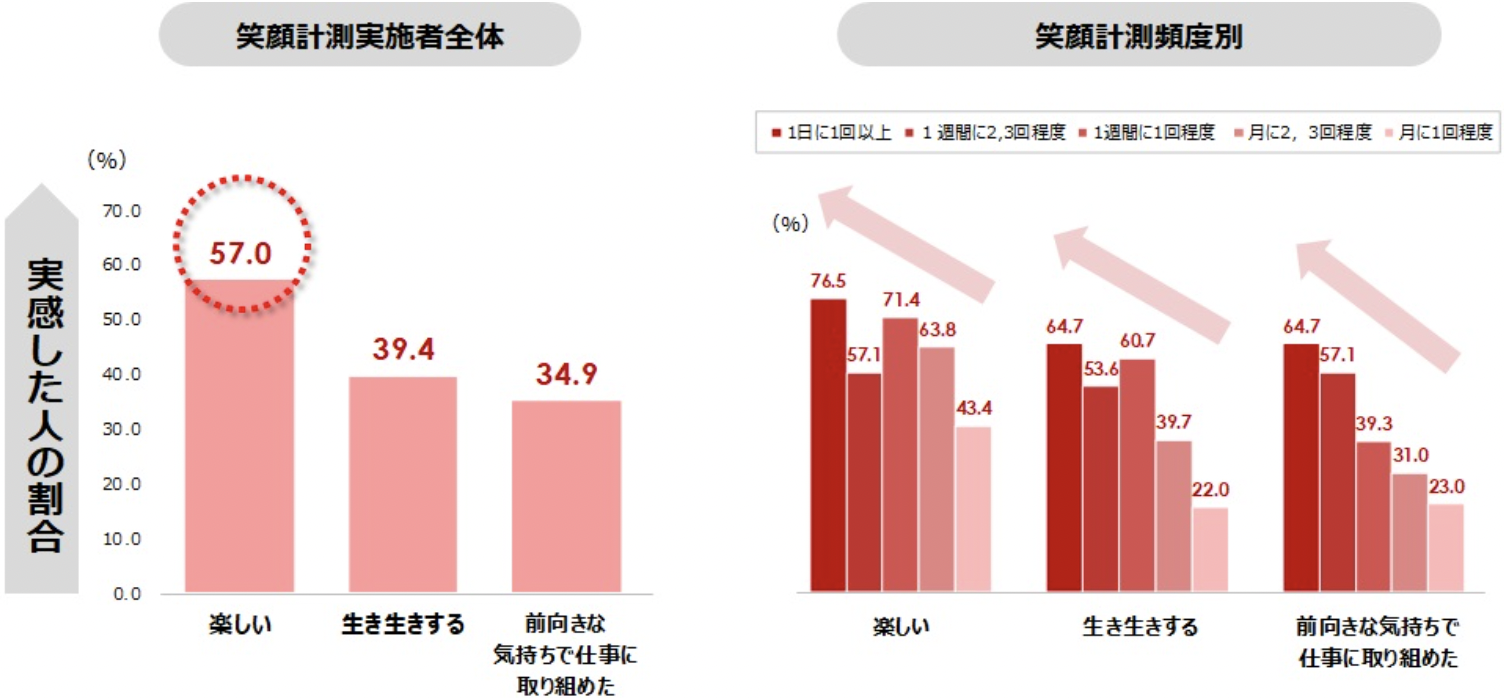
\includegraphics[scale=0.5, clip]{./img/work.png}
        \caption{笑顔計測後の主な感情変化}
        \label{fig:図の名前}
    \end{center}
\end{figure}

また,厚生労働省の調査[2]によると,下のグラフから分かるように,
平成19年度から令和元年にかけて約15\%も増加している.

\clearpage

\begin{figure}[!h]
    \begin{center}
        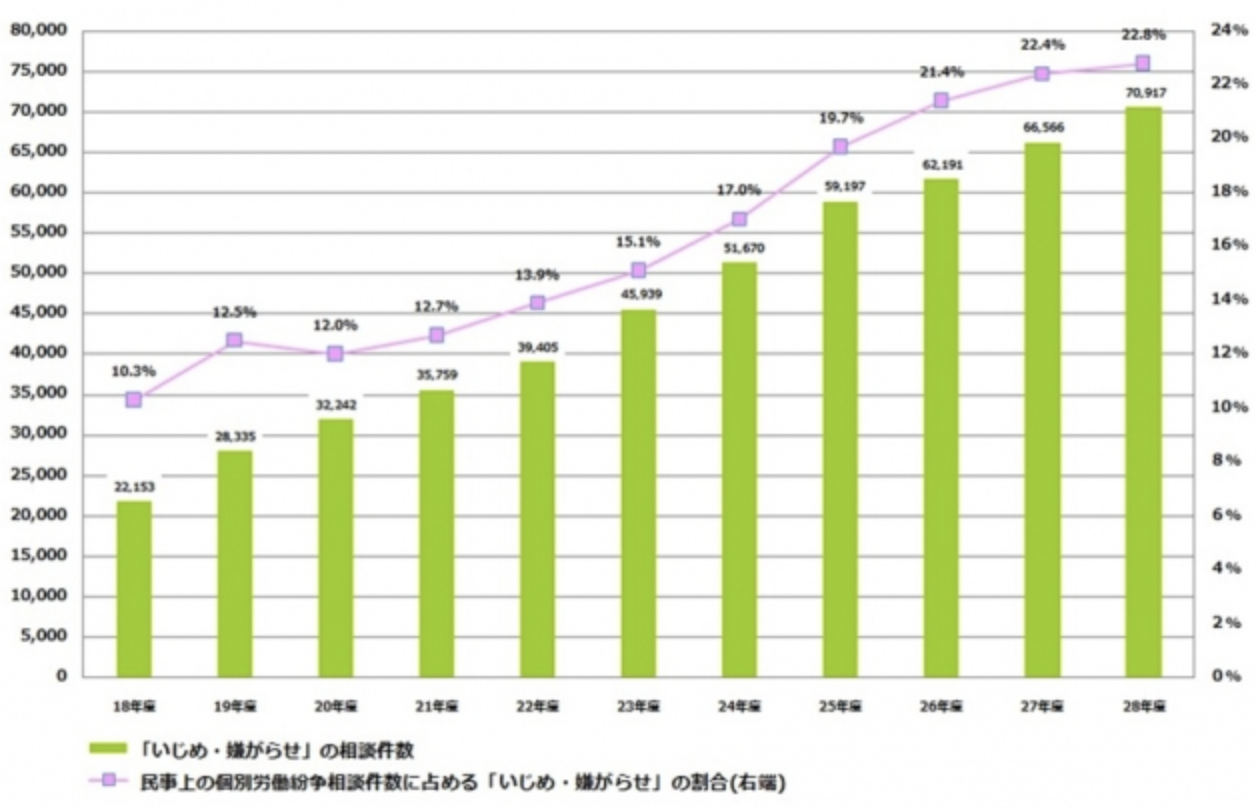
\includegraphics[scale=0.6, clip]{./img/graph.png}
        \caption{厚生労働省によるパワハラ調査}
        \label{fig:図の名前}
    \end{center}
\end{figure}

そこで我々は,以上の課題である「笑顔の減少」と「パワハラの増加」の解決を目的に
FaceAPIを用いた表情分析を活用した労務管理支援システムを提案する.

\section{論文の構成}
\label{sec:tex_basic_newline}
本論文は以下のような構成になっている.
\\
第 1 章では研究背景を述べる.
\\
第 2 章では本研究で開発する労務管理支援システムの概要を述べる.
\\
第 3 章では本研究で開発する労務管理支援システムの構成を述べる.
\\
第 4 章では本研究で開発する労務管理支援システムの実装結果を述べる.
\\
第 5 章では本研究のまとめを述べる.

\chapter{機能設計}
\label{chp:chart}

\section{FaceAPIを用いた労務管理支援システム}
\label{sec:chart_figure}
今回作成するシステムは,会社で使うことを想定しており,労務管理者と社員で使える機能を分ける.
次の章からそれぞれの機能について述べる.

\section{管理者用の機能}
\label{sec:chart_admin}
\subsection{社員管理}
社員管理は社員の名前,メールアドレス,社員番号などを表で管理する.さらにその表から名前などを編集
できる機能を実装する.

\subsection{掲示板}
労務管理者が社員に何かお知らせする際に利用できる.管理者しか発言できないようになっている.



\chapter{システムの実装方法}
\label{chp:reference}

\section{システム構成}
\label{sec:reference_ftnote}
本システムは以下のような構成で実装を行う.システム構成図を図3.1に示す.\\
労務管理支援システムをReactでWebアプリとして作成した.さらにデータベースにCloud Firestore,
ユーザー認証にFirebase Authentication,表情分析にface-api.jsを使用した。\\
 次のセクションでは,それぞれのサービスについて説明する.

\begin{figure}[!h]
	\begin{center}
			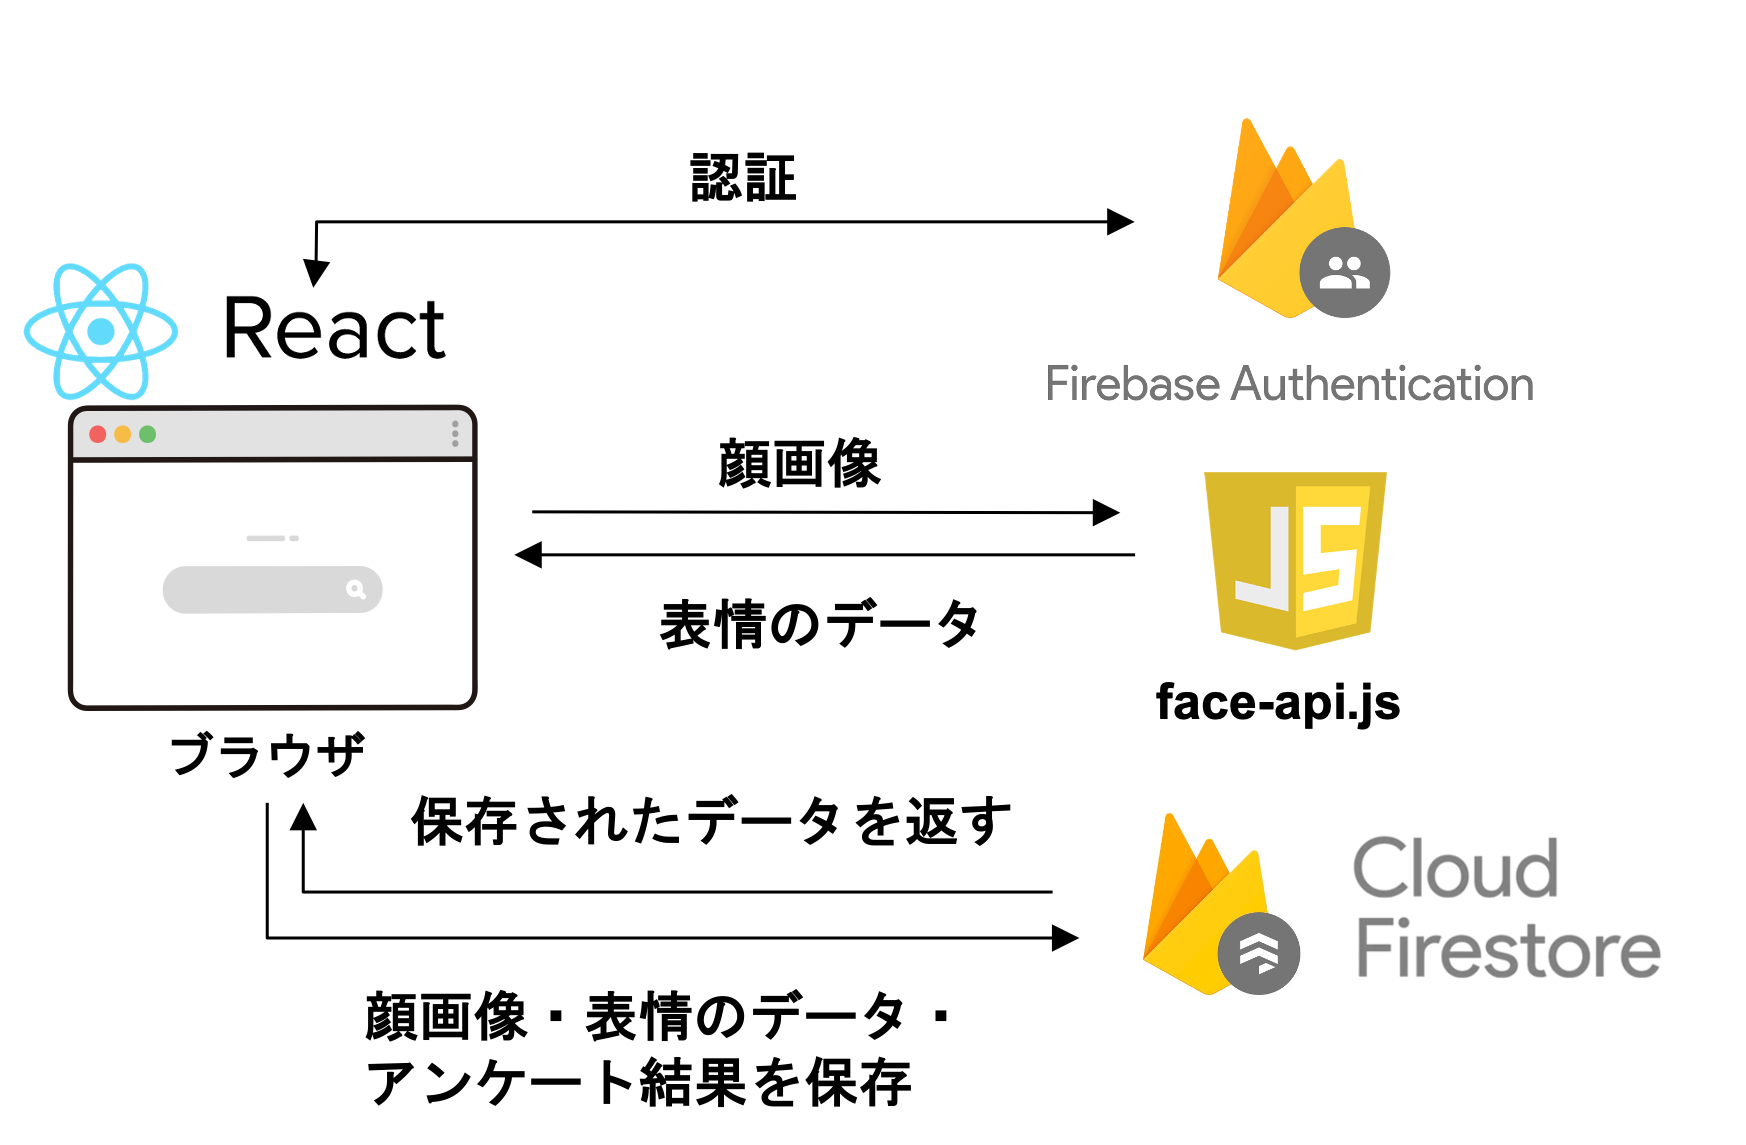
\includegraphics[scale=1.2, clip]{./img/compose.png}
			\caption{システム構成図}
			\label{fig:図の名前}
	\end{center}
\end{figure}


\section{React}
\label{sec:reference_quote}
Reactは,UI(ユーザインタフェース)部分の構築に特化したJavaScriptのライブラリで,
React.jsとも呼ばれる.
SNSで有名なMeta社(旧Facebook社)が自社サービスの機能拡張に伴うコードの複雑化によって
維持管理がしにくくなることを防ぐために開発した.
コーディングコストが少なく,開発規模が大きくなっても管理しやすいといった特長もあり,
現在では開発元であるFacebook社のサービスであるFacebookやInstagramはもちろんのこと,
Yahoo!やAirbnb,Reddit,Netflix,Slack,Uberといった世界的なWebサイトや
Webアプリで利用されるなど,世界中の多くの企業で採用されており,日本でも注目を集める
など,今最も勢いのあるライブラリである.
今回のシステム開発にReactを採用した理由は三つある.

	\begin{enumerate}
		\item パフォーマンスが良い \\
		Reactには,仮想DOM(Virtual Document Object Model)というレンダリング機構が
		備わっている.仮装DOMとは、実際のDOMではなく, React内部に持っている 
		DOMの情報である. Reactを使うと,この仮想DOMと実際のHTML上のDOMを
		比較したときに出てくる違いだけが,毎回HTML上に再適用される.
		そのため画面全体がReactで構成されていたとしても,必要な部分しか更新されず
		非常に高速に動作するため,パフォーマンスが良い.\\

		\item UIコンポーネントのライブラリが多い \\
		Reactは,世界中で使われているため,Reactのライブラリを使ってUIをコンポート化
		するようになってきている.あらかじめButtonやFormなどのUIパーツを
		Reactコンポーネントとして扱えるようにして,セット化したものが多くある.
		これらを使えば,今風の洗練された画面を作ることができる.\\

		\item JavaScriptの知識があれば使える \\
		基本的にReactはJavaScriptで書かれているため,
		JavaScriptの知識があればアプリを開発することができる.
		たとえJavaScriptの開発経験がなくても基本構文を理解していれば開発に
		取り掛かれる.今回,我々はJavaScriptの学習を既に行なっていたので,
		Reactを選んだ.
	\end{enumerate}
	
\section{face-api.jsについて}
\label{sec:reference_bib}
face-api.jsはブラウザ, NodeJSで顔を検出するための,
Tensorflow.jsを活用したJavaScript APIである.
顔検出,顔のランドマーク検出,顔検出,表情認識,年齢推定,性別認識といった
モデルが利用できる.本研究では,社員の提出した写真から表情分析を行い,
怒り,驚き,恐怖,嬉しさ,うんざり,中立,悲しさといった7つの表情に分解することを目的とする.
そして,それらをグラフ化して表示する.
	
\section{Material-UIについて}
\label{sec:reference_chapter}



\chapter{動作検証}
\label{chp:tex_pro}
この章では動作検証の結果をスクリーンショットとソースコードを元に紹介する.
今回はGoogle Chrome上で動作させるため,他のWebブラウザ上ではUIが異なっている可能性がある.

\section{社員が写真を提出する}
\label{sec:tex_pro_cmd}
社員ページに顔写真提出するためのフォームを作成した.写真提出ボタンから提出する写真を選択し,
提出する.その実行しているスクリーンショットを図4.1,図4.2,図4.3,図4.4に示す.

もし顔認識できない写真であれば,もう一度写真を提出させる処理をすることでエラー回避している
(ソースコード4.1).そのスクリーンショットを図4.5に示す.

\begin{lstlisting}[caption=顔認識エラー処理]
  if (object.length !== undefined) {
    return (
      <div>
        <p>顔認識できません。</p>
        <p
          className="submit reset"
          onClick={() => {
            setNum(1);
          }}
        >
          やり直す
        </p>
      </div>
    );
  }
\end{lstlisting}

\vspace{4mm}

\begin{figure}[!h]
	\begin{center}
			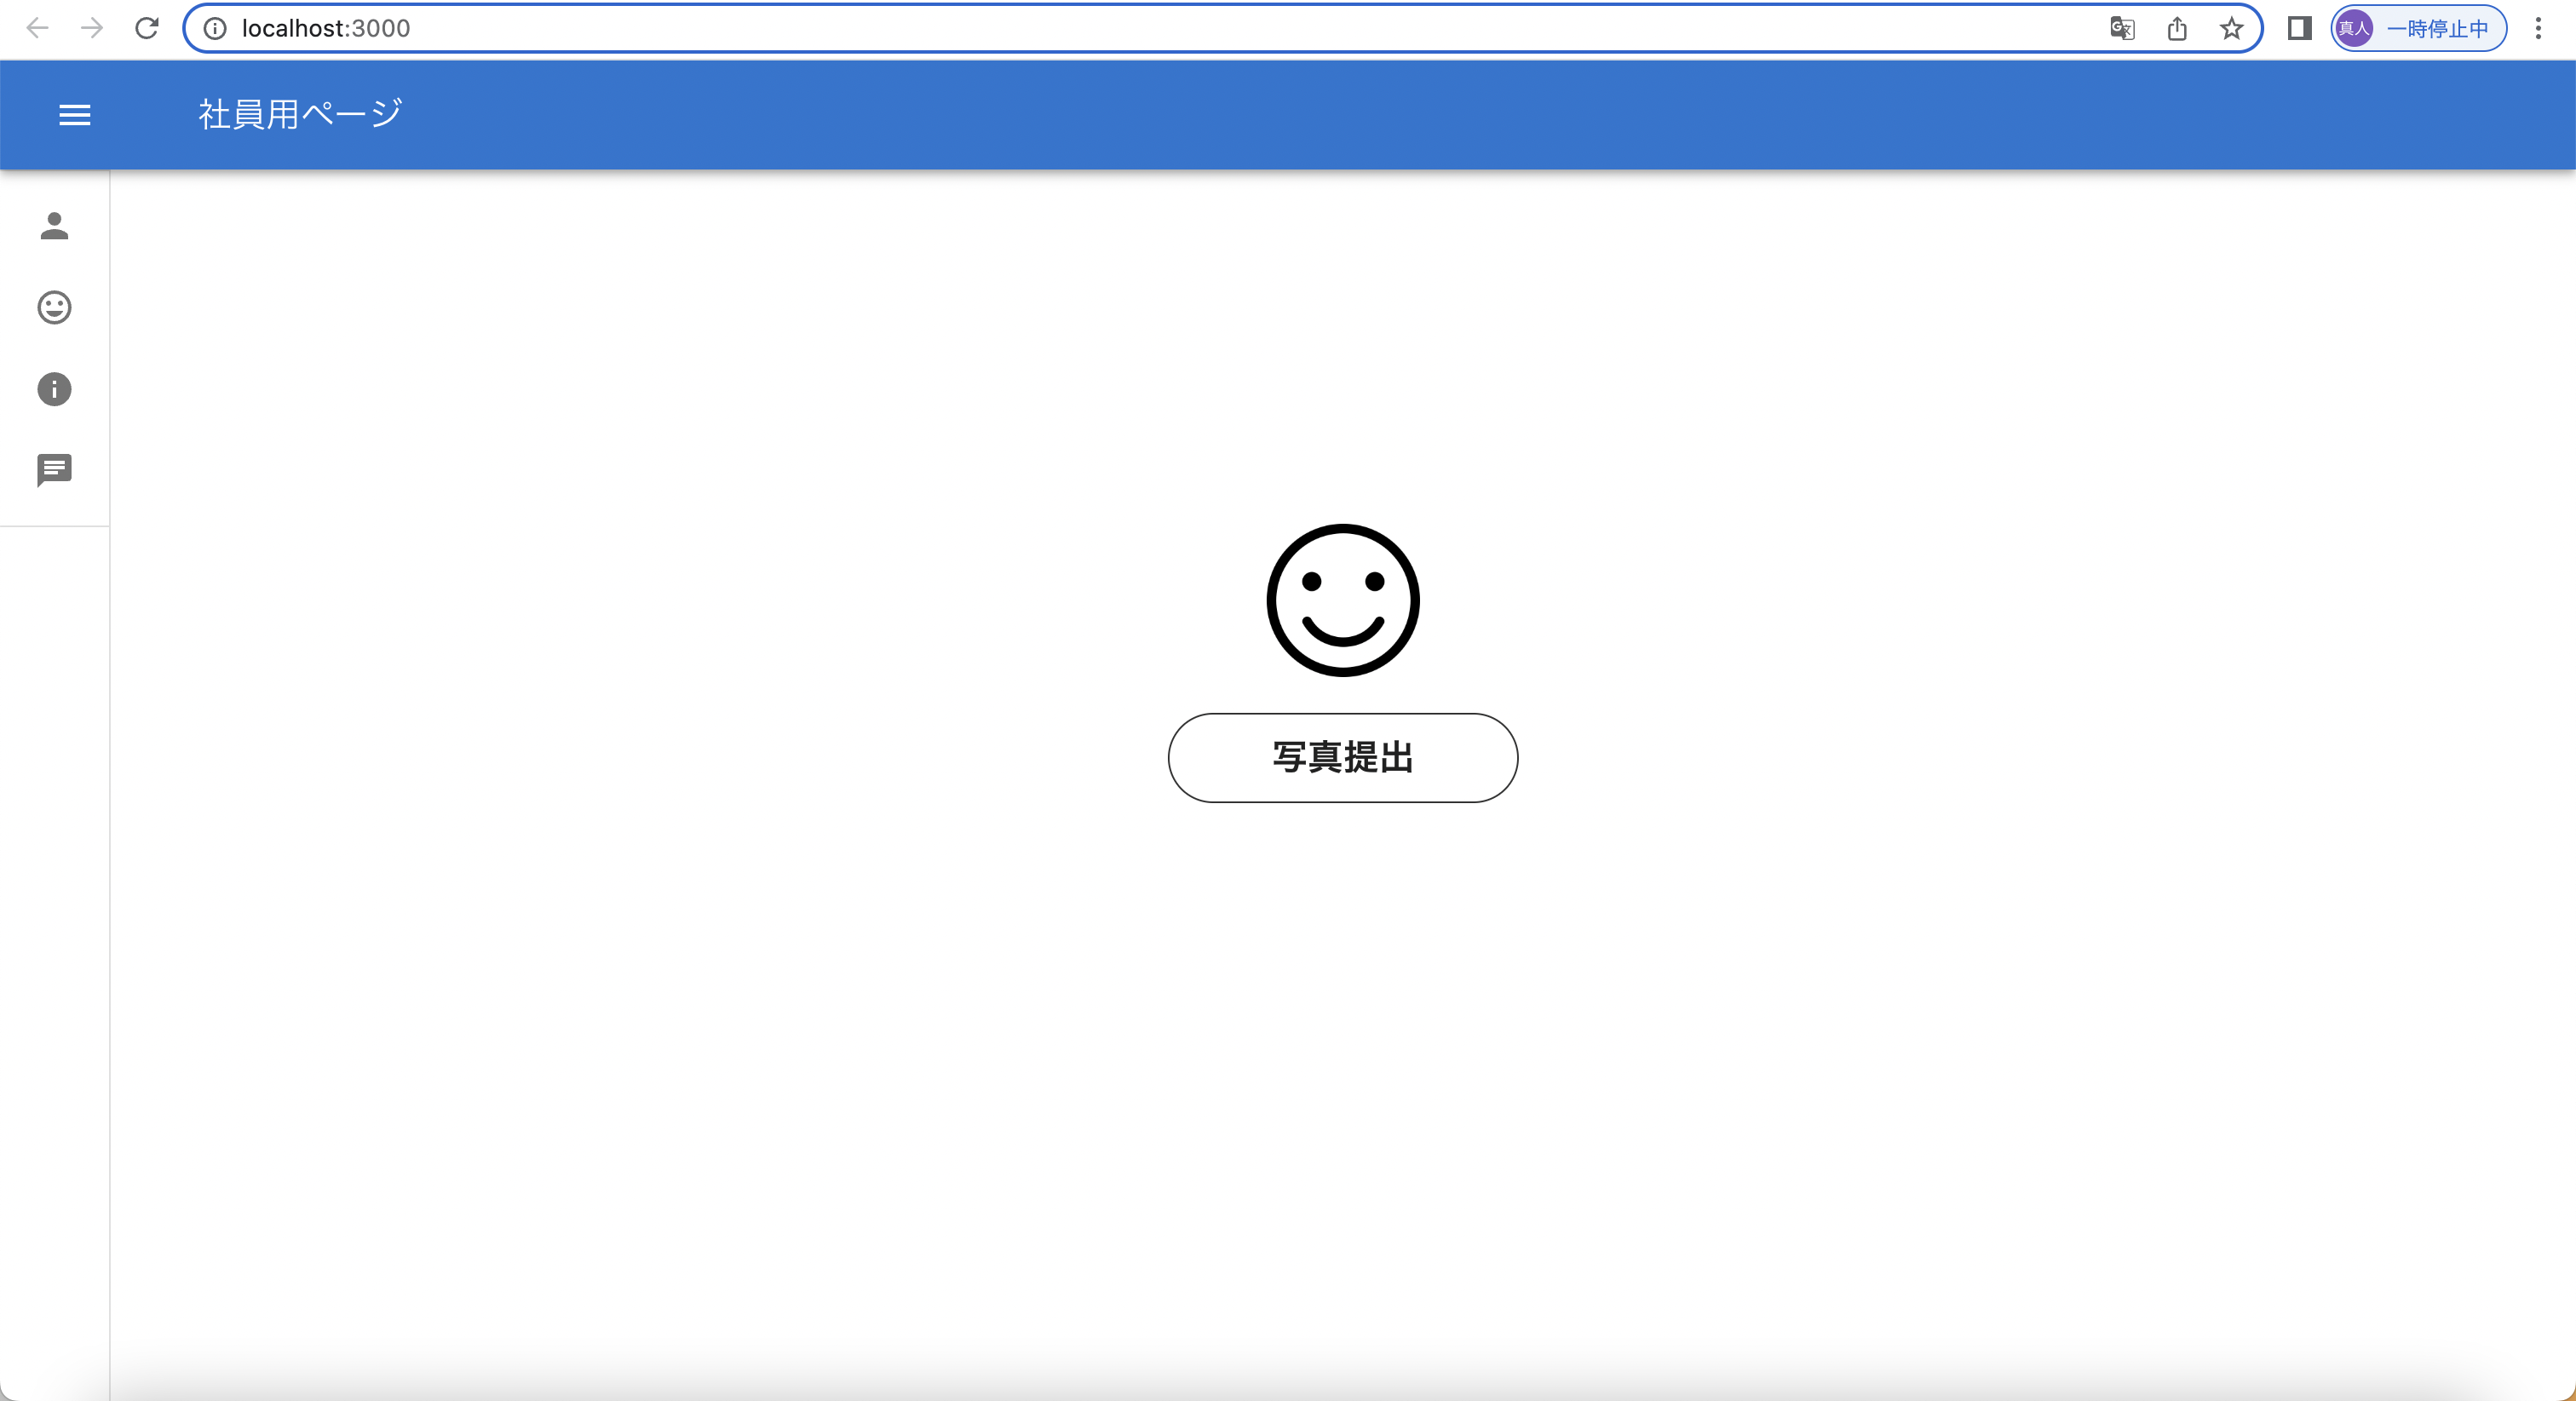
\includegraphics[scale=0.3, clip]{./img/sample1.png}
			\caption{提出画面}
			\label{fig:図の名前}
	\end{center}
\end{figure}

\begin{figure}[!h]
	\begin{center}
			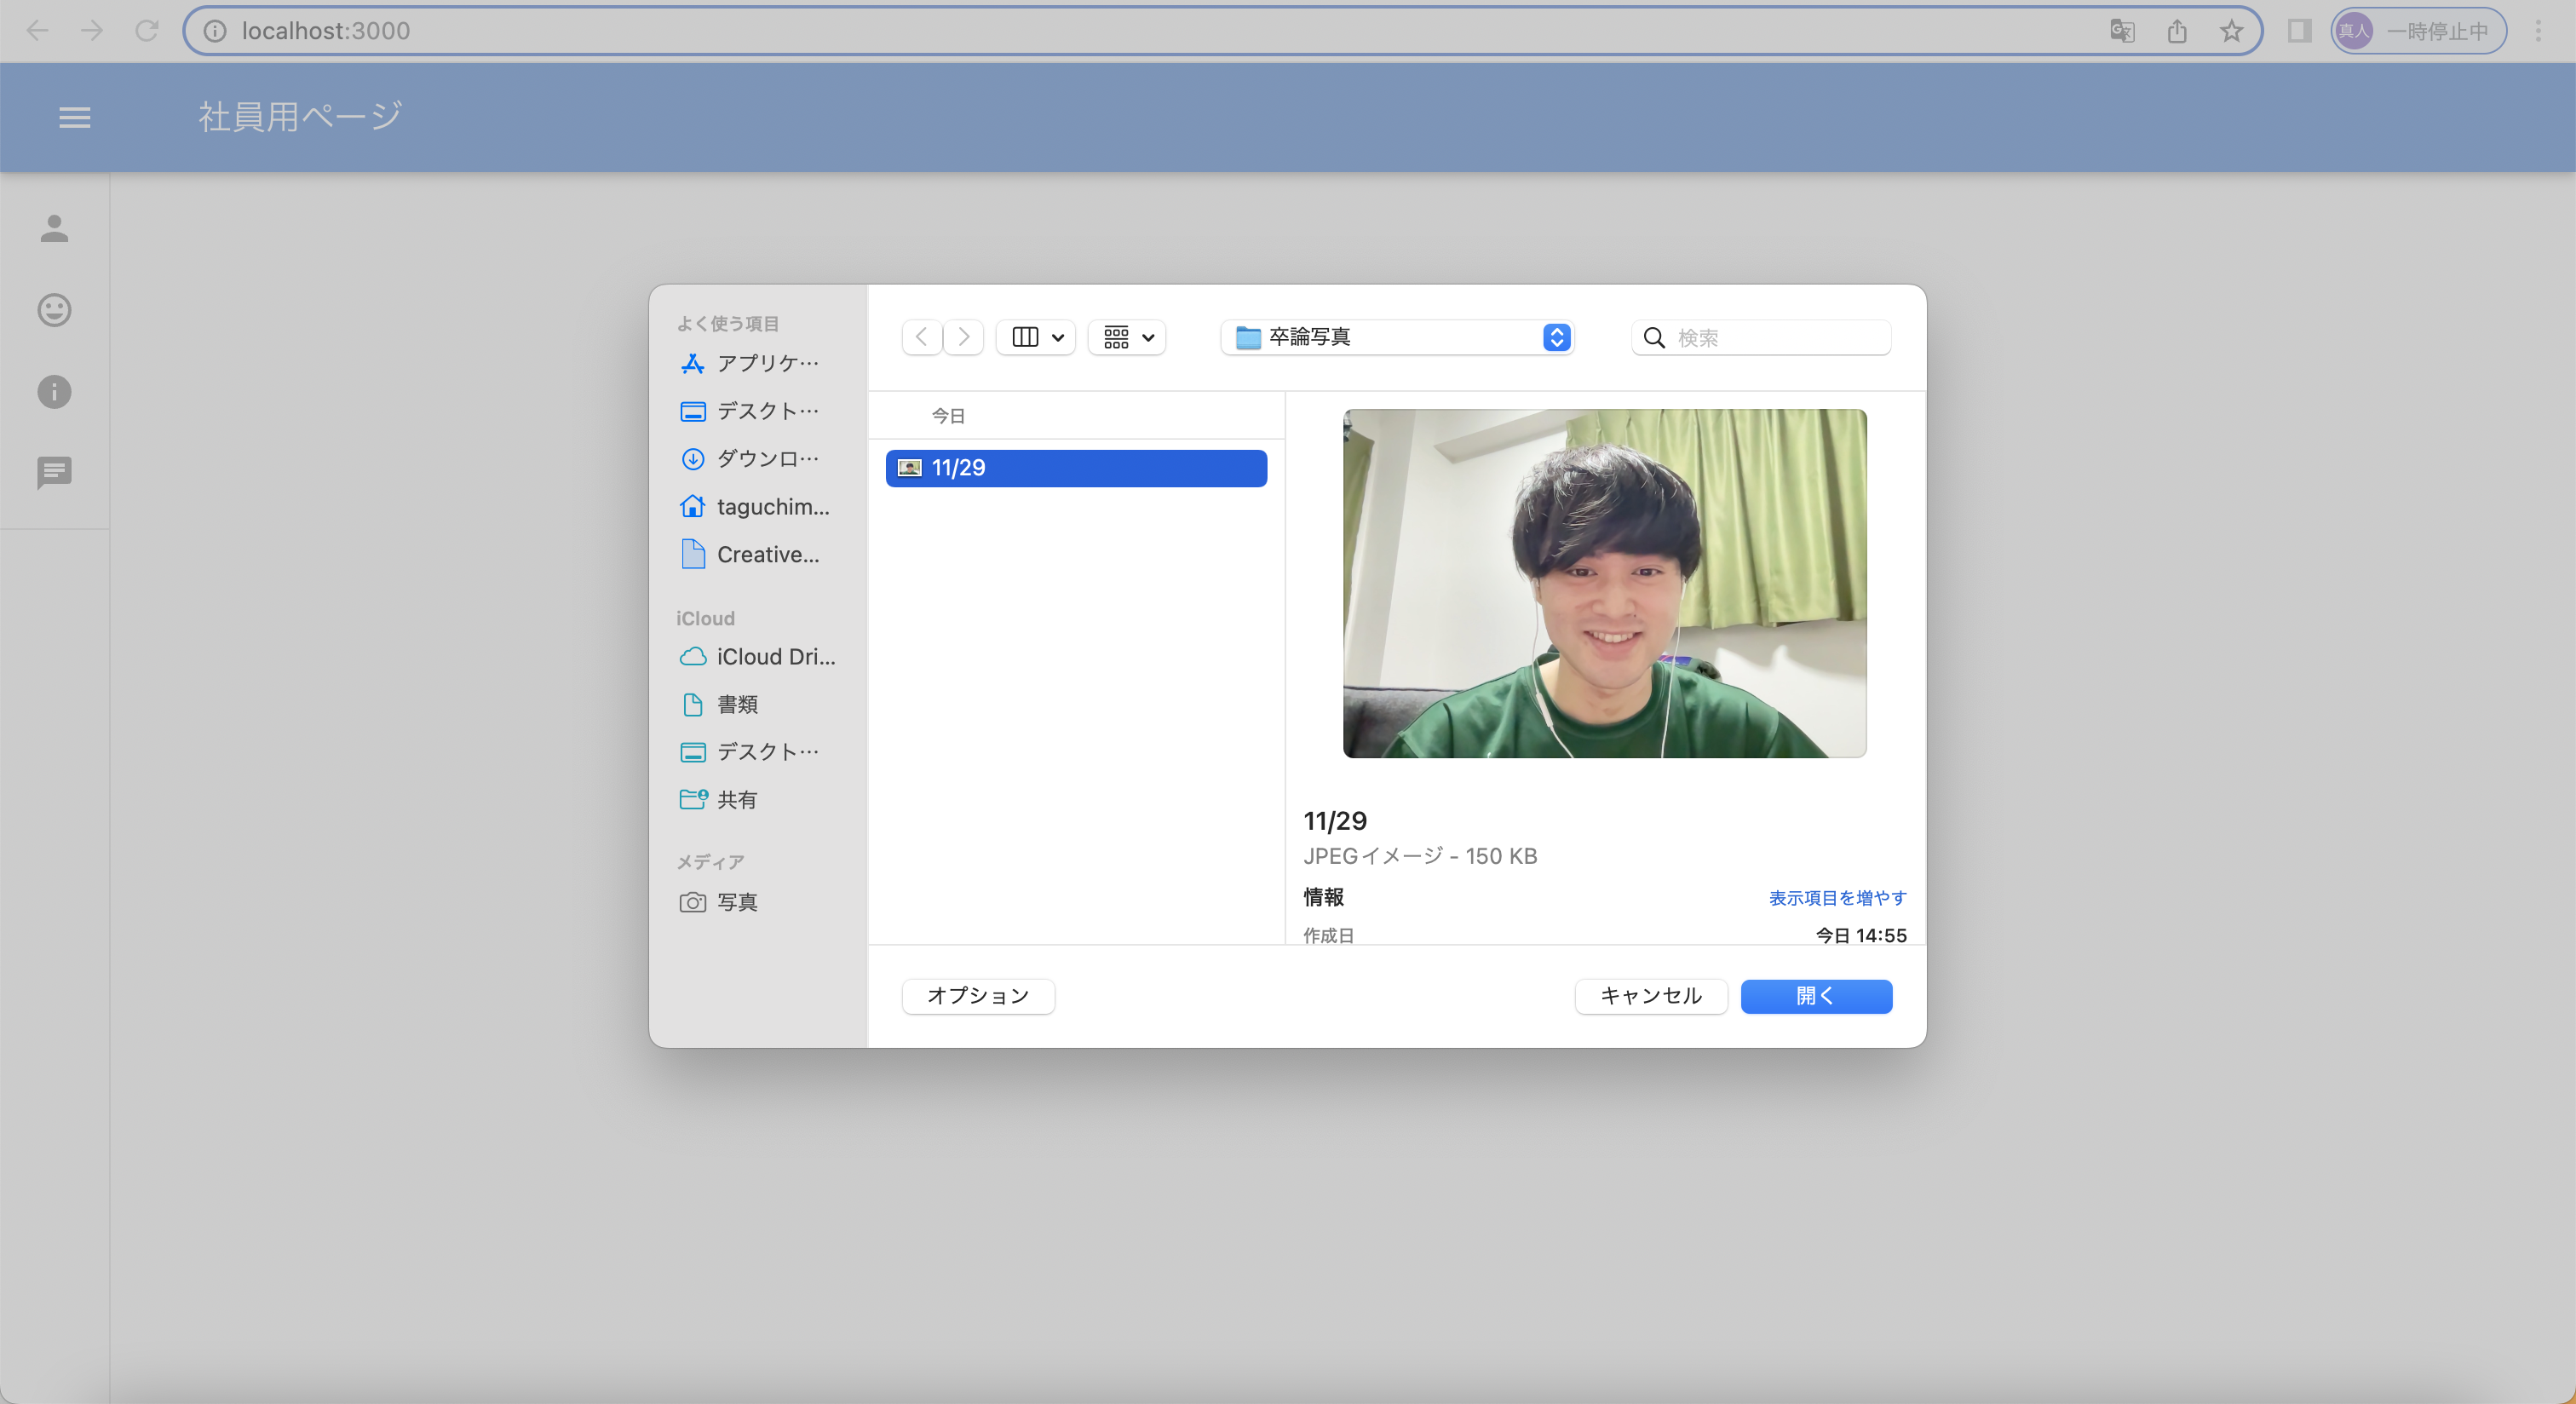
\includegraphics[scale=0.3, clip]{./img/sample2.png}
			\caption{写真選択画面}
			\label{fig:図の名前}
	\end{center}
\end{figure}

\begin{figure}[!h]
	\begin{center}
			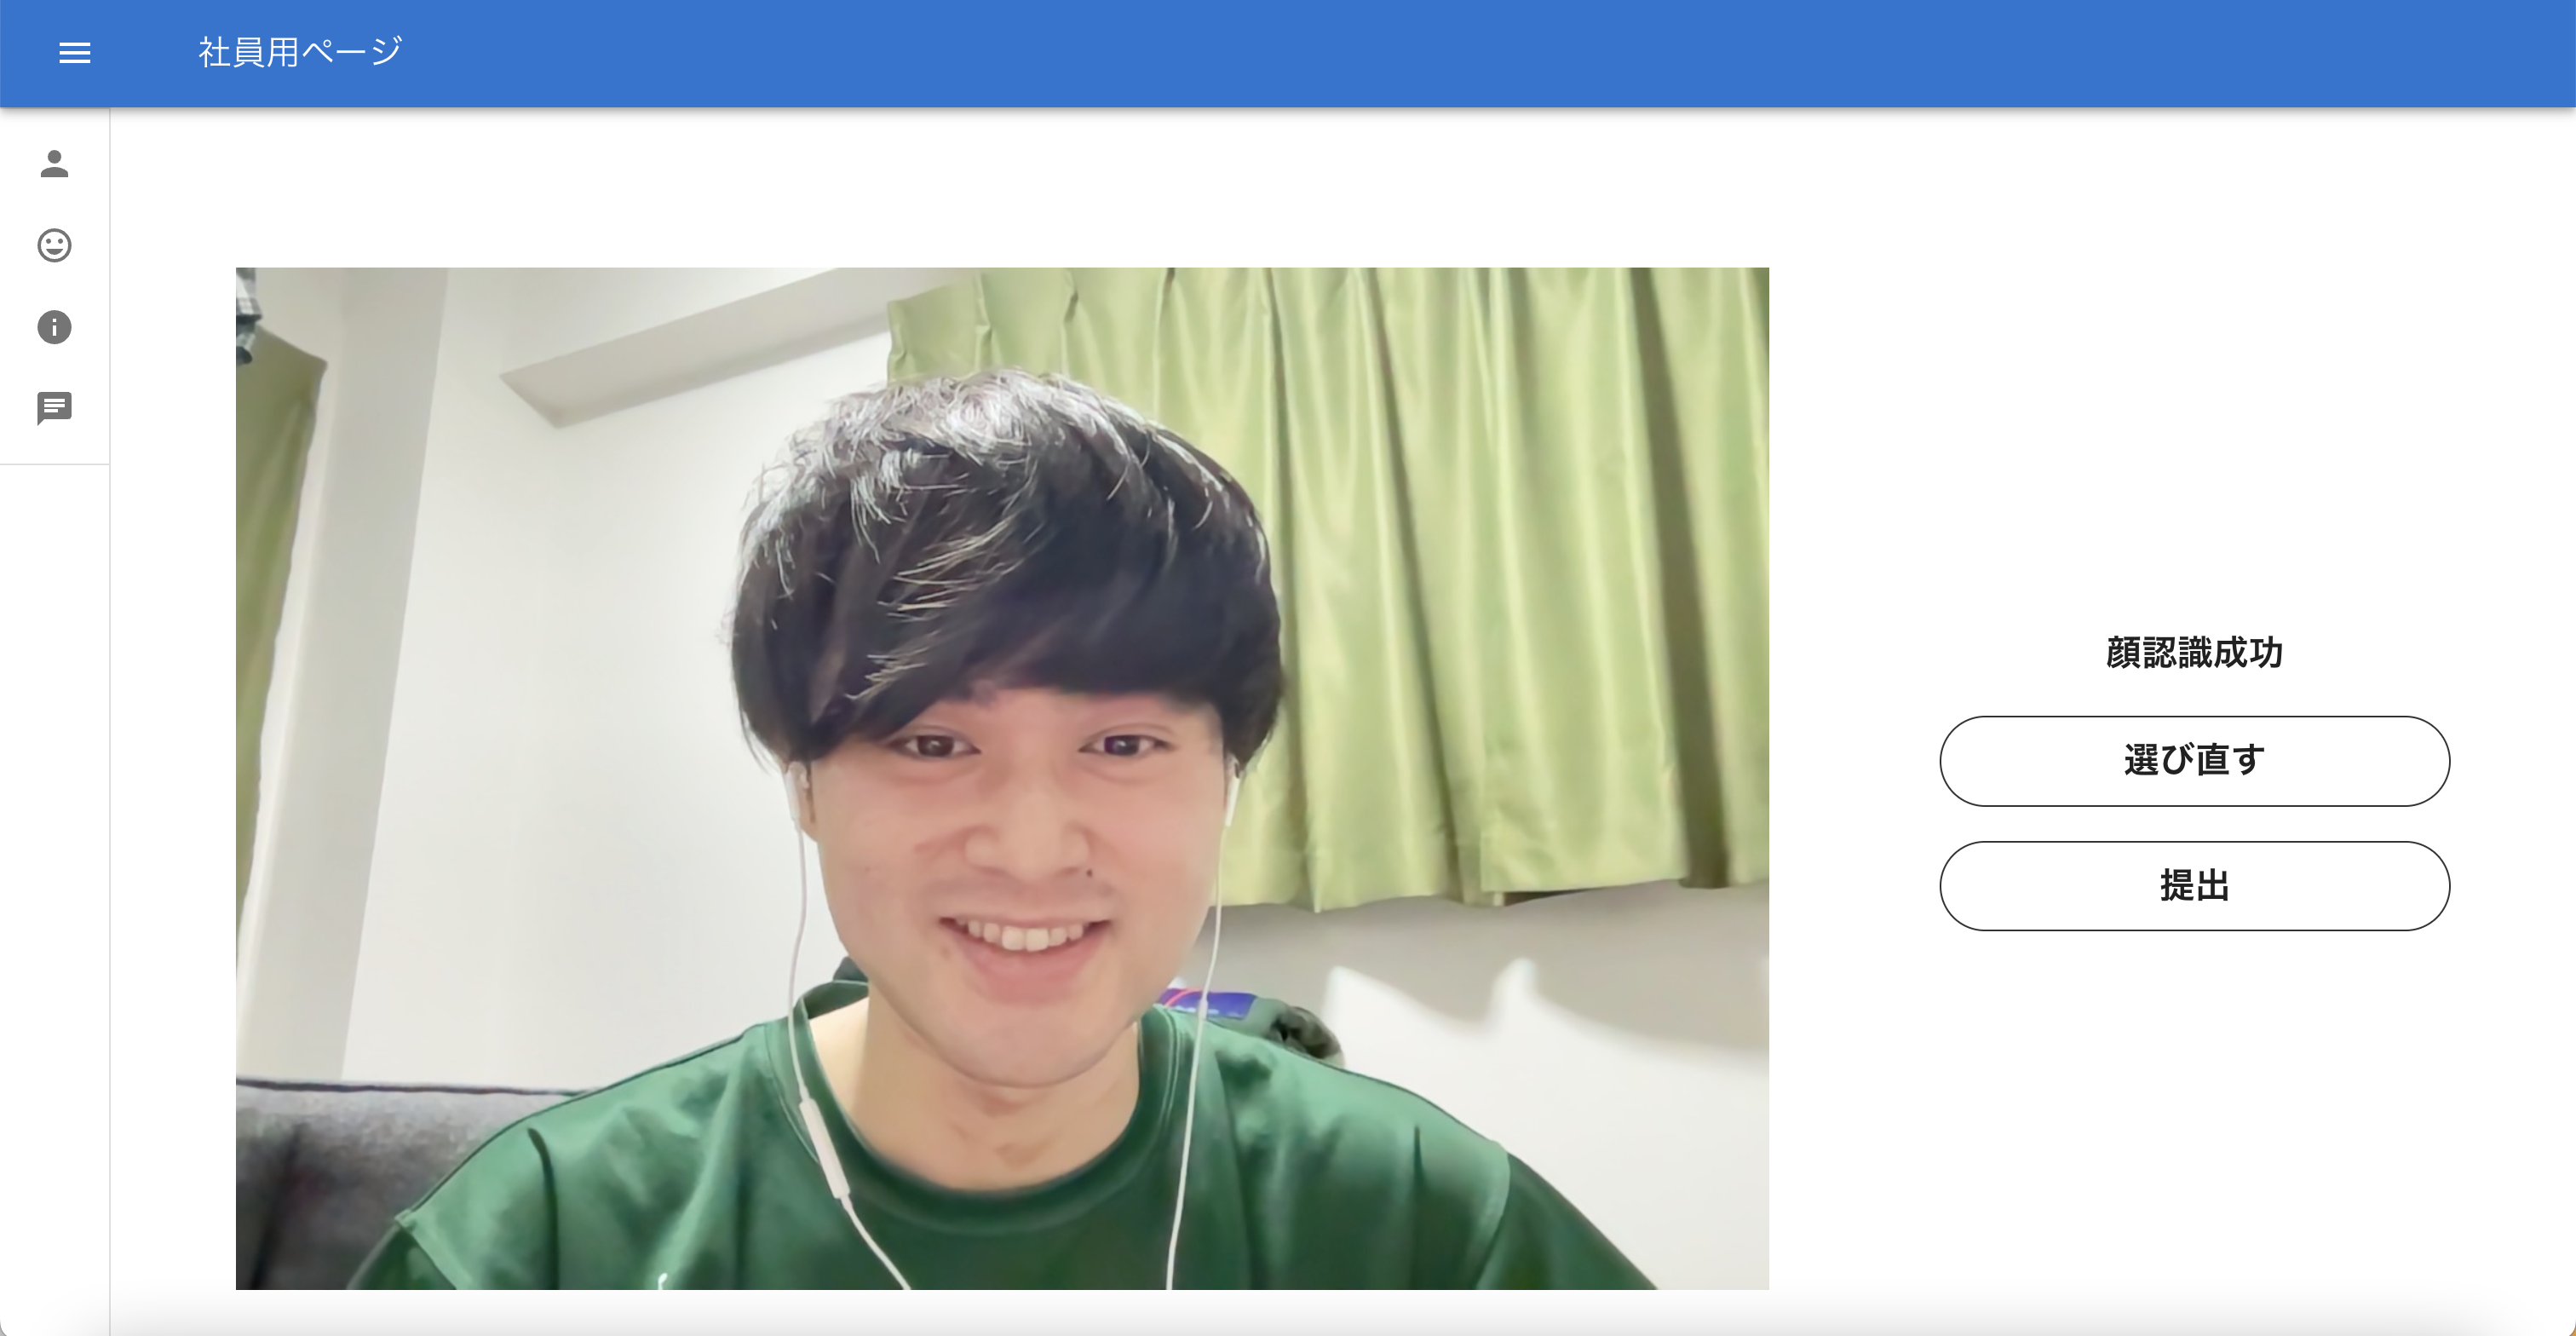
\includegraphics[scale=0.3, clip]{./img/sample3.png}
			\caption{画面}
			\label{fig:図の名前}
	\end{center}
\end{figure}

\begin{figure}[!h]
	\begin{center}
			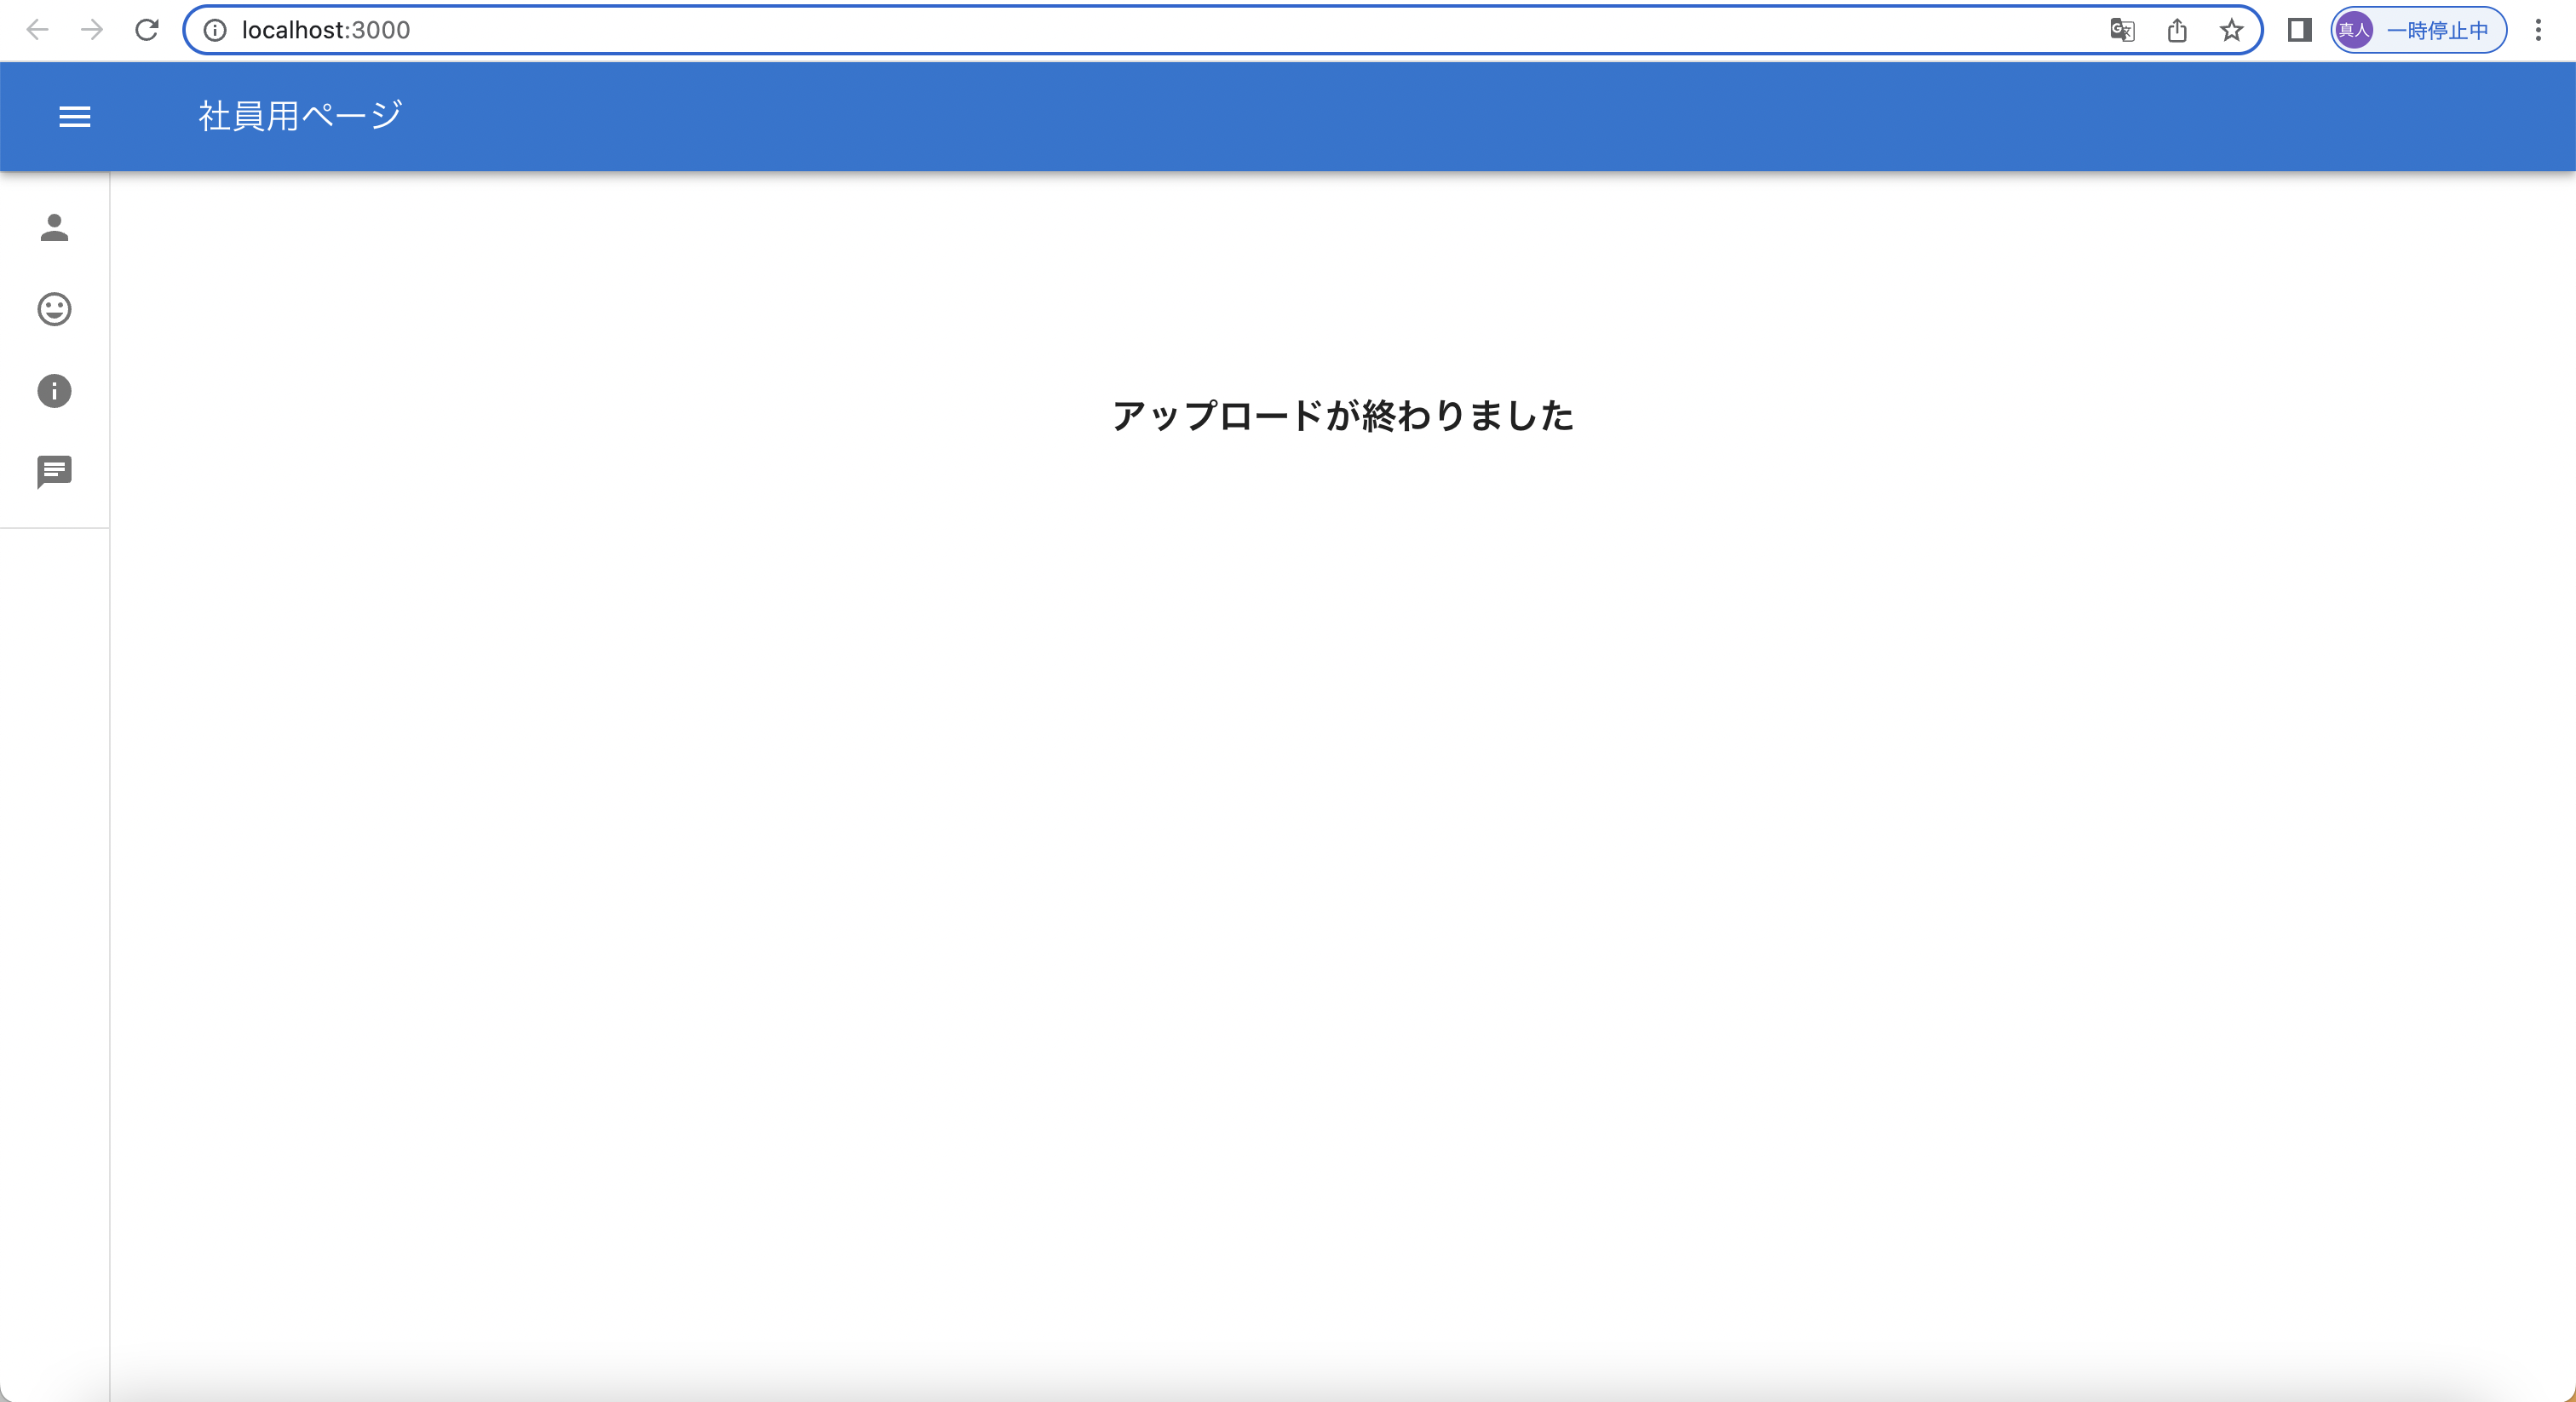
\includegraphics[scale=0.3, clip]{./img/sample4.png}
			\caption{提出完了画面}
			\label{fig:図の名前}
	\end{center}
\end{figure}

\clearpage

\begin{figure}[!h]
	\begin{center}
			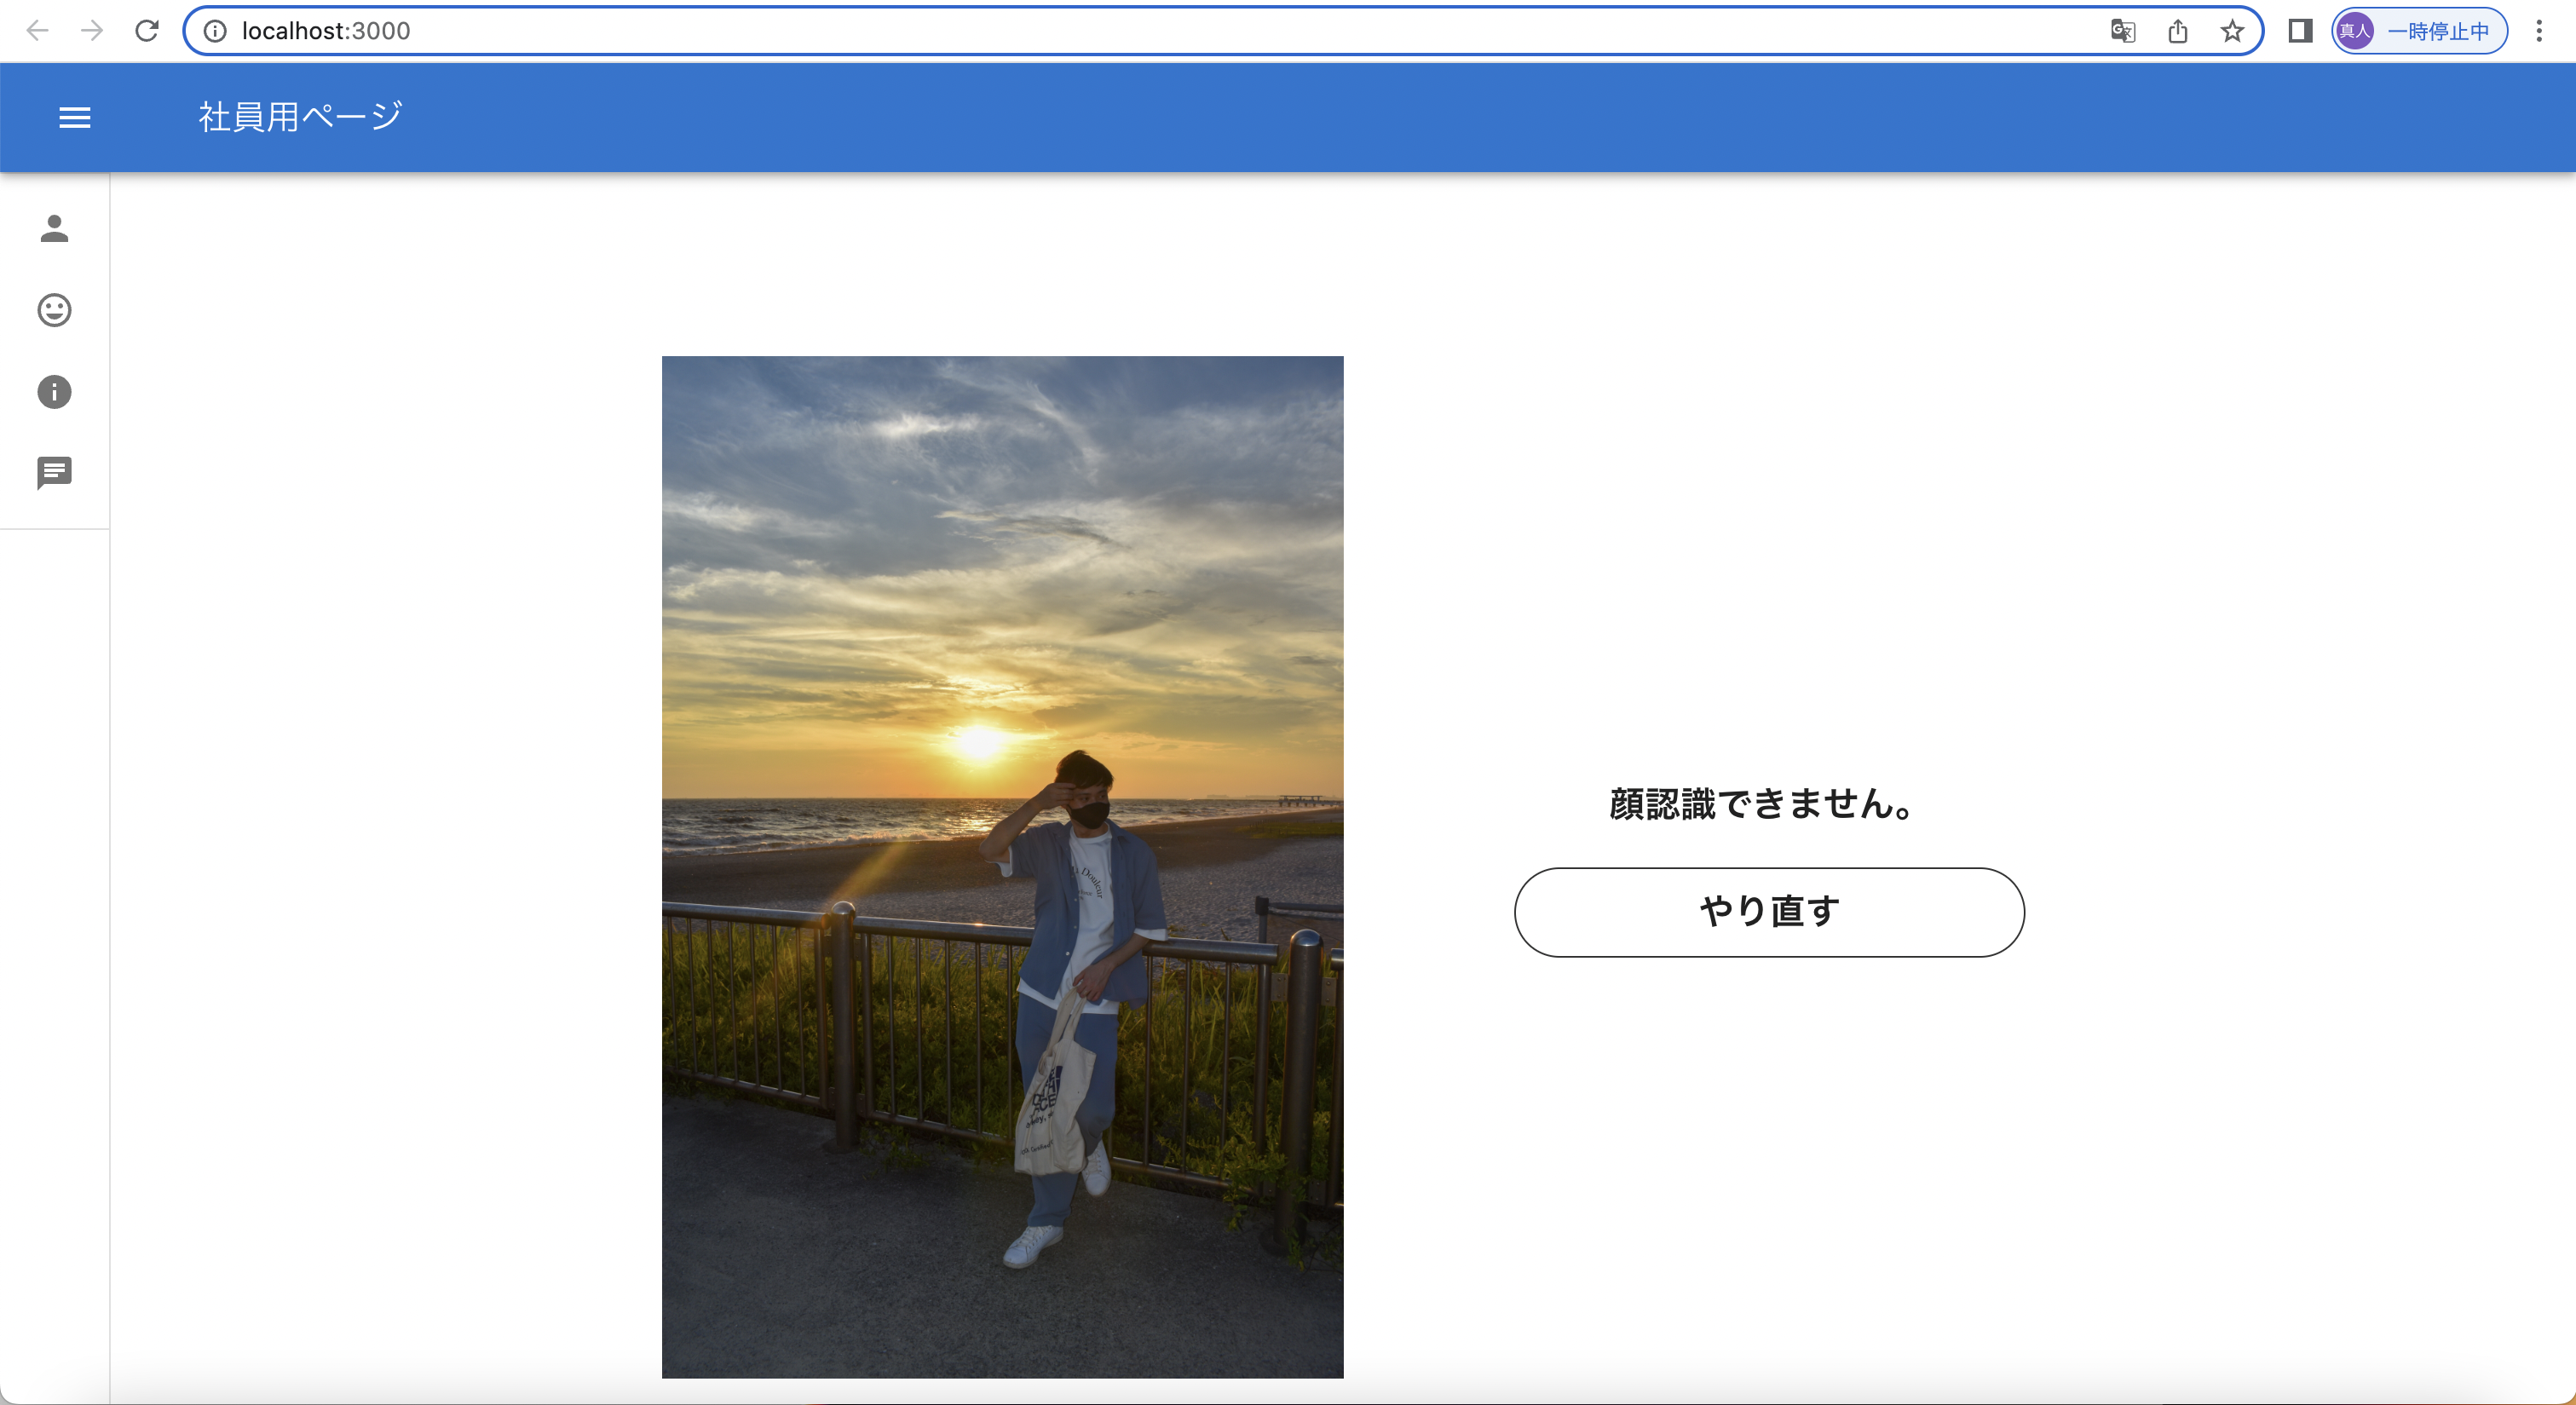
\includegraphics[scale=0.3, clip]{./img/sample5.png}
			\caption{顔認識失敗画面}
			\label{fig:図の名前}
	\end{center}
\end{figure}

\section{管理者の社員管理機能}
\label{chp:tex_admin}
管理者ページでは,管理者が社員を管理しやすくするために,表で管理しており,
社員ID,名前,メールアドレス,笑みポイントを可視化している.
図4.6に表が表示されているスクリーンショットを示す.
その他に,それぞれの社員の名前やメールアドレスなどを編集できる機能,提出された写真を見る機能,
社員とトークできる機能がある.それぞれについて,以下で説明する.

\subsection{編集機能}
編集ページのスクリーンショットを図4.7に示す.
編集機能では,社員ID,笑みポイント,役職,名前,メールアドレスを編集できる.
編集した社員IDが他の社員IDと被ってしまうとエラーが起きてしまうので,ソースコード4.2,
ソースコード4.3の様にしてエラー回避している.変数querySnapshot2でidが被っているユーザーを
検索し,変数qに配列として代入している.idが一つでも被っていたらqの大きさは0では無くなるので,
ソースコード4.2の9行目から始まるif文とソースコード4.3でidが被った際の処理をしている.
その際のスクリーンショットを図4.8に示す.

\clearpage

\begin{lstlisting}[caption=社員IDが被った時の処理]
  const handleSubmit = async (event) => {
    event.preventDefault();
    const data = new FormData(event.currentTarget);
    const id = Number(data.get("id"));
    const querySnapshot2 = await getDocs(
      query(collection(db, "users"), where("id", "==", id)));
    const q = querySnapshot2.docs.map((doc) => doc.id);

    if (q.length === 0) {
      setNum(2);
      // db更新
      const querySnapshot = await getDocs(
        query(collection(db, "users"), where("id", "==", props.count))
      );
      const docId = querySnapshot.docs.map((doc) => doc.id).toString();
      await updateDoc(doc(db, "users", docId), {
        id: Number(data.get("id")),
        name: data.get("name"),
        email: data.get("email"),
        point: Number(data.get("point")),
        role: data.get("role"),
      });
    } else {
      setNum(3);
    }
  };
\end{lstlisting}

\begin{lstlisting}[caption=社員IDが被った時の処理]
  else if (num === 3) {
    return (
      <div>
        <ArrowBackRoundedIcon
          sx={{ fontSize: 60 }}
          className="back"
          onClick={() => {setNum(0);}}
        />
        <p>idが被っています</p>
      </div>
    );
  }
\end{lstlisting}

\begin{figure}[!h]
	\begin{center}
			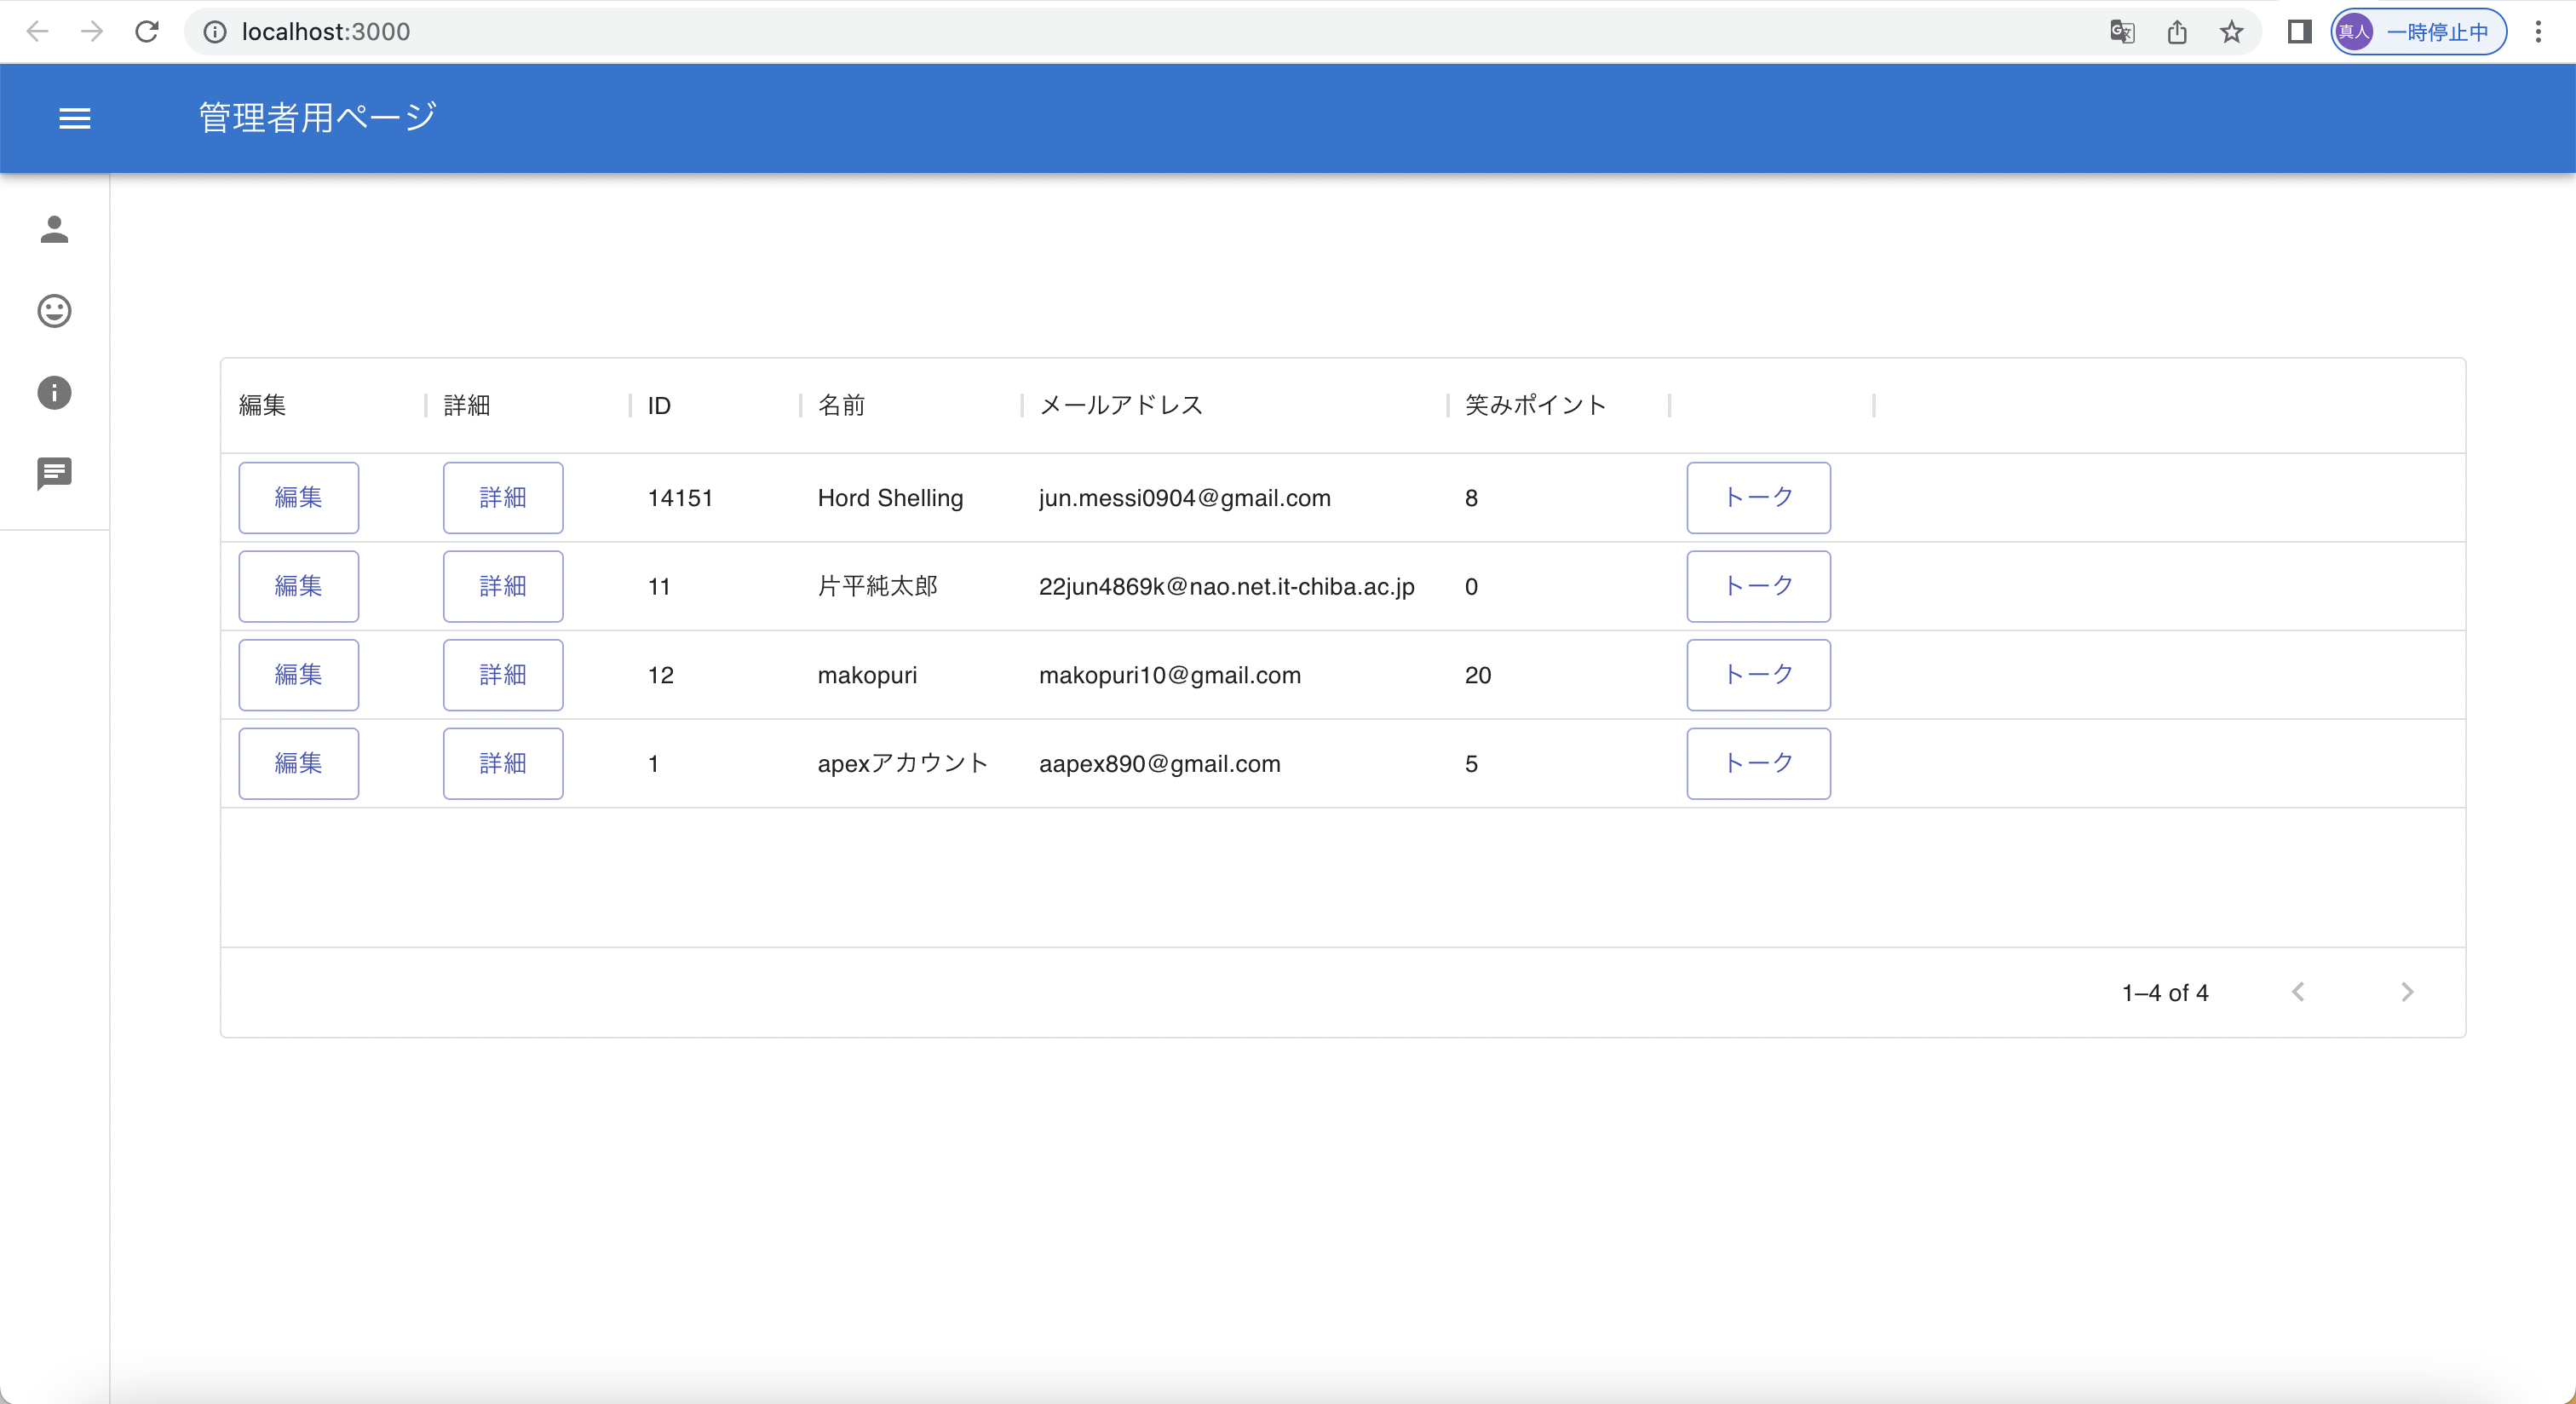
\includegraphics[scale=0.3, clip]{./img/sample6.png}
			\caption{社員管理画面}
			\label{fig:図の名前}
	\end{center}
\end{figure}

\begin{figure}[!h]
	\begin{center}
			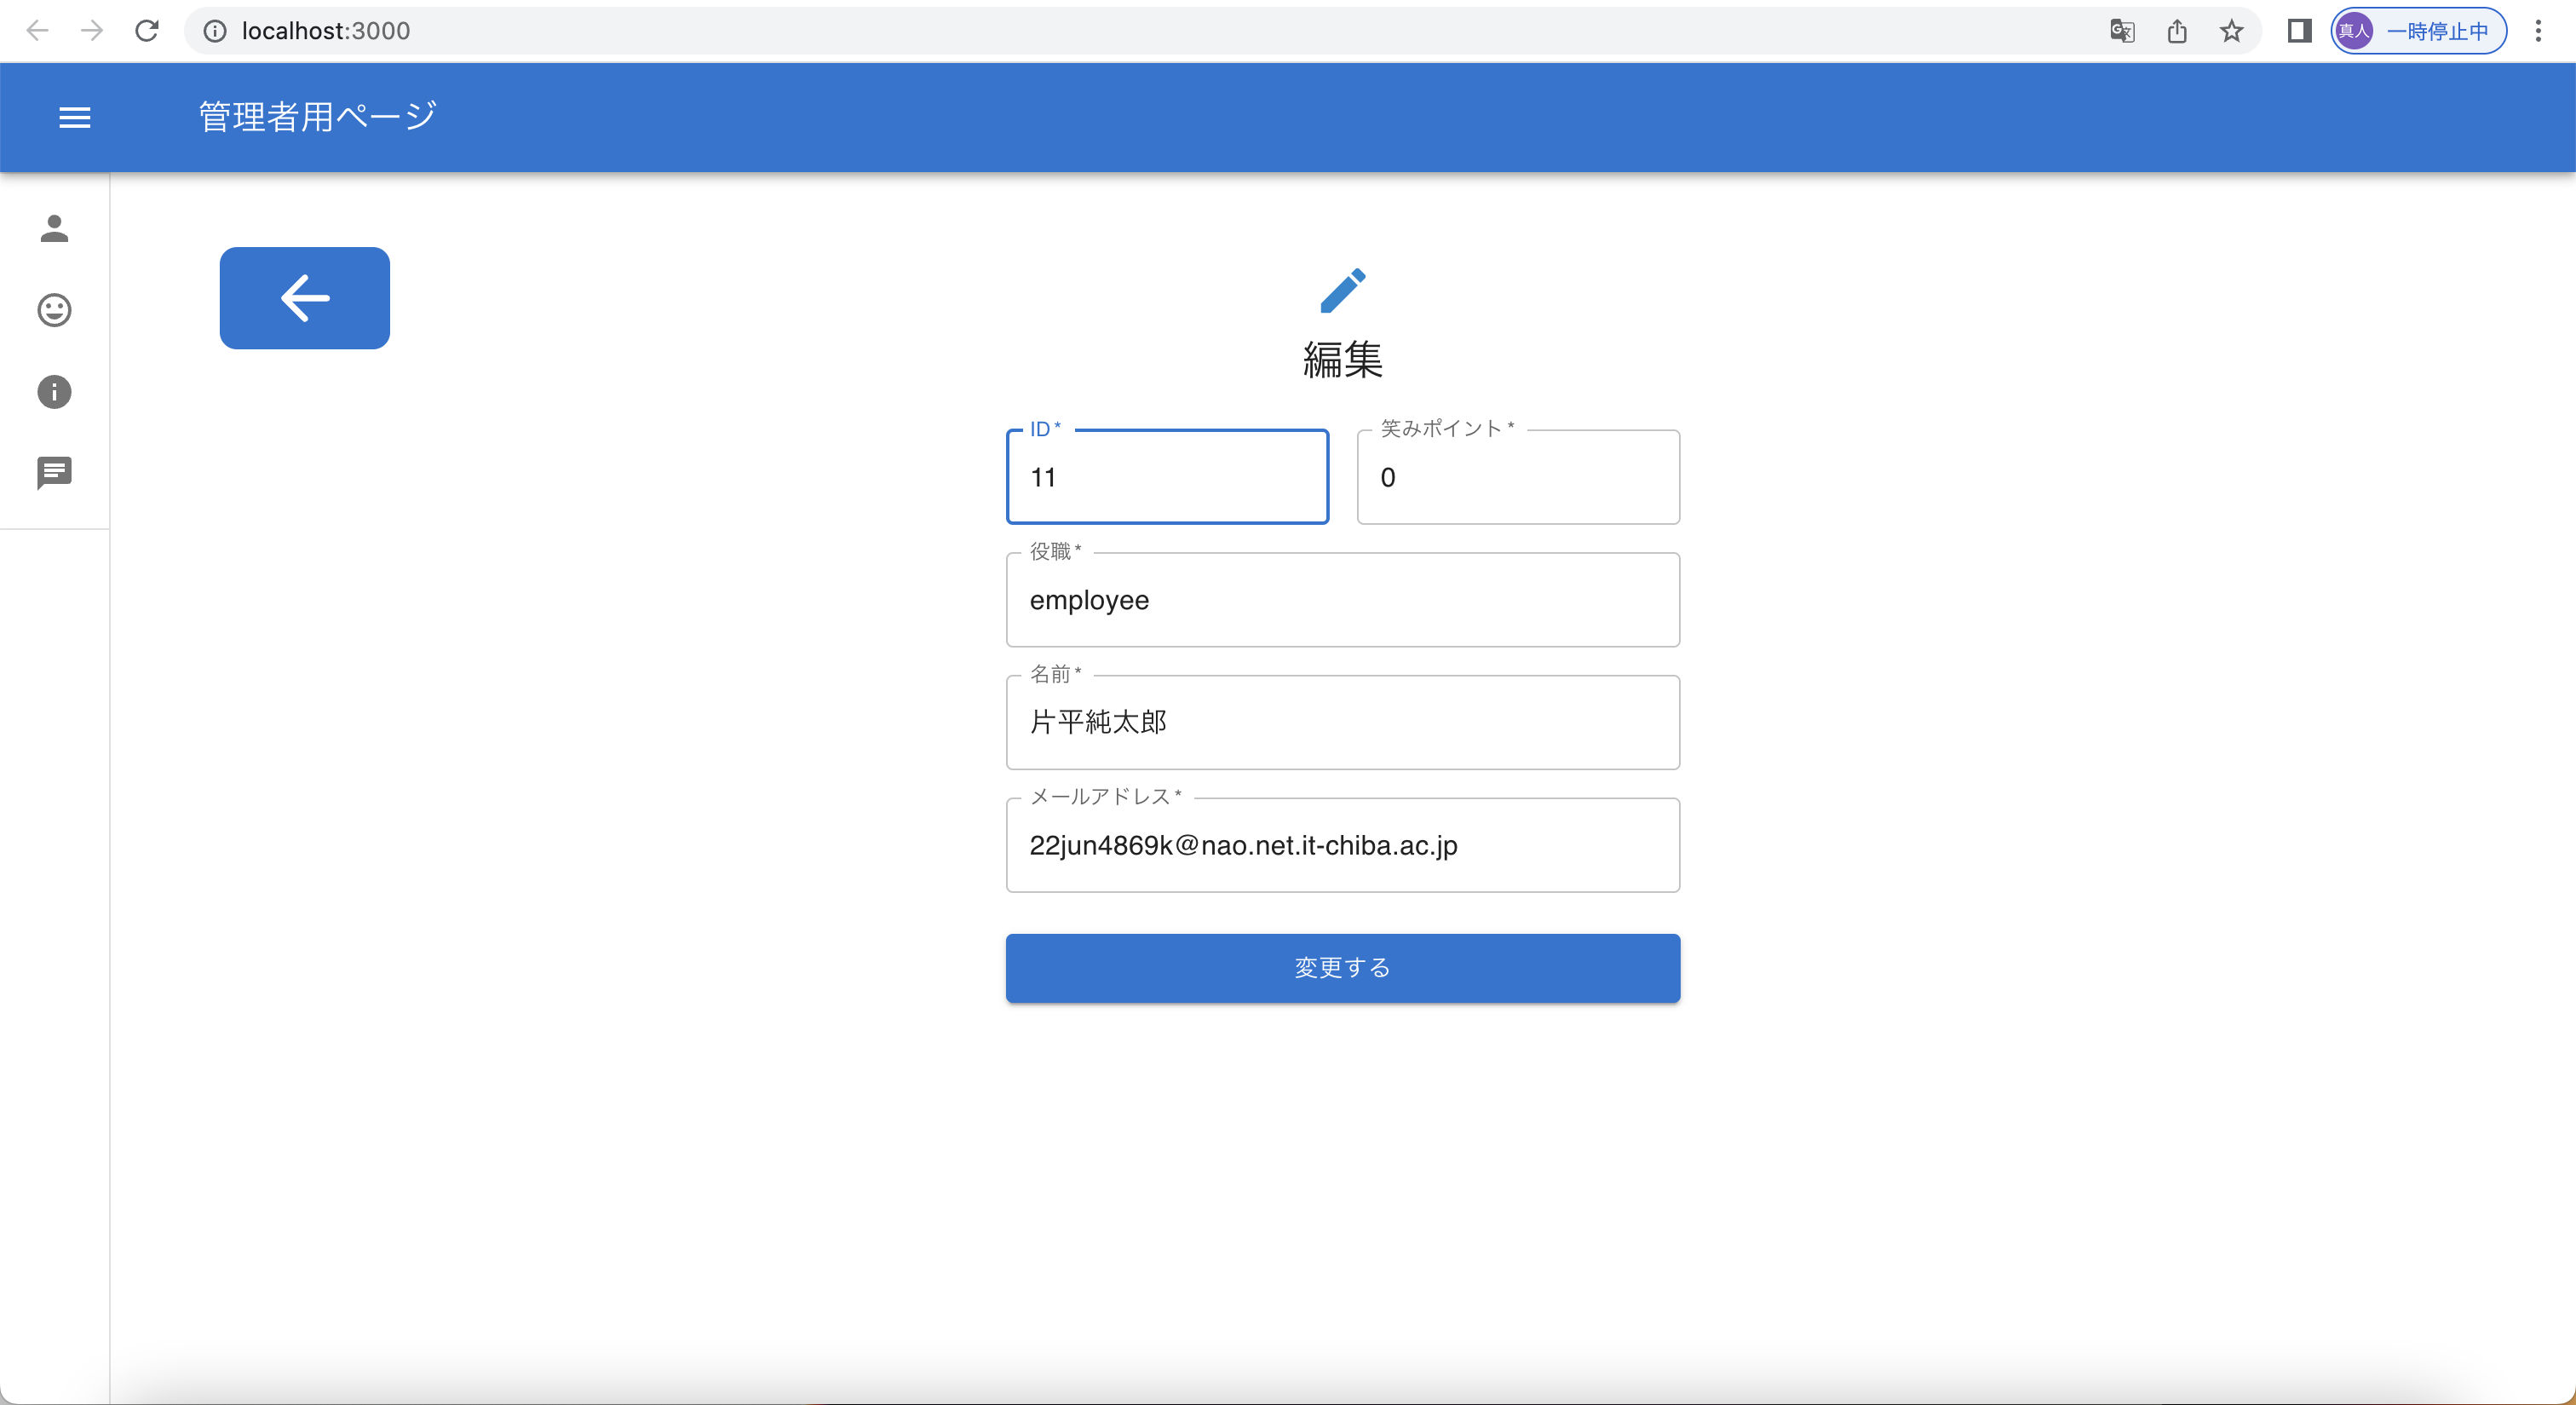
\includegraphics[scale=0.3, clip]{./img/sample7.png}
			\caption{編集画面}
			\label{fig:図の名前}
	\end{center}
\end{figure}

\clearpage

\begin{figure}[!h]
	\begin{center}
			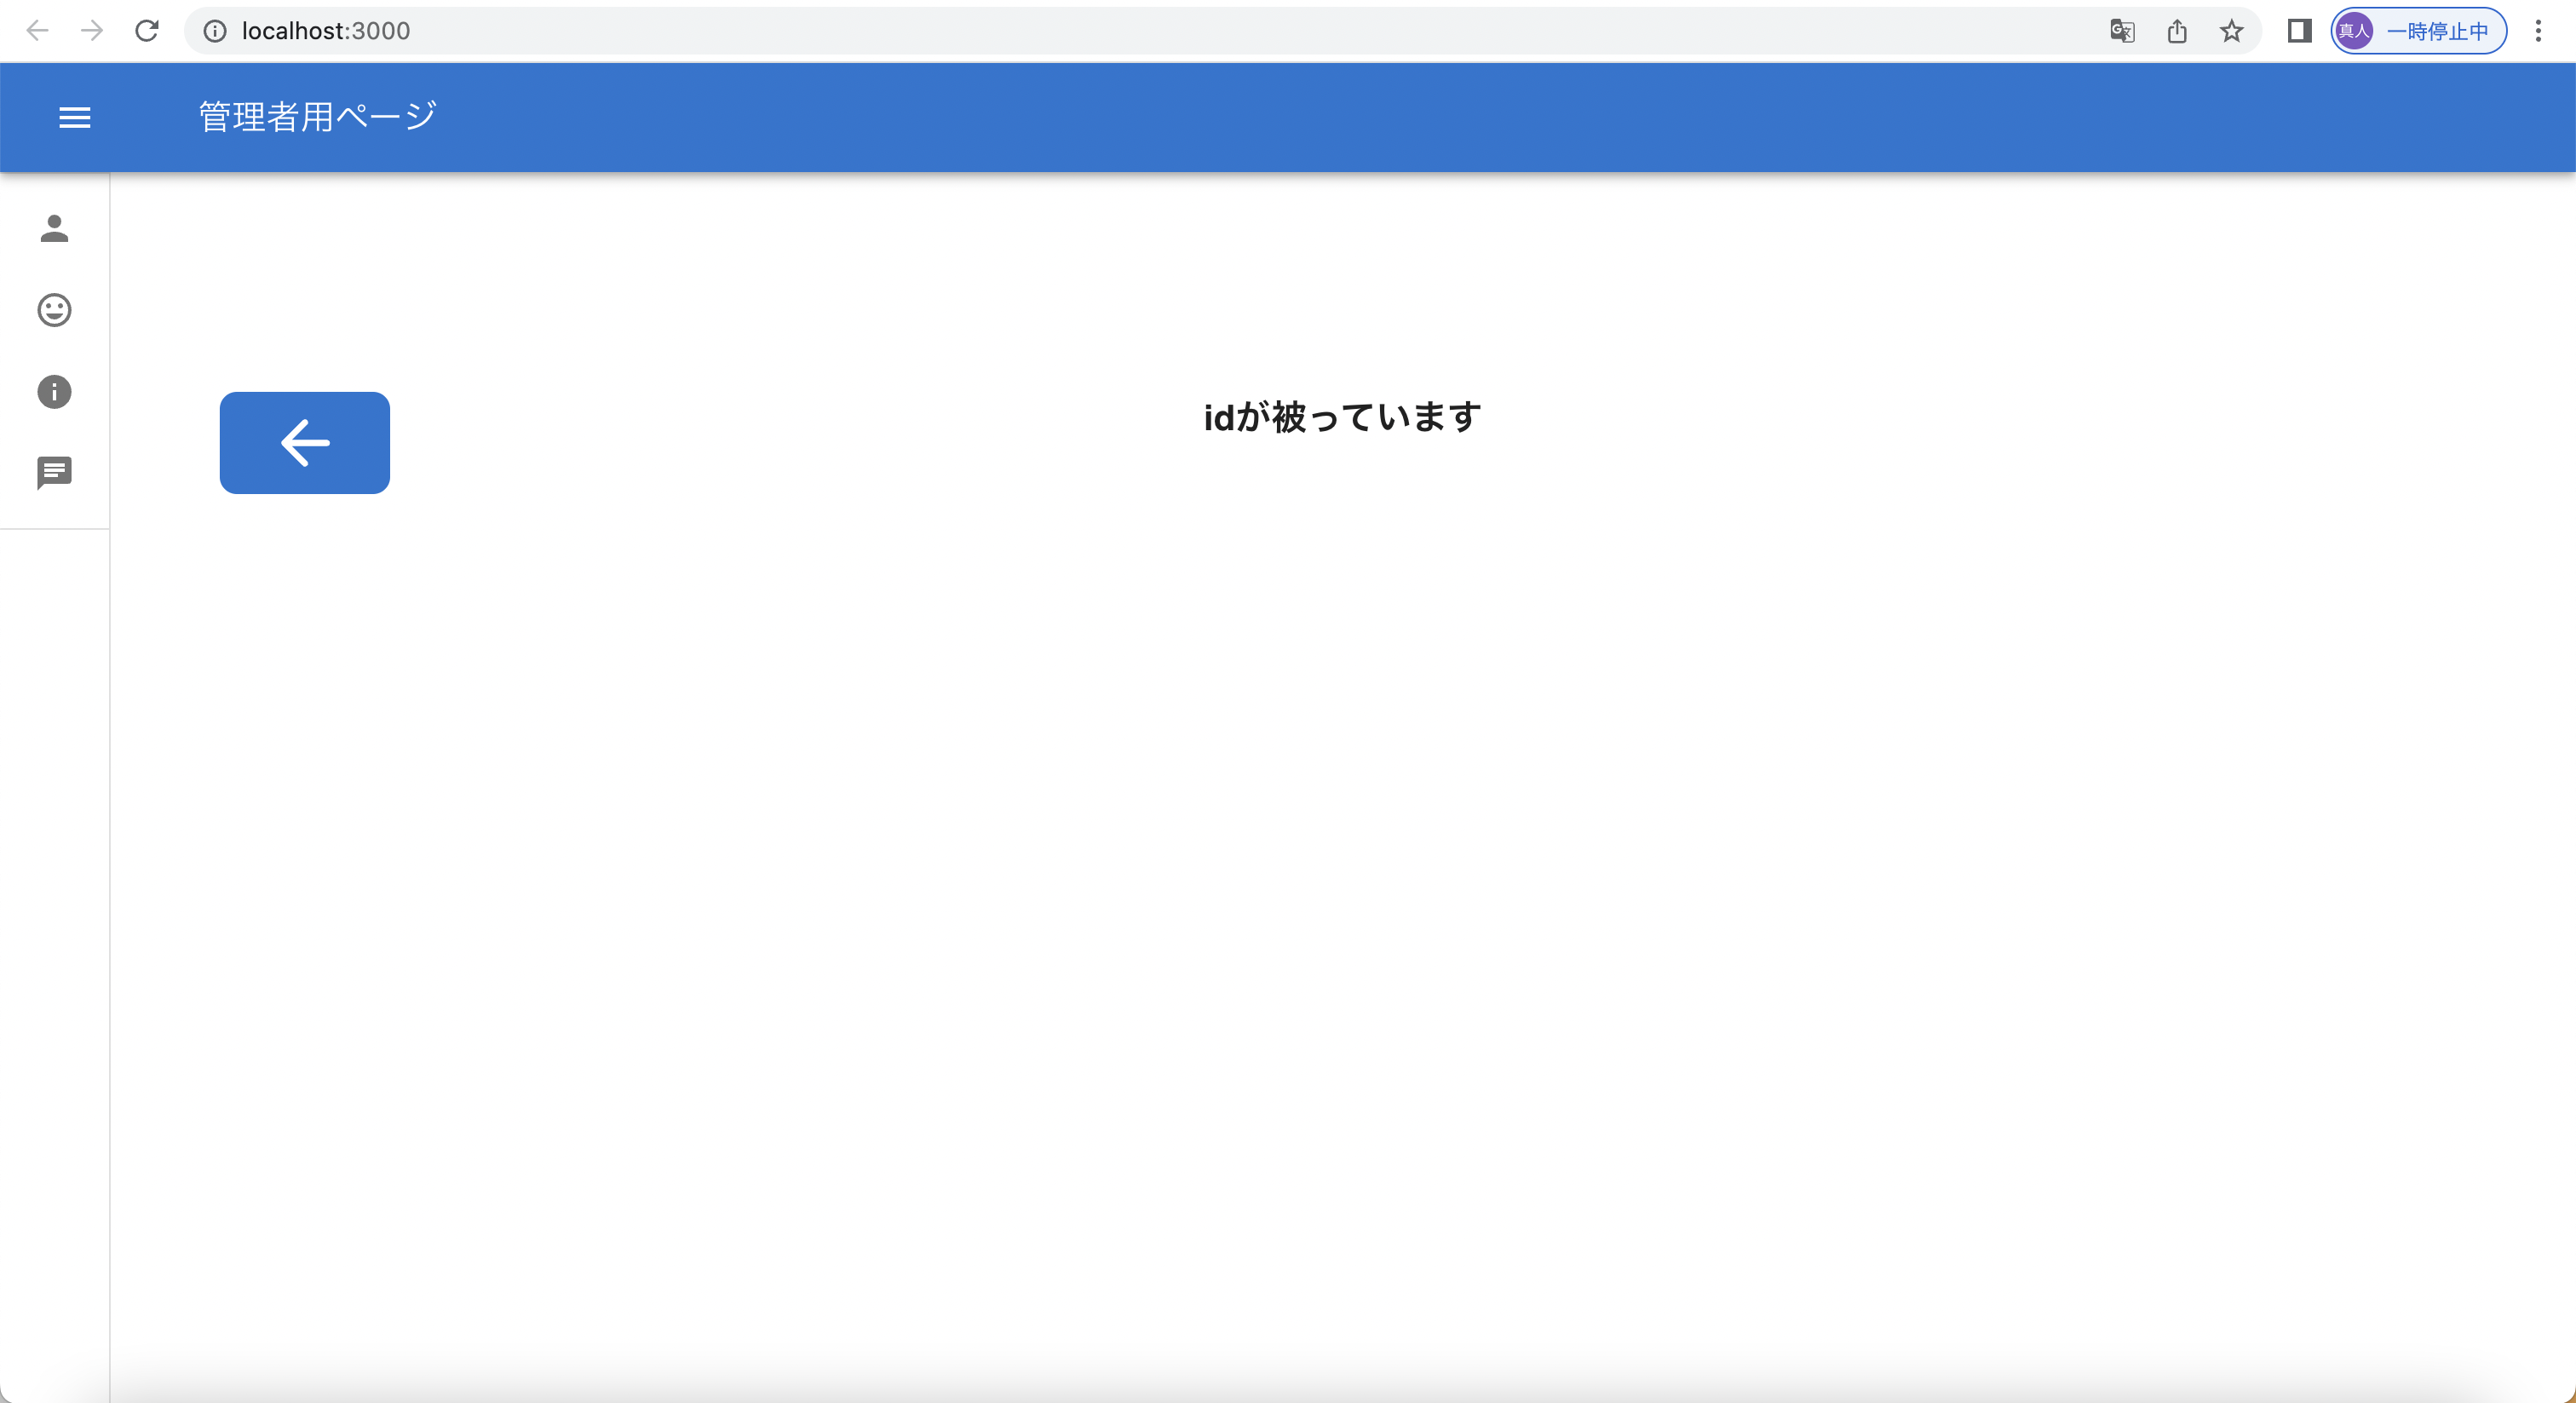
\includegraphics[scale=0.3, clip]{./img/sample8.png}
			\caption{idが被っている際の画面}
			\label{fig:図の名前}
	\end{center}
\end{figure}

\subsection{社員の顔写真閲覧機能}
社員の顔写真を閲覧できるページは図4.6の社員管理画面の詳細ボタンから移動できる.
移動すると過去5日分の写真の笑顔度の傾向に関してのグラフを表示している.
図4.9にそのスクリーンショットを示す.
提出されている写真が一枚も無い,または一枚のみの場合は笑顔度の傾向に関してのグラフを
表示しない様にした(図4.10).
日付のボタンは今日から4日前までの5日分あり,押すとそれぞれの日付で提出された社員の顔写真と
その顔を表情分析したグラフが表示される(図4.11).
もしボタンを押した日付の顔写真が提出されていなかったら図4.12の様になる.

\begin{figure}[!h]
	\begin{center}
			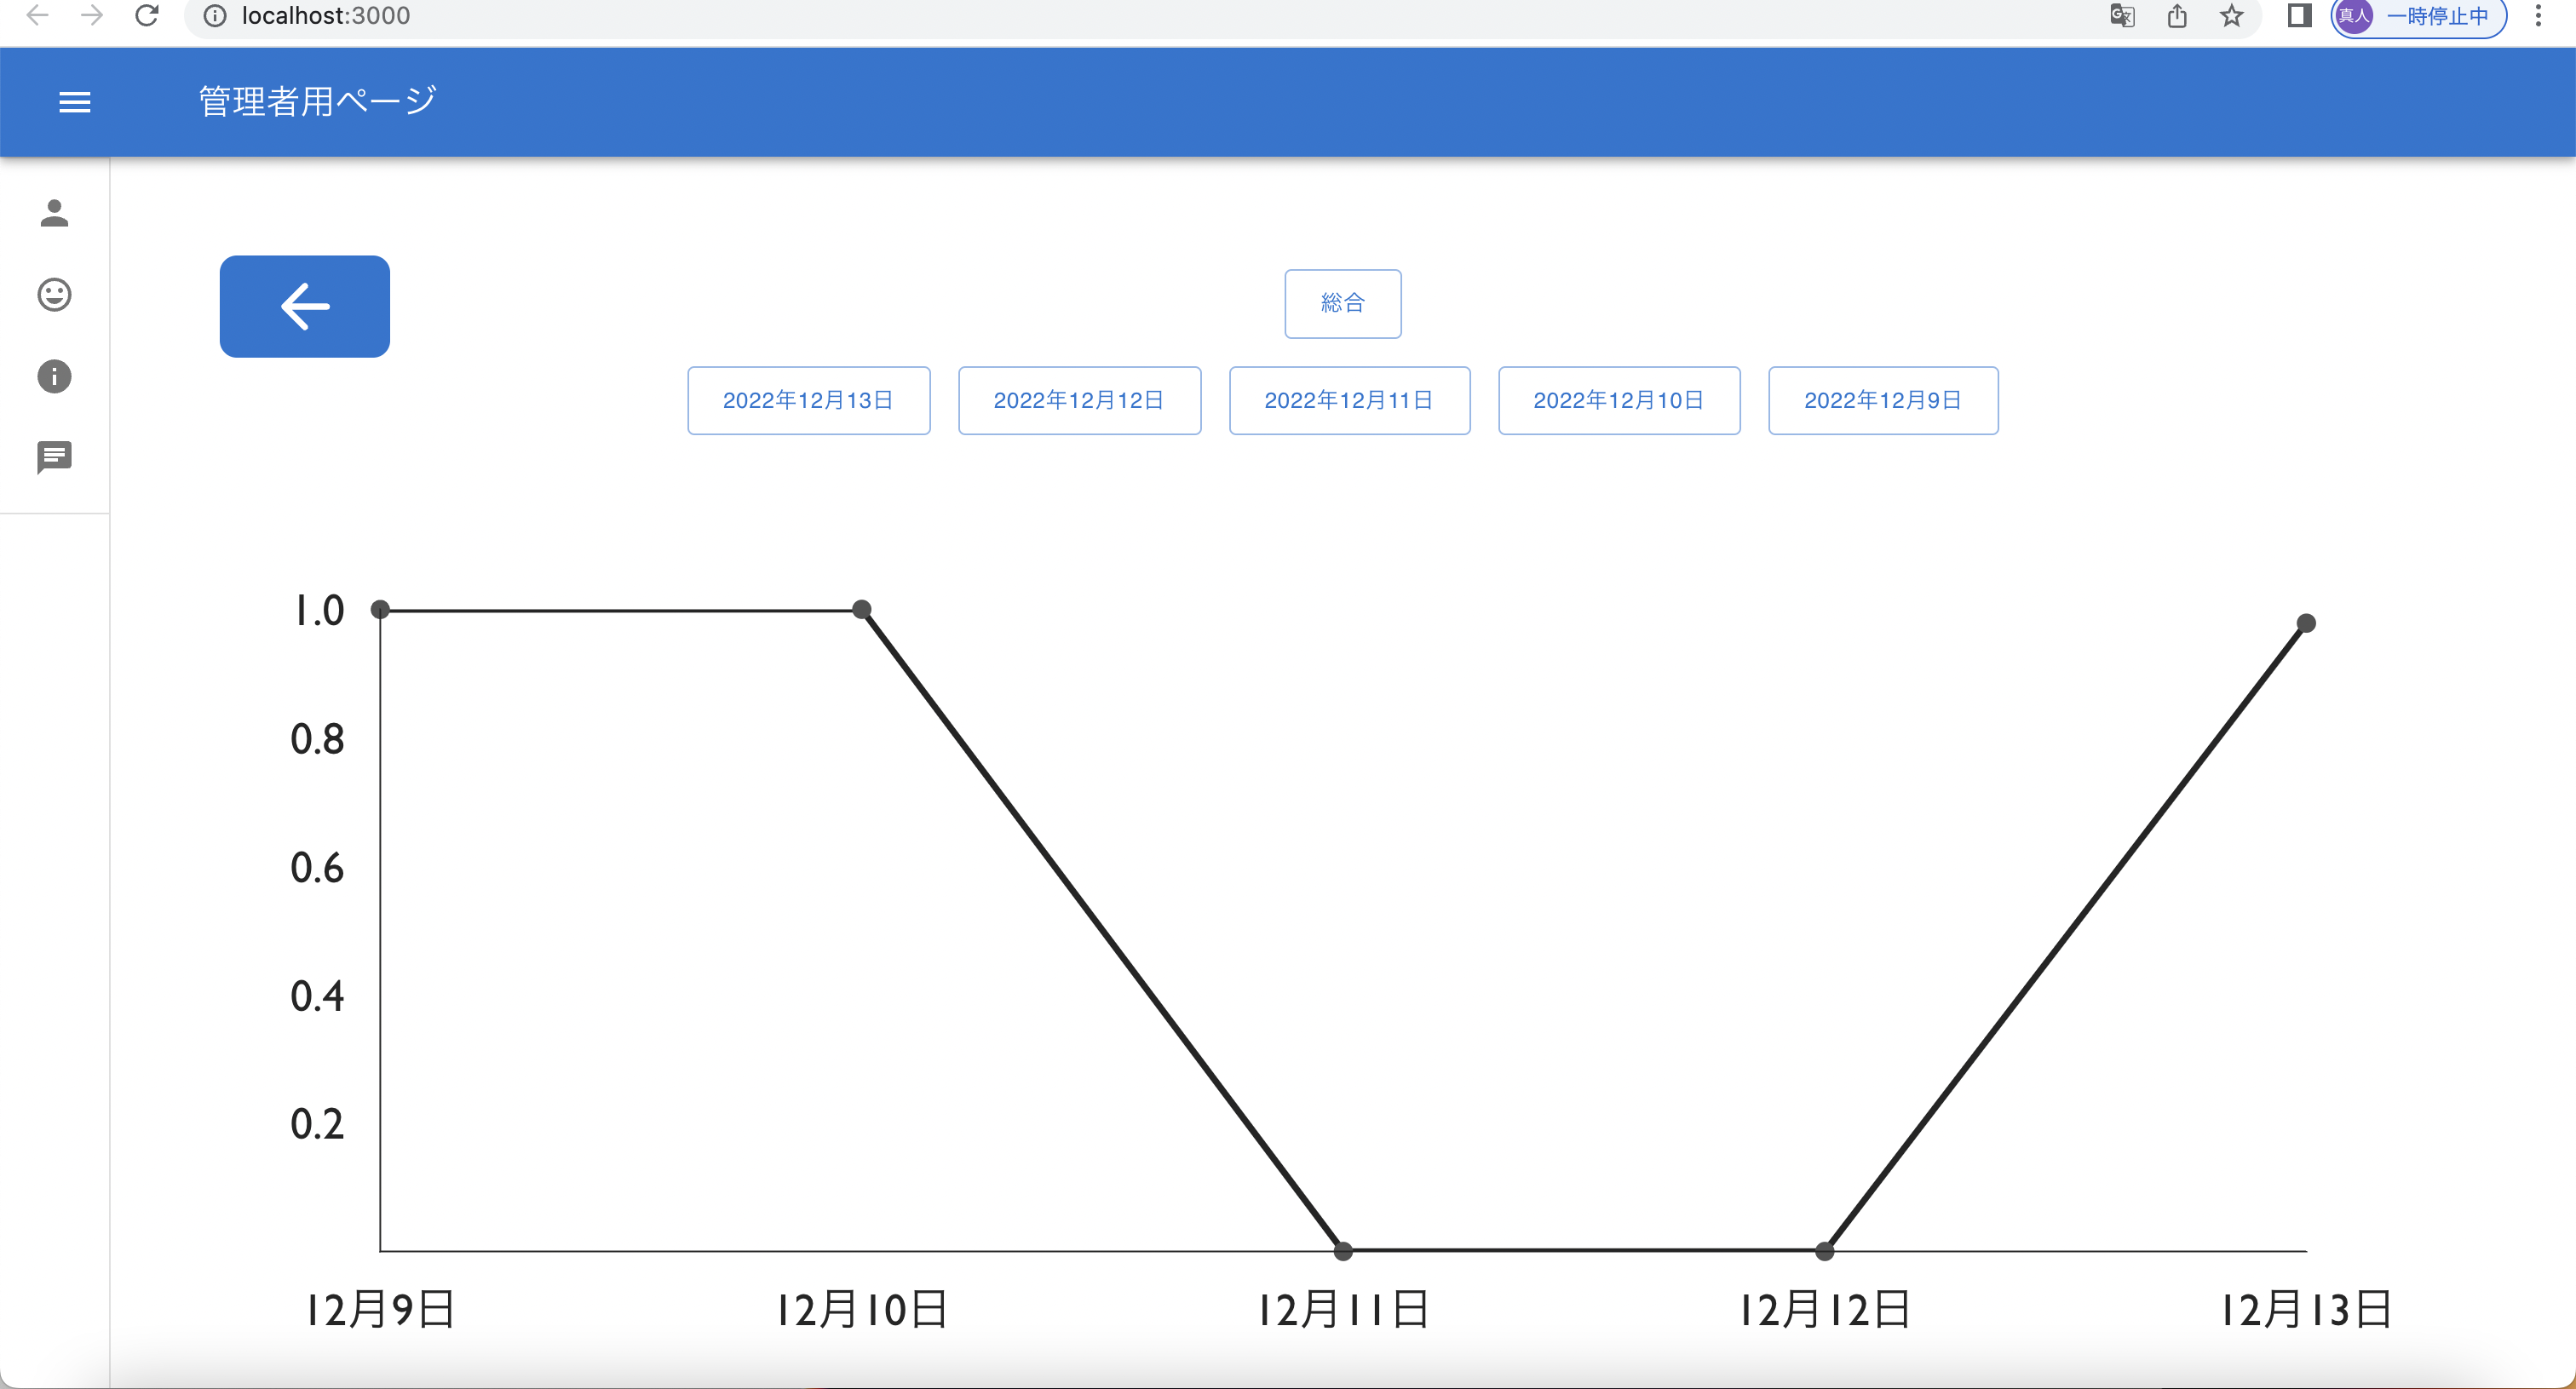
\includegraphics[scale=0.3, clip]{./img/data.png}
			\caption{顔写真閲覧画面}
			\label{fig:図の名前}
	\end{center}
\end{figure}

\begin{figure}[!h]
	\begin{center}
			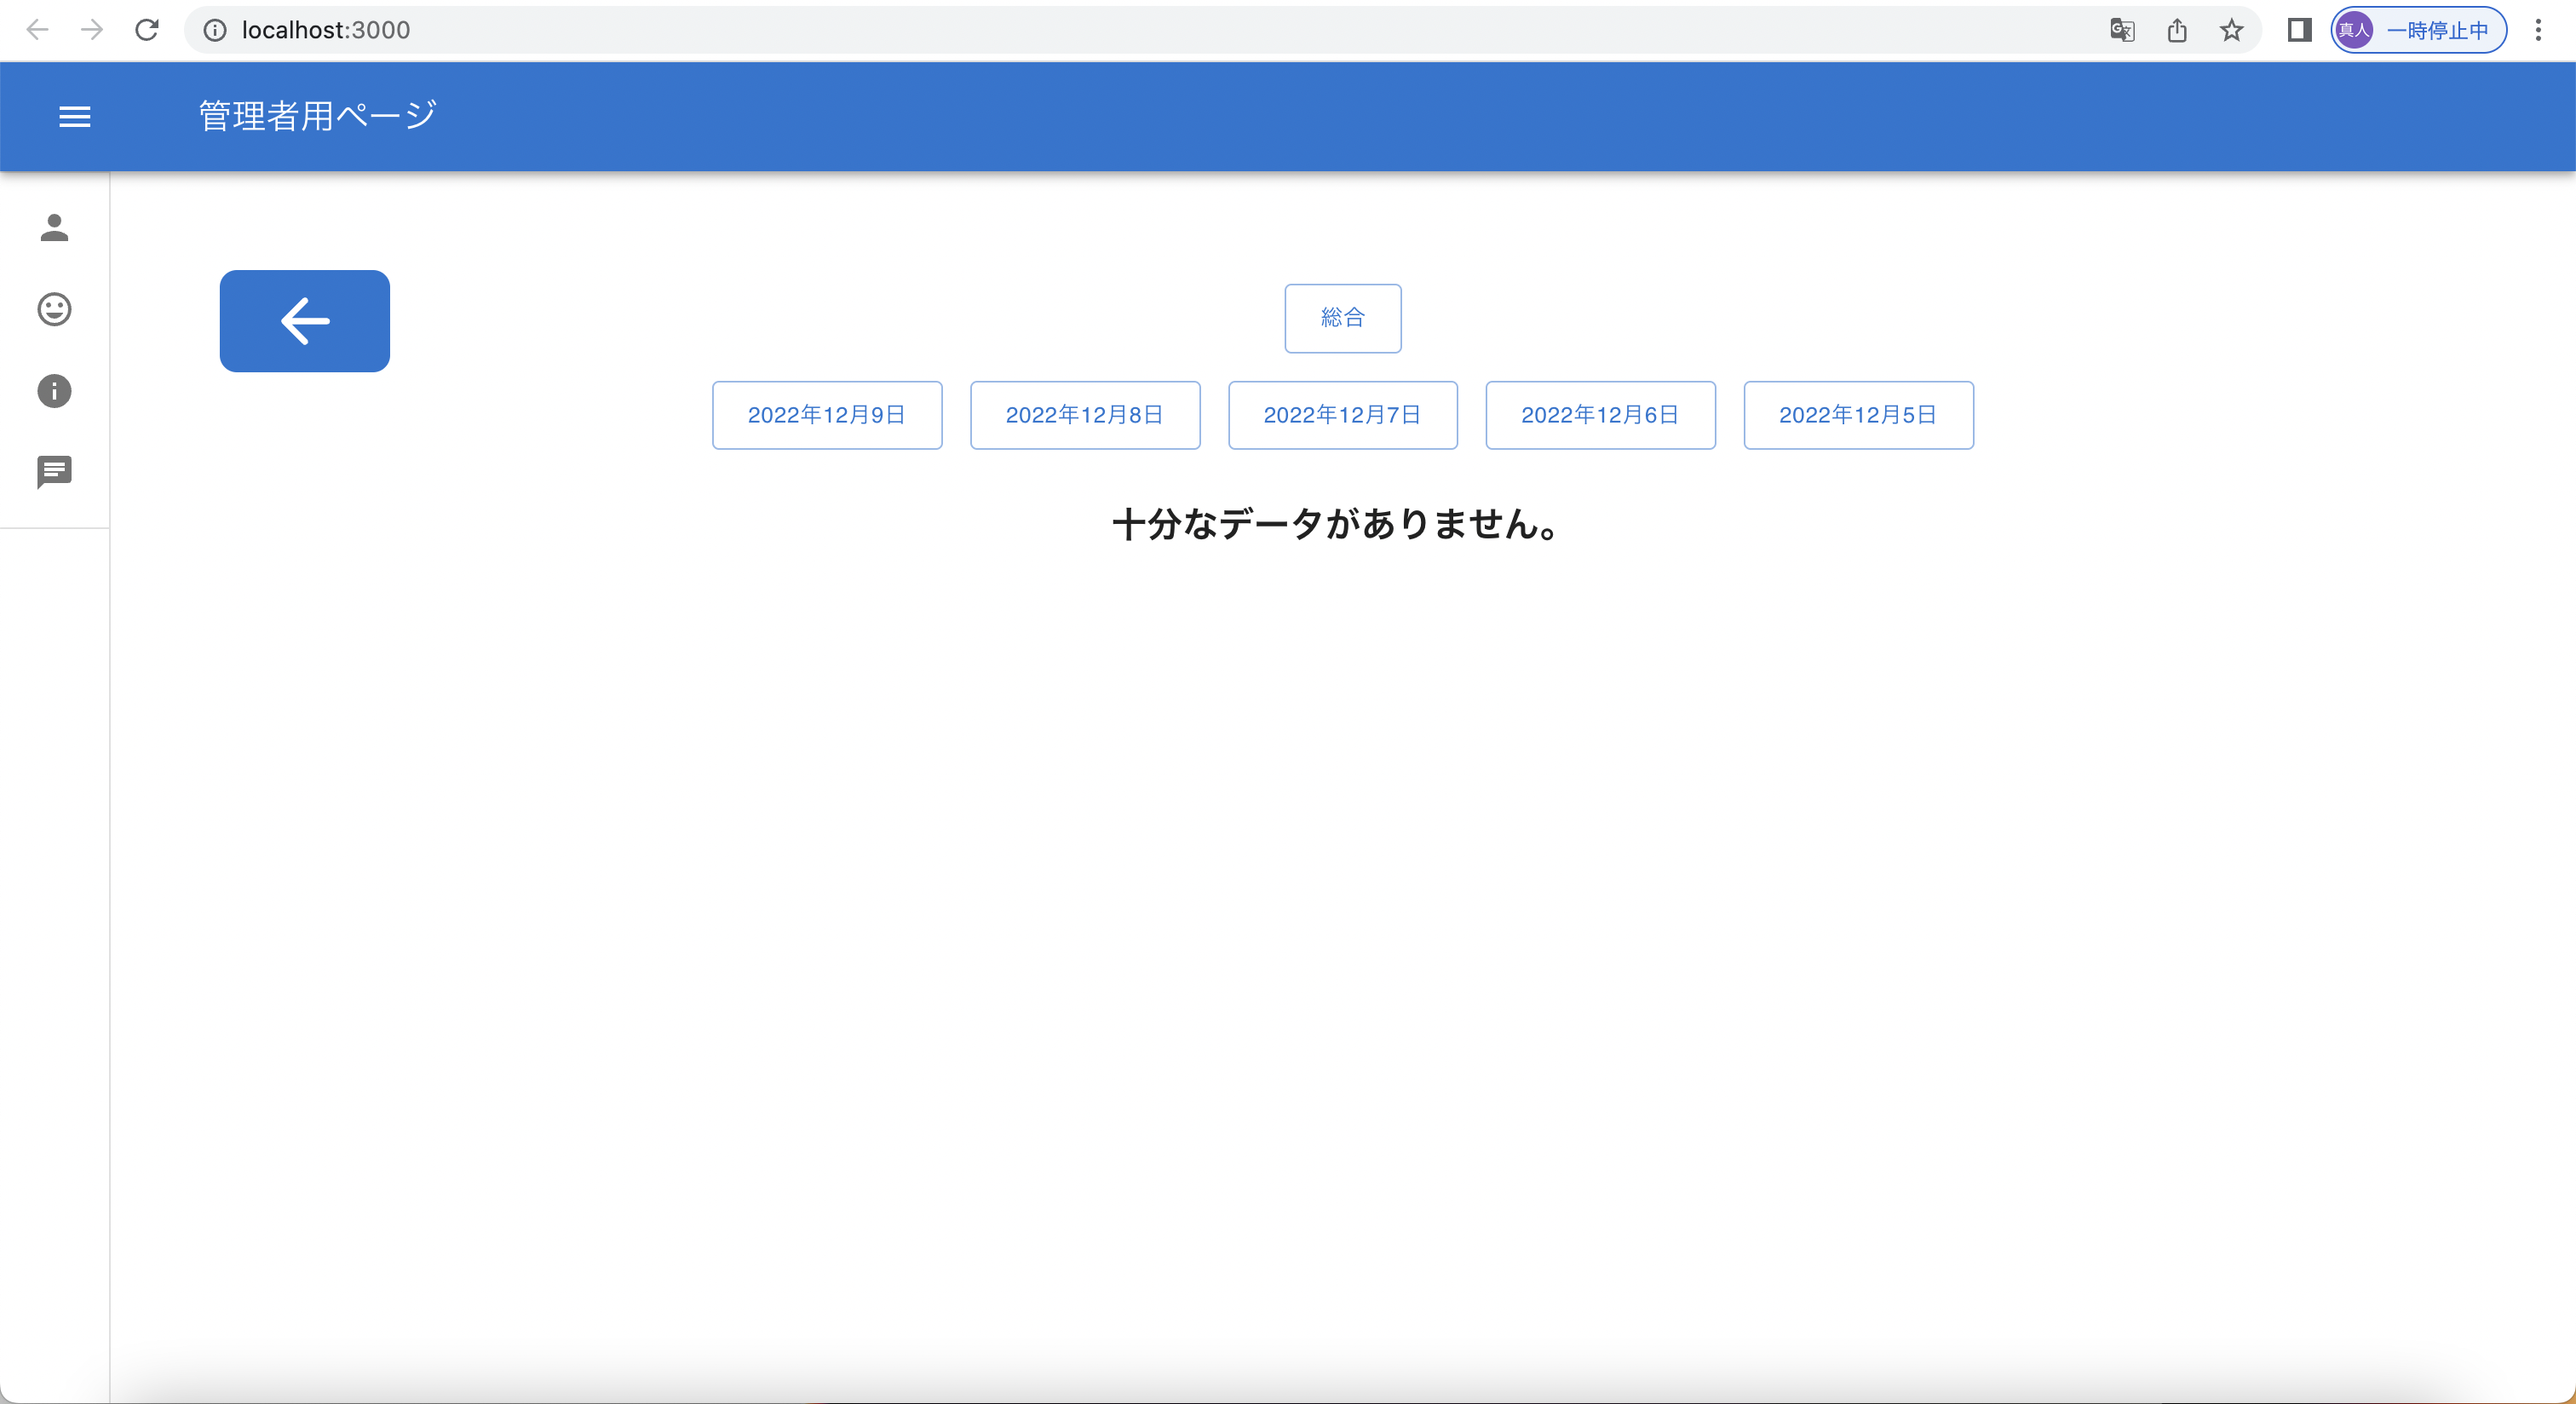
\includegraphics[scale=0.3, clip]{./img/sample9.png}
			\caption{笑顔度傾向グラフ非表示画面}
			\label{fig:図の名前}
	\end{center}
\end{figure}

\clearpage

\begin{figure}[!h]
	\begin{center}
			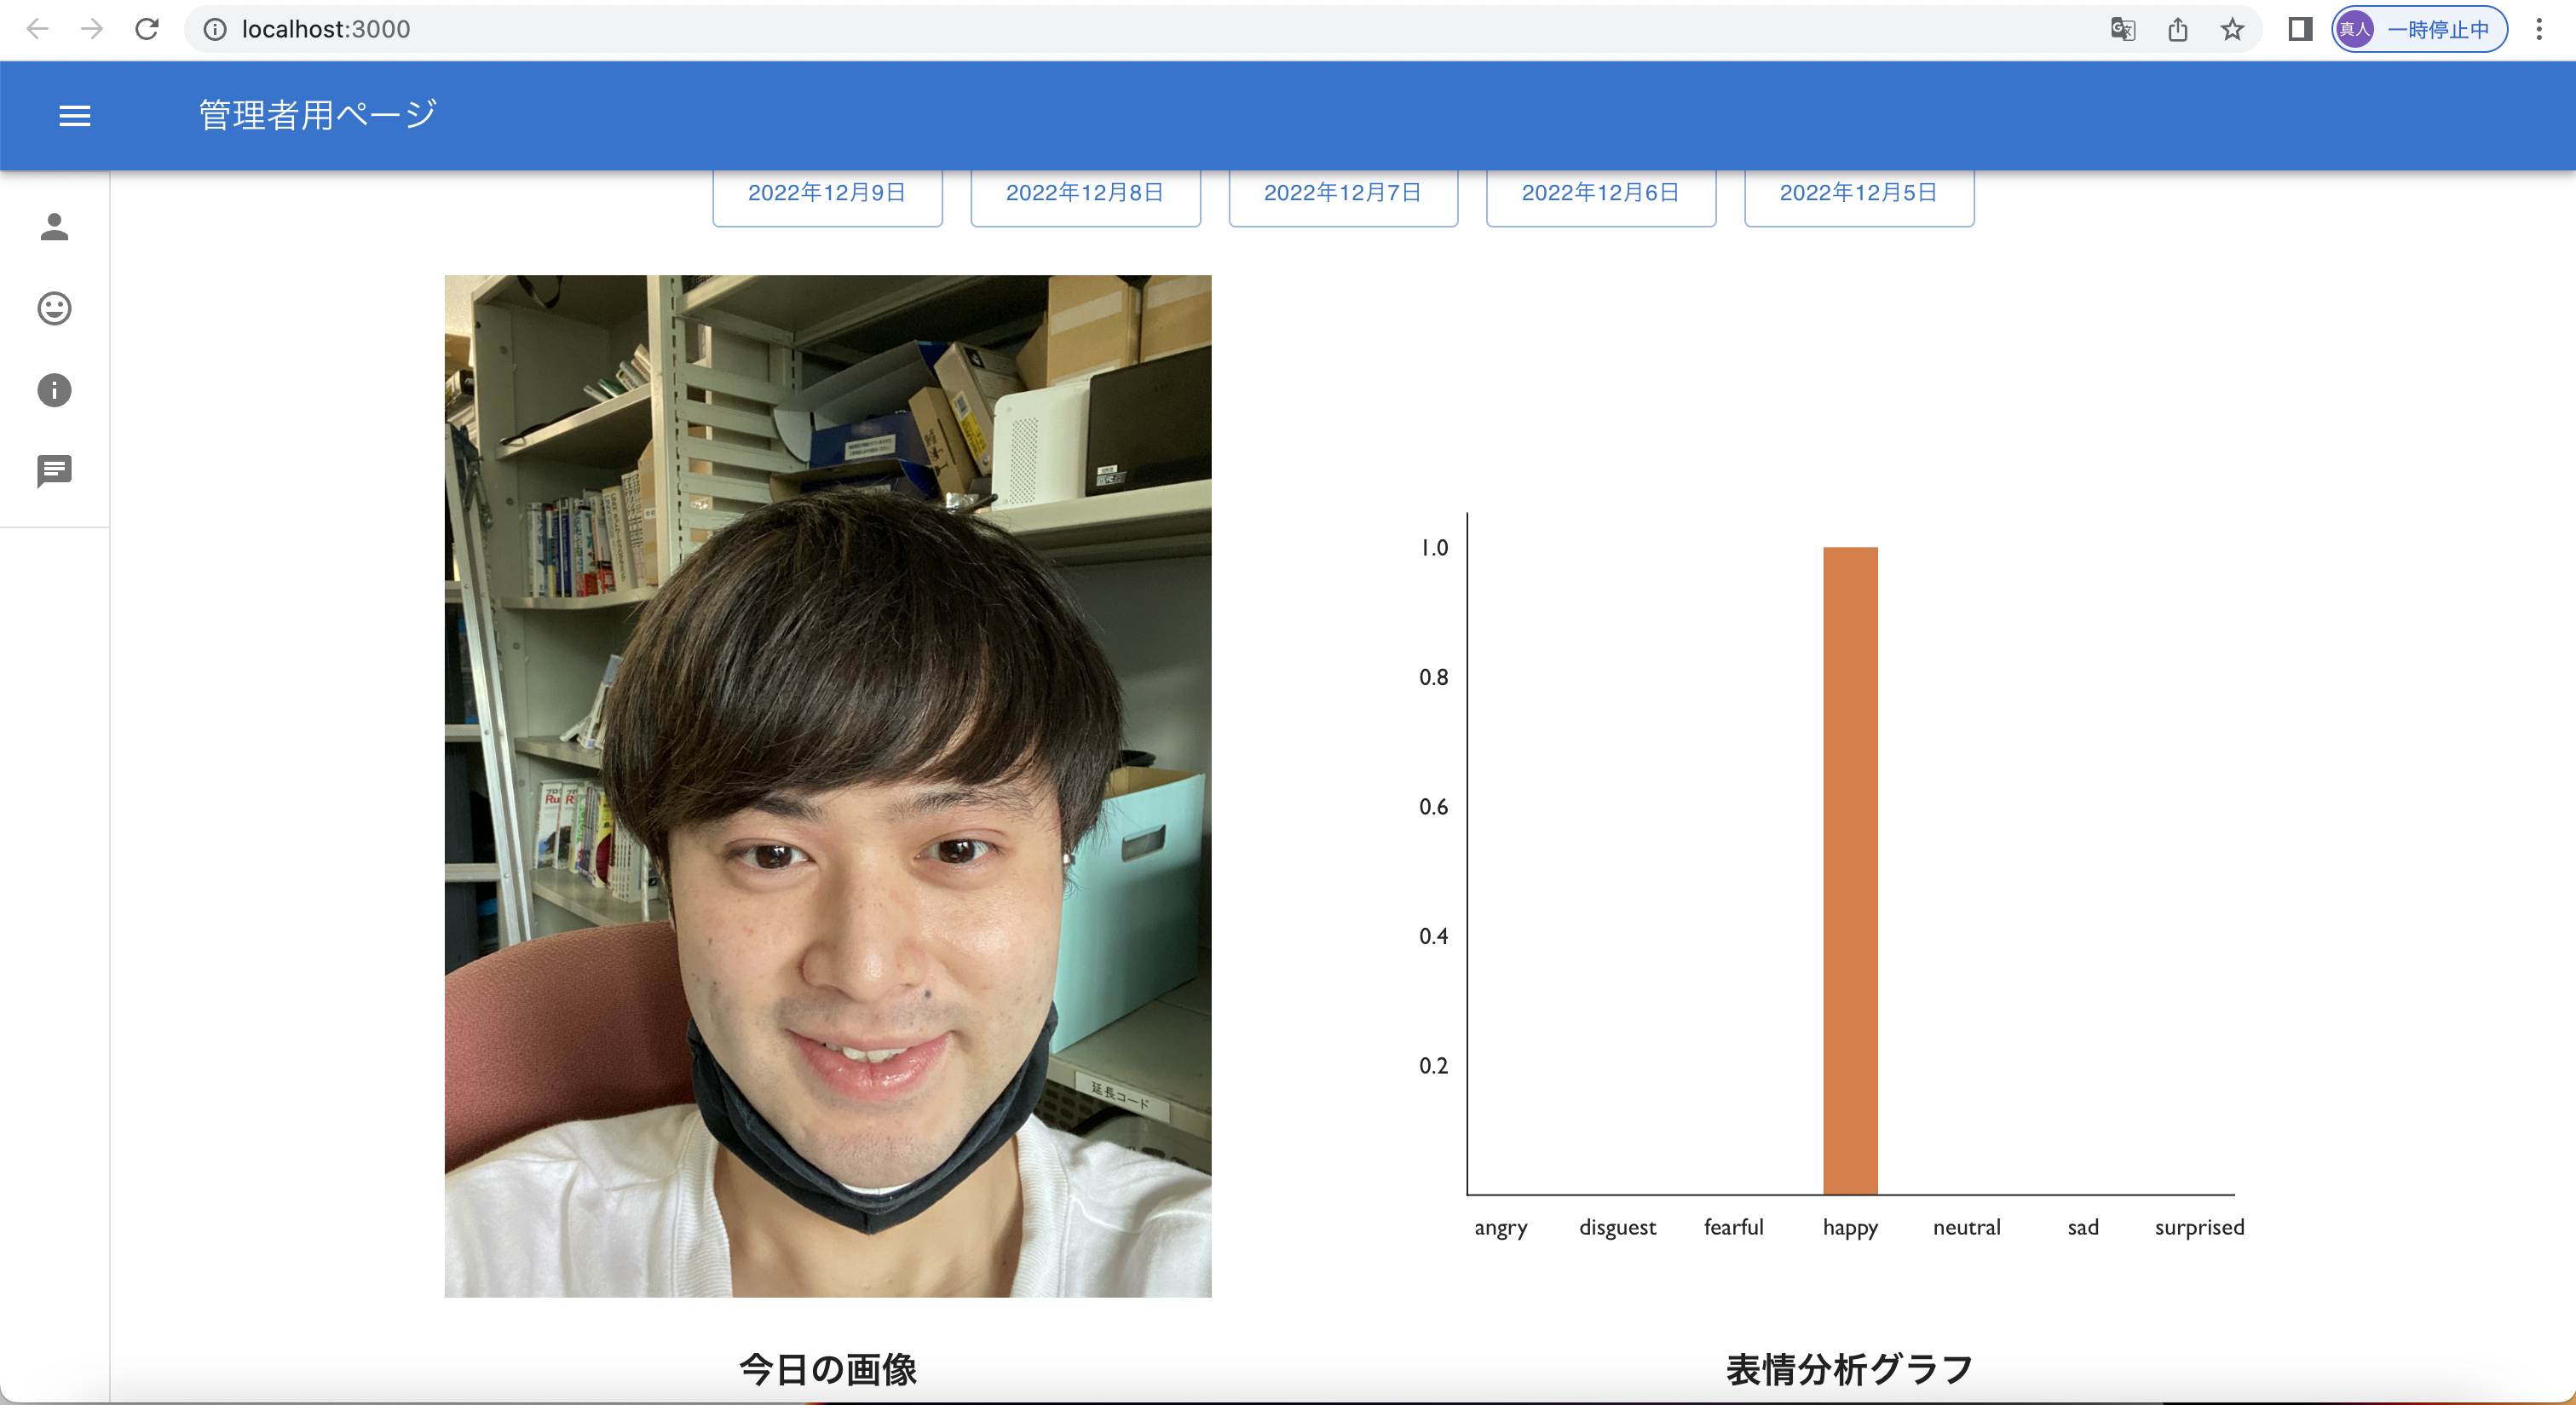
\includegraphics[scale=0.3, clip]{./img/sample10.png}
			\caption{日付のボタンを押した際の画面}
			\label{fig:図の名前}
	\end{center}
\end{figure}

\begin{figure}[!h]
	\begin{center}
			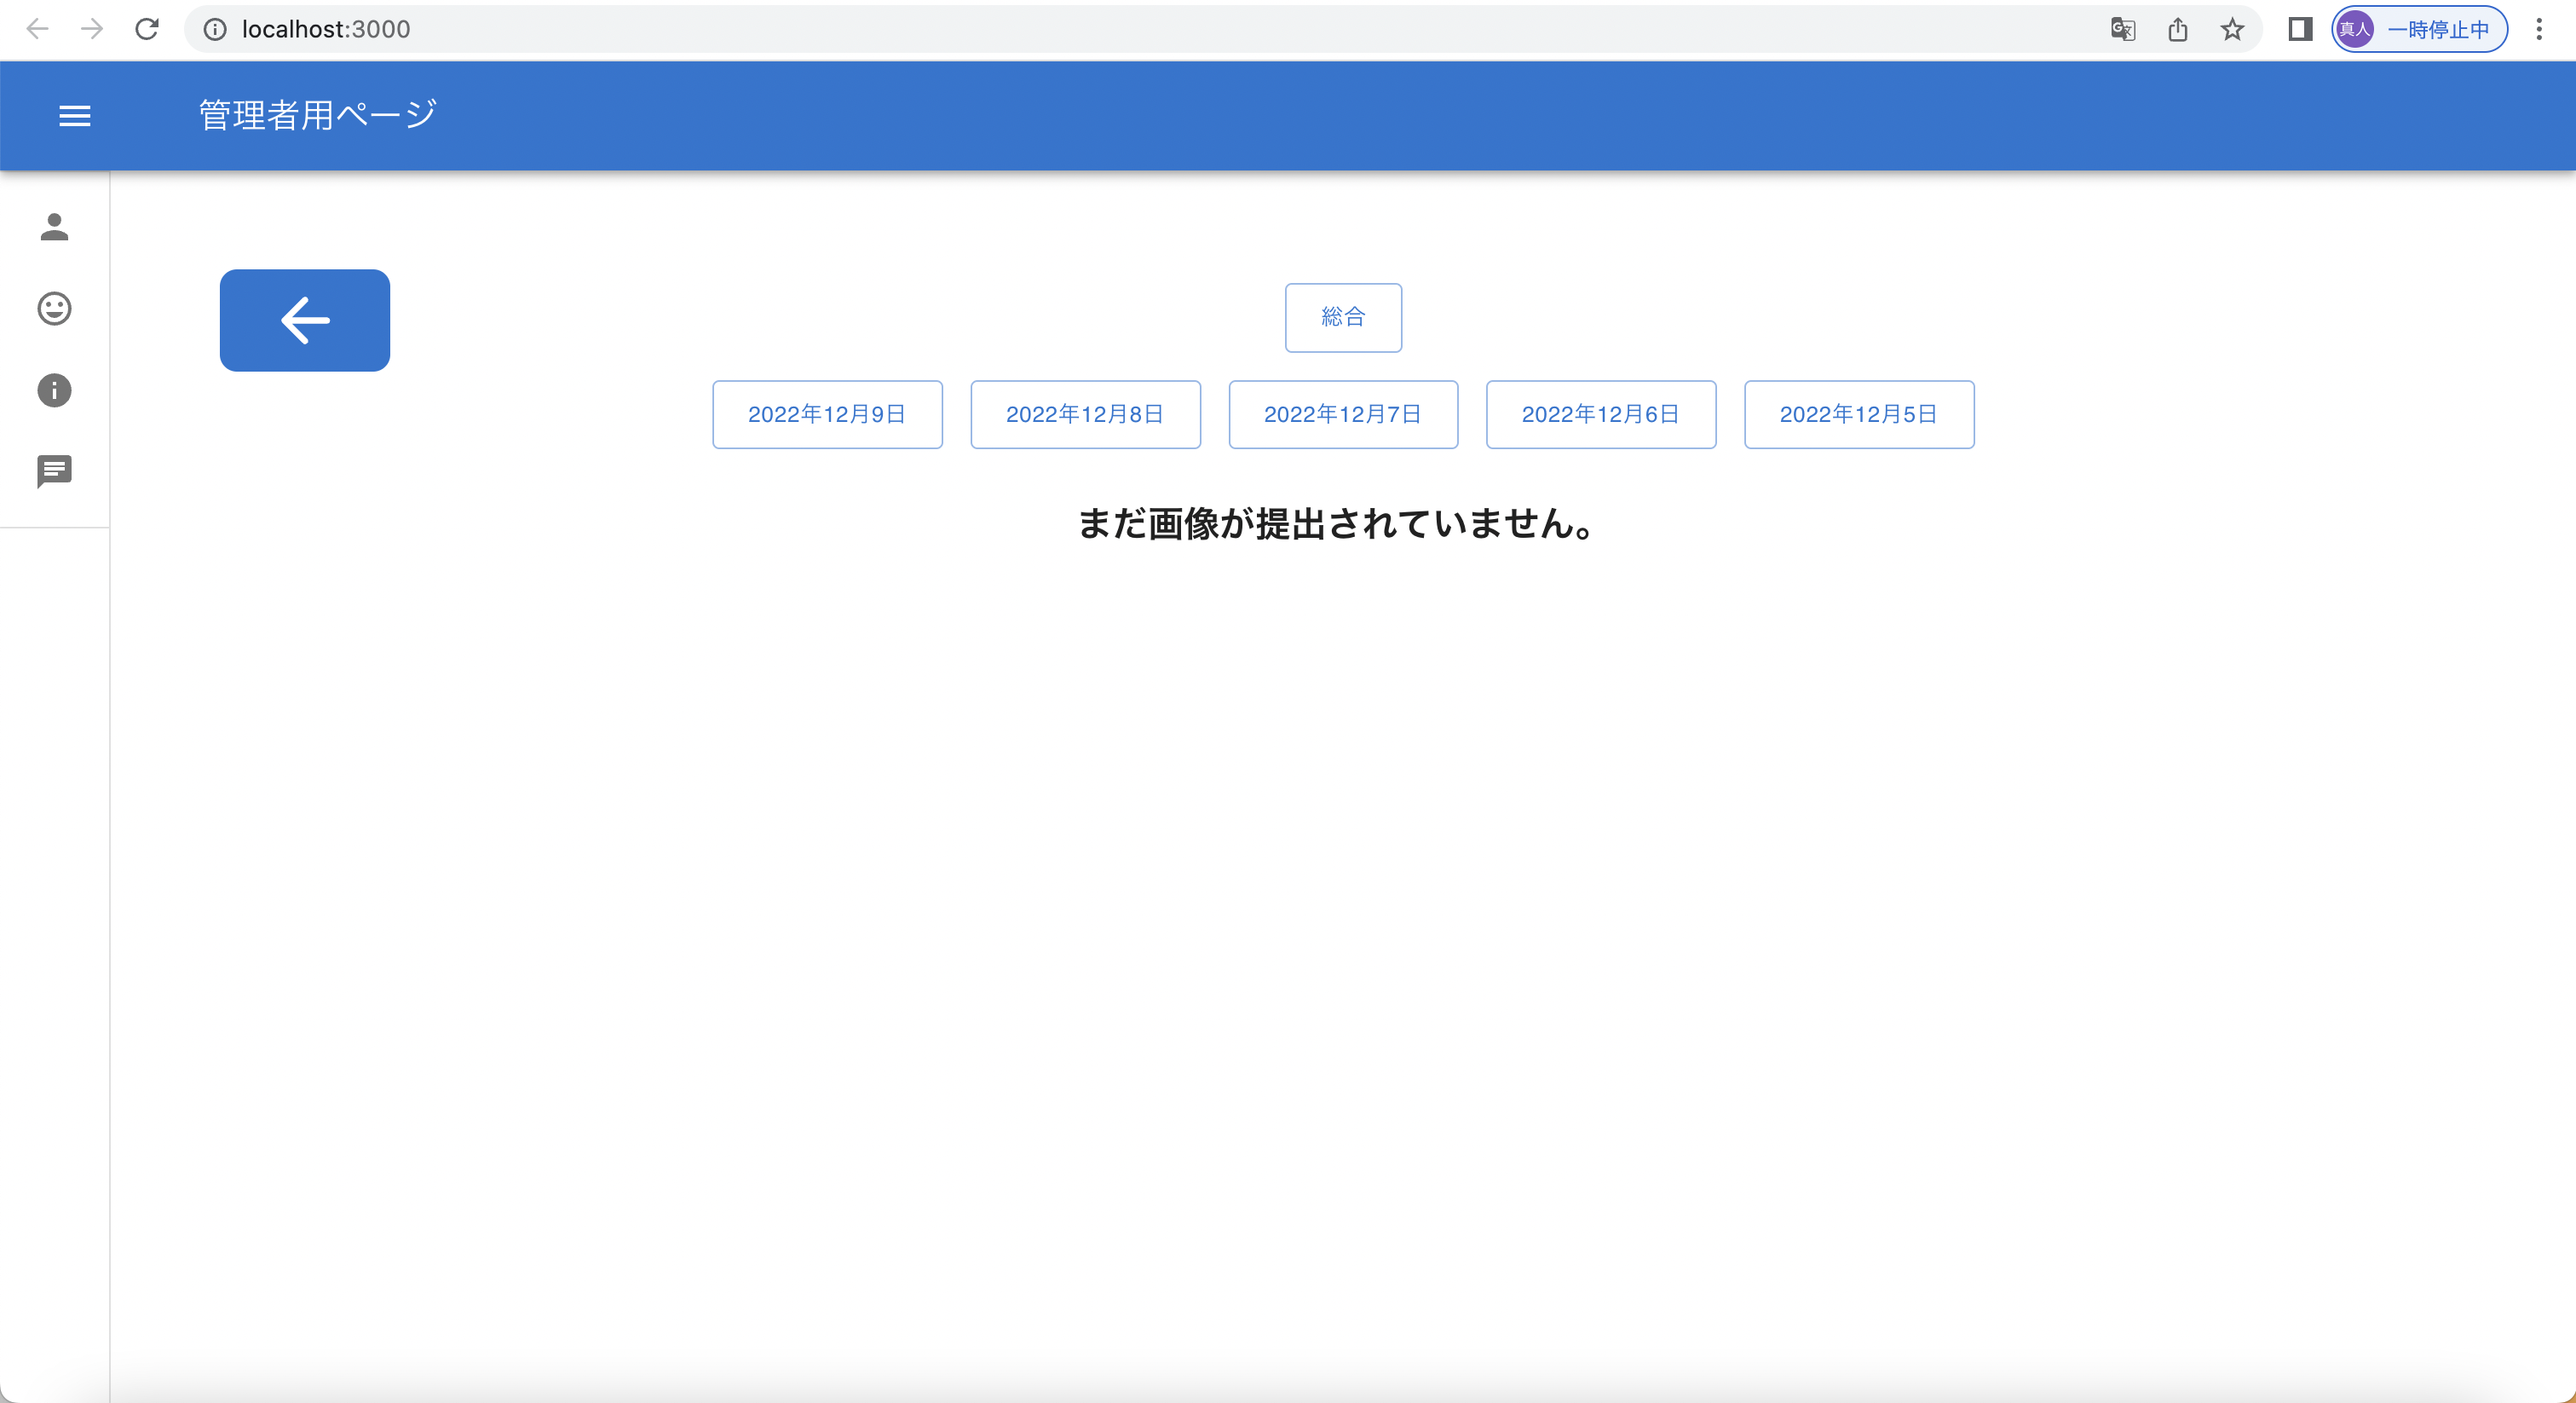
\includegraphics[scale=0.3, clip]{./img/sample11.png}
			\caption{写真が提出されていなかった際の画面}
			\label{fig:図の名前}
	\end{center}
\end{figure}

\clearpage

\section{認証機能}

認証機能はFirebase Authenticationを利用している.今回はユーザーにログインさせる
方法としてGoogleサインインを実装した.
これを利用することによって,アカウント作成といった作業の省略や安全性を提供できる.
ログイン画面のスクリーンショットを図4.13,図4.14に,図4.15にログイン完了画面を示す.
\\

\vspace{17mm}

\begin{figure}[!h]
\begin{center}
  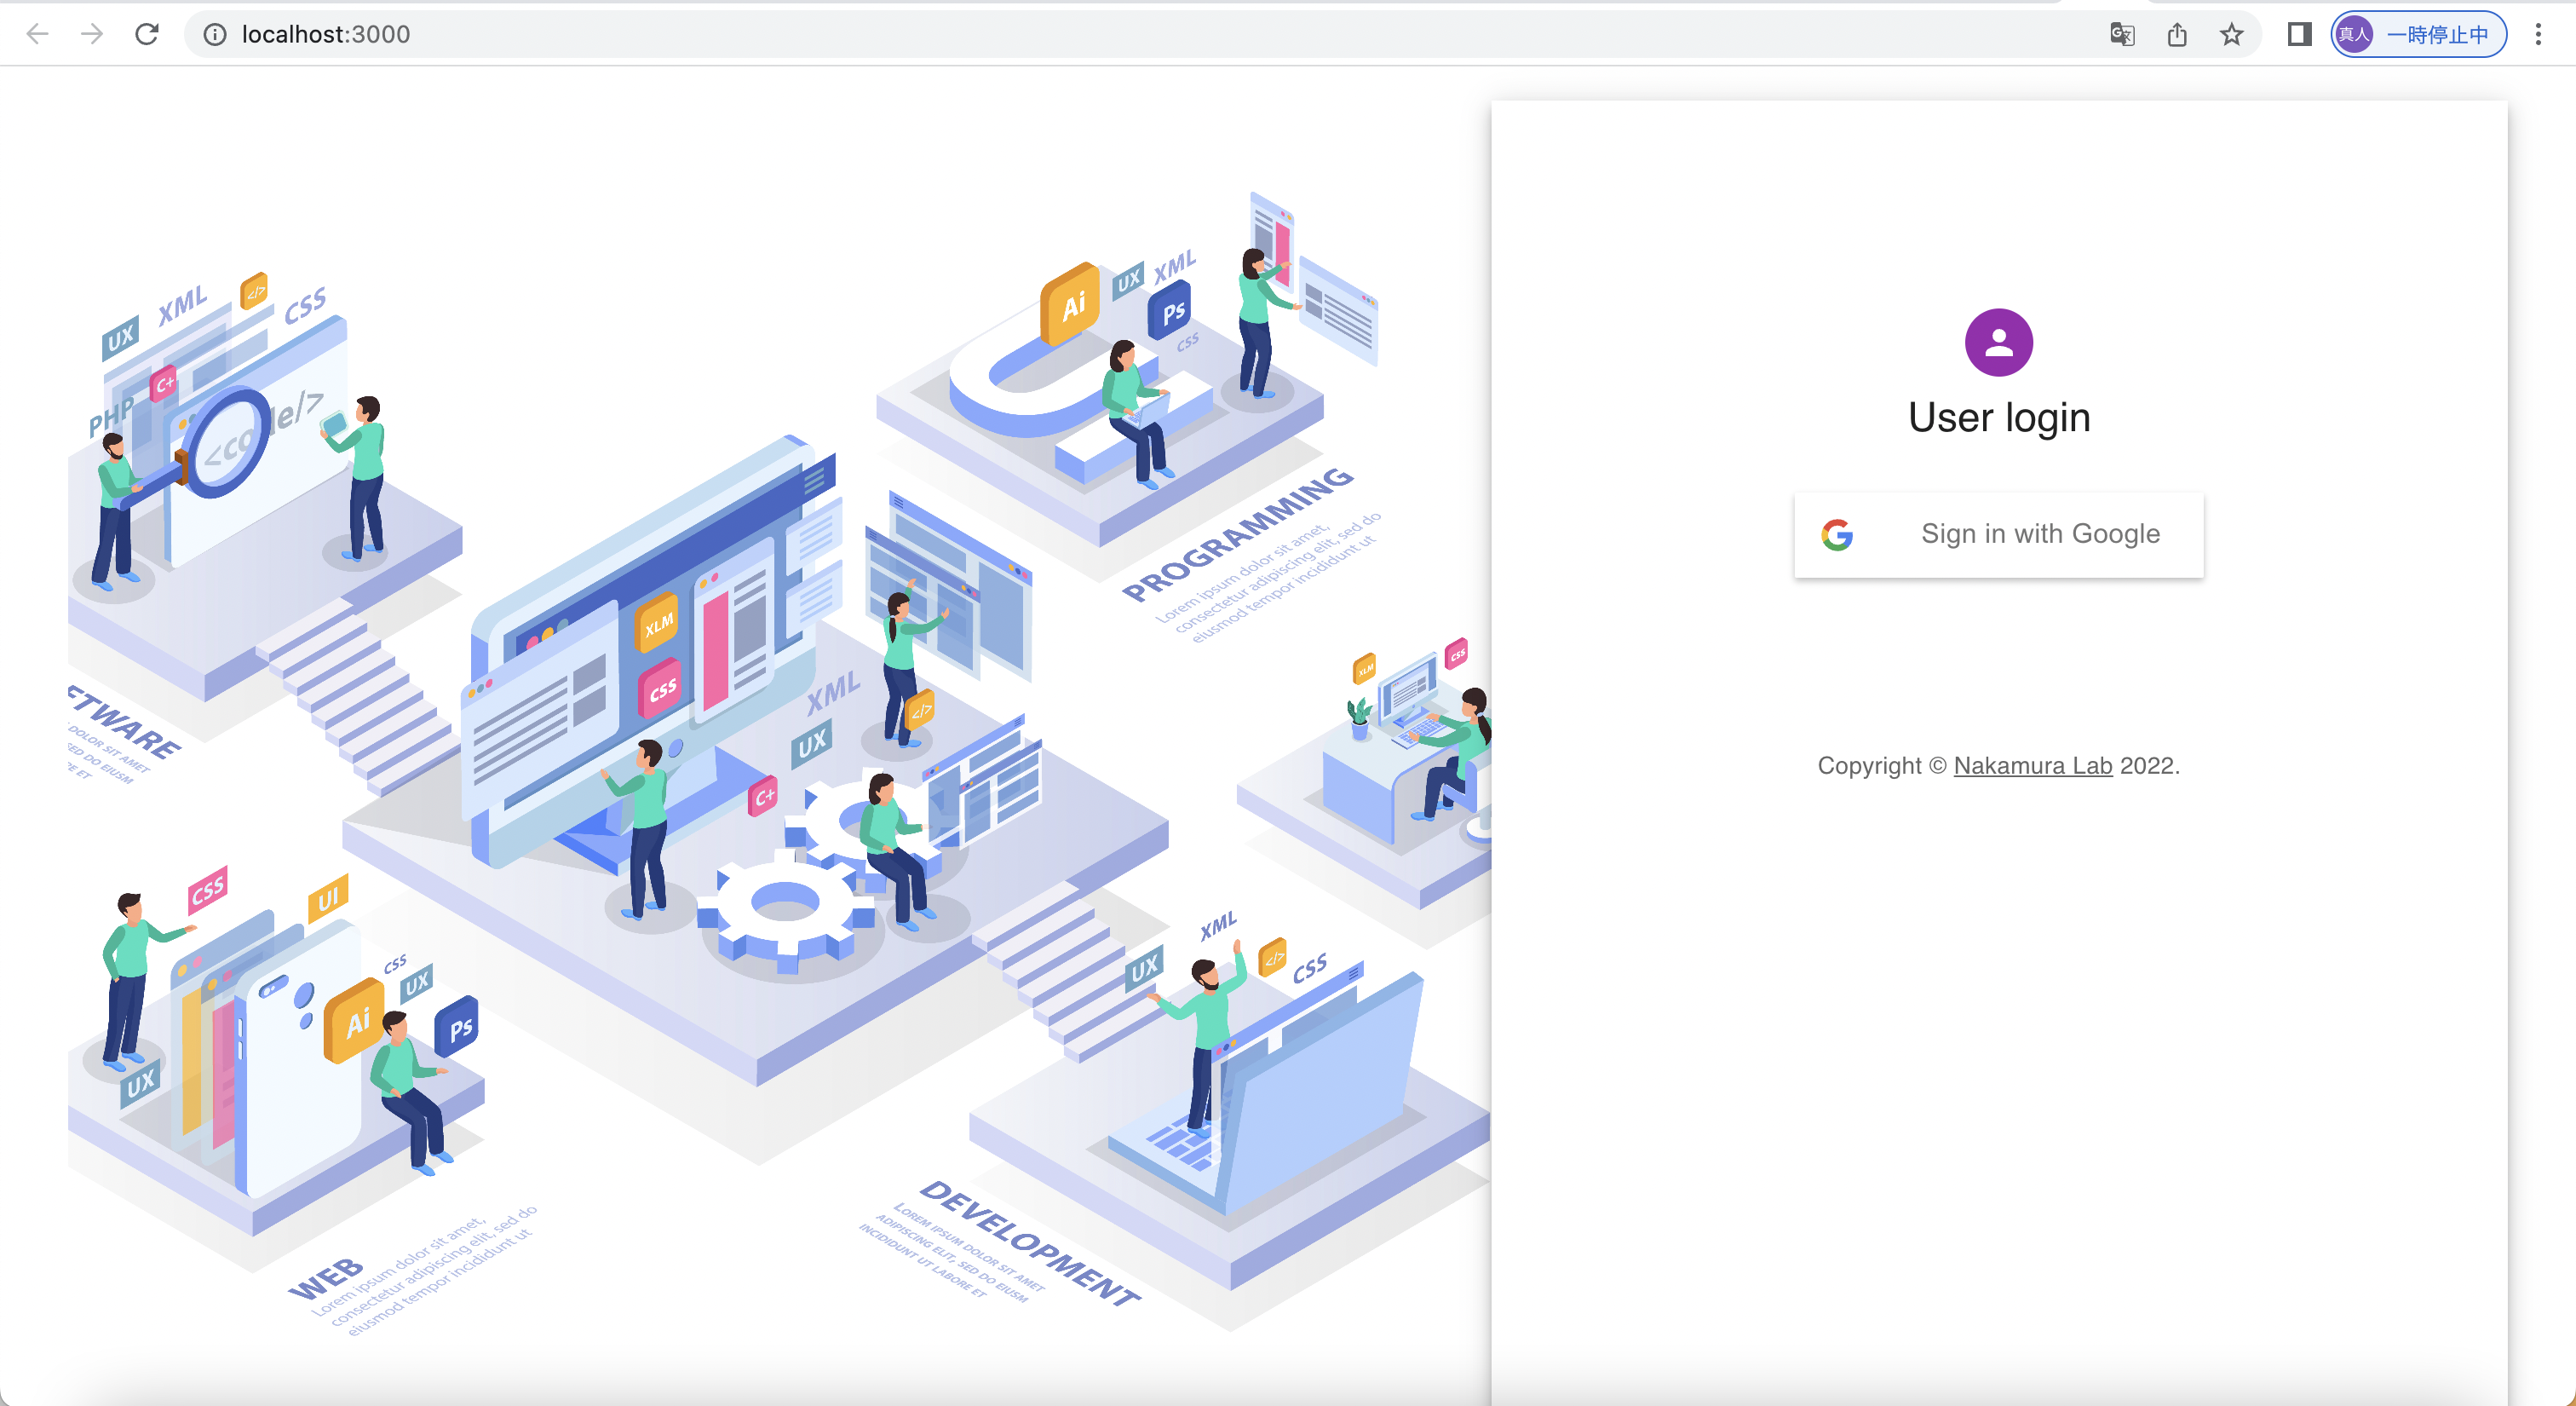
\includegraphics[scale=0.3, clip]{./img/sample13.png}
  \caption{ログイン画面}
  \label{fig:図の名前}
\end{center}
\end{figure}

\begin{figure}[!h]
  \begin{center}
    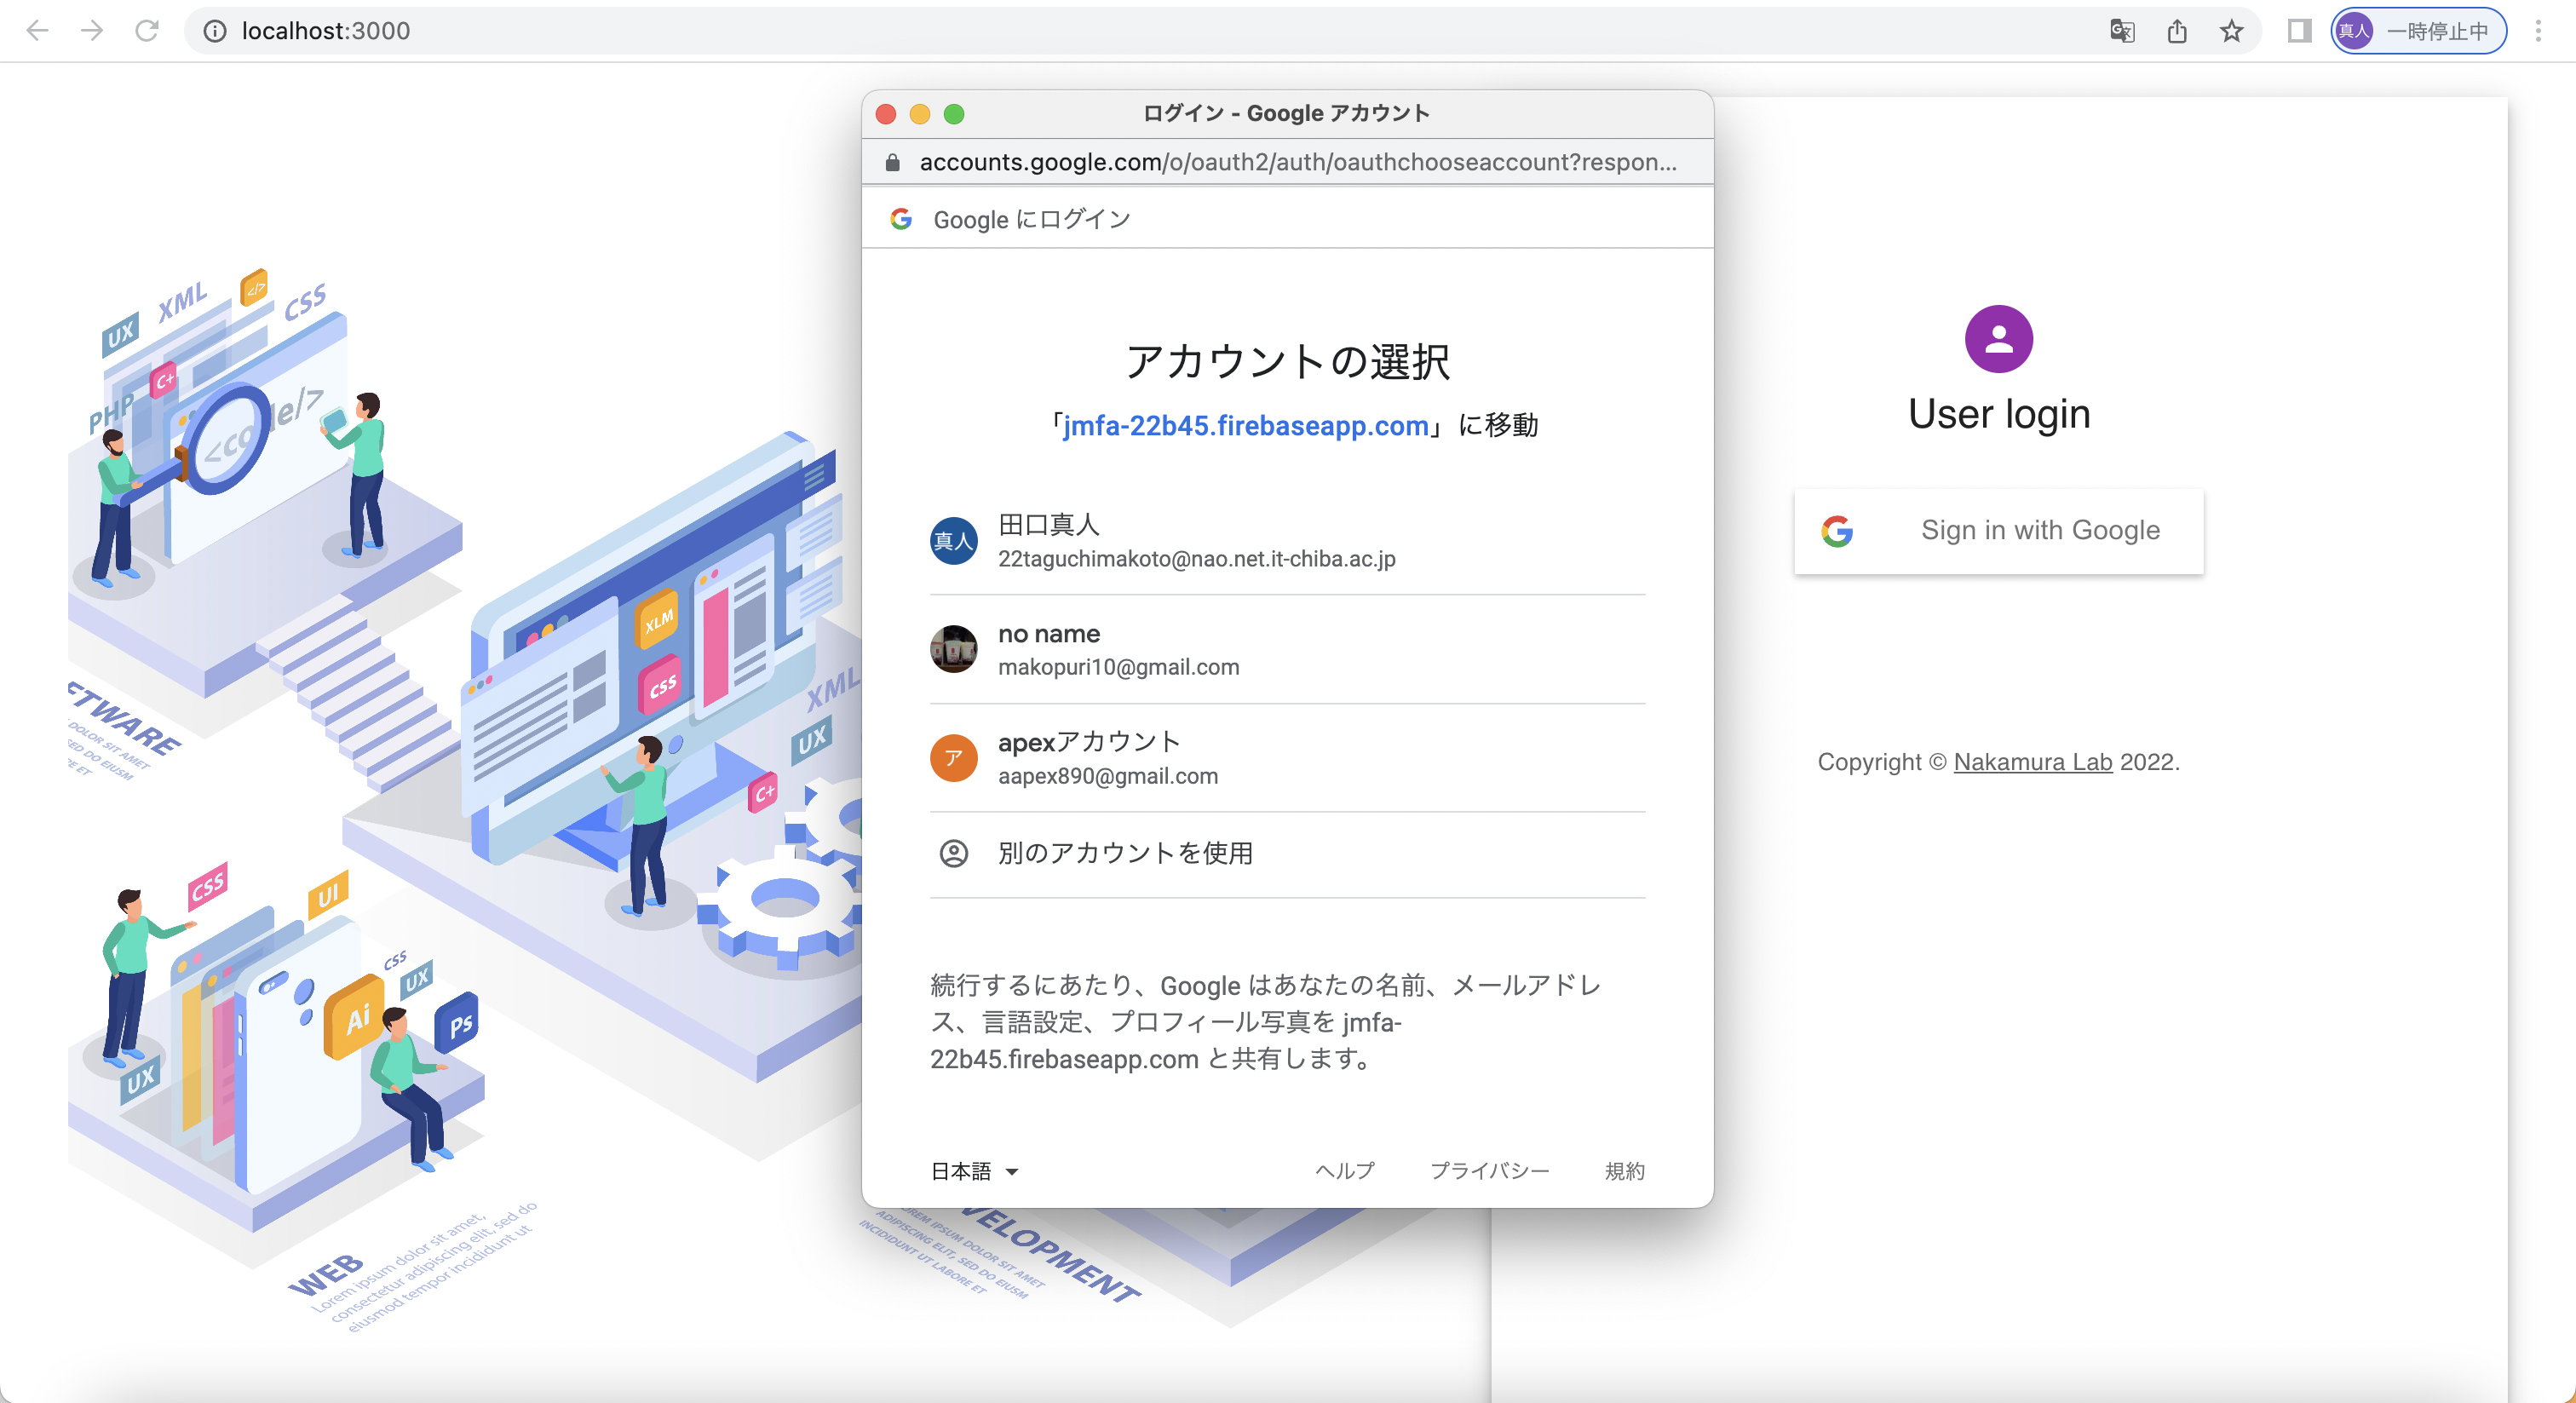
\includegraphics[scale=0.3, clip]{./img/sample14.png}
    \caption{アカウント選択画面}
    \label{fig:図の名前}
  \end{center}
  \end{figure}

  \begin{figure}[!h]
    \begin{center}
      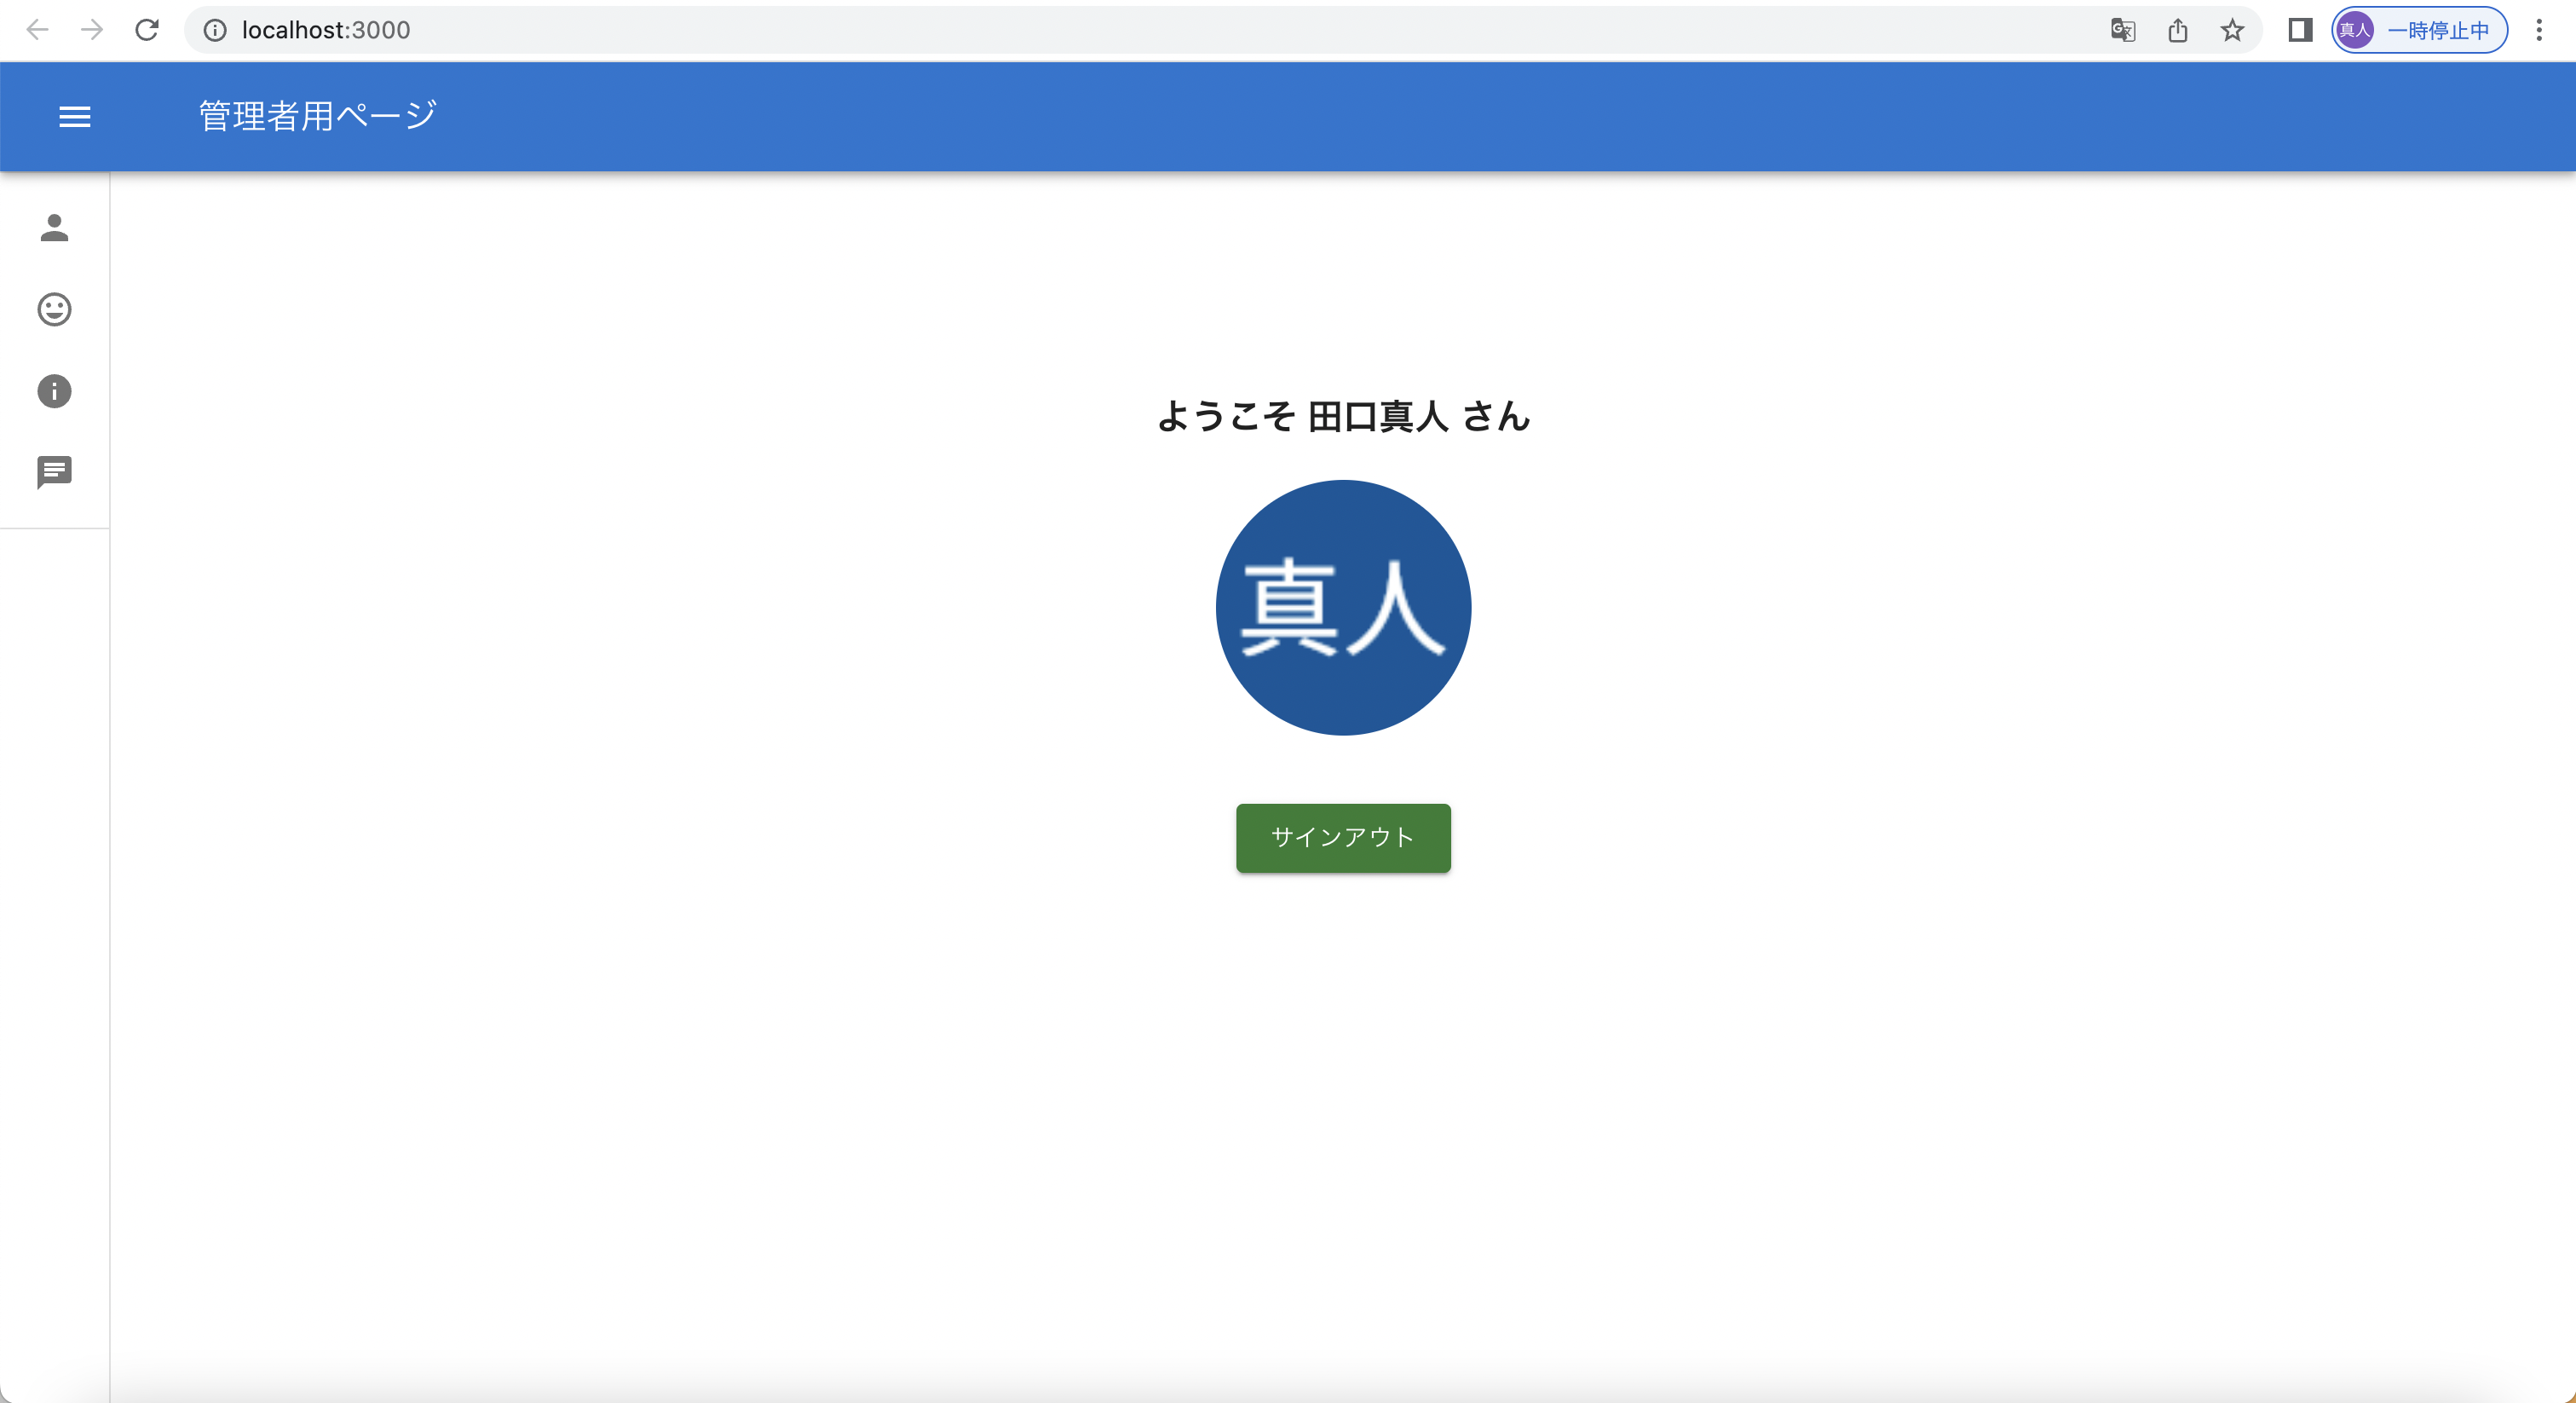
\includegraphics[scale=0.3, clip]{./img/sample15.png}
      \caption{ログイン完了画面}
      \label{fig:図の名前}
    \end{center}
    \end{figure}

    \clearpage

\section{掲示板機能}
管理者が社員全体に通知をする際に用いる機能である.そのため,管理者のみが投稿できる様に
なっており,社員は閲覧のみである.
掲示板機能はmaterial uiにあるライブラリーを利用して作成している.
図4.16は管理者ページから見た掲示板画面,図4.17は管理者が文字を入力している画面,
図4.18は入力した文字を投稿した画面,図4.19は社員ページから見た掲示板画面を示している.

\vspace{30mm}

\begin{figure}[!h]
  \begin{center}
    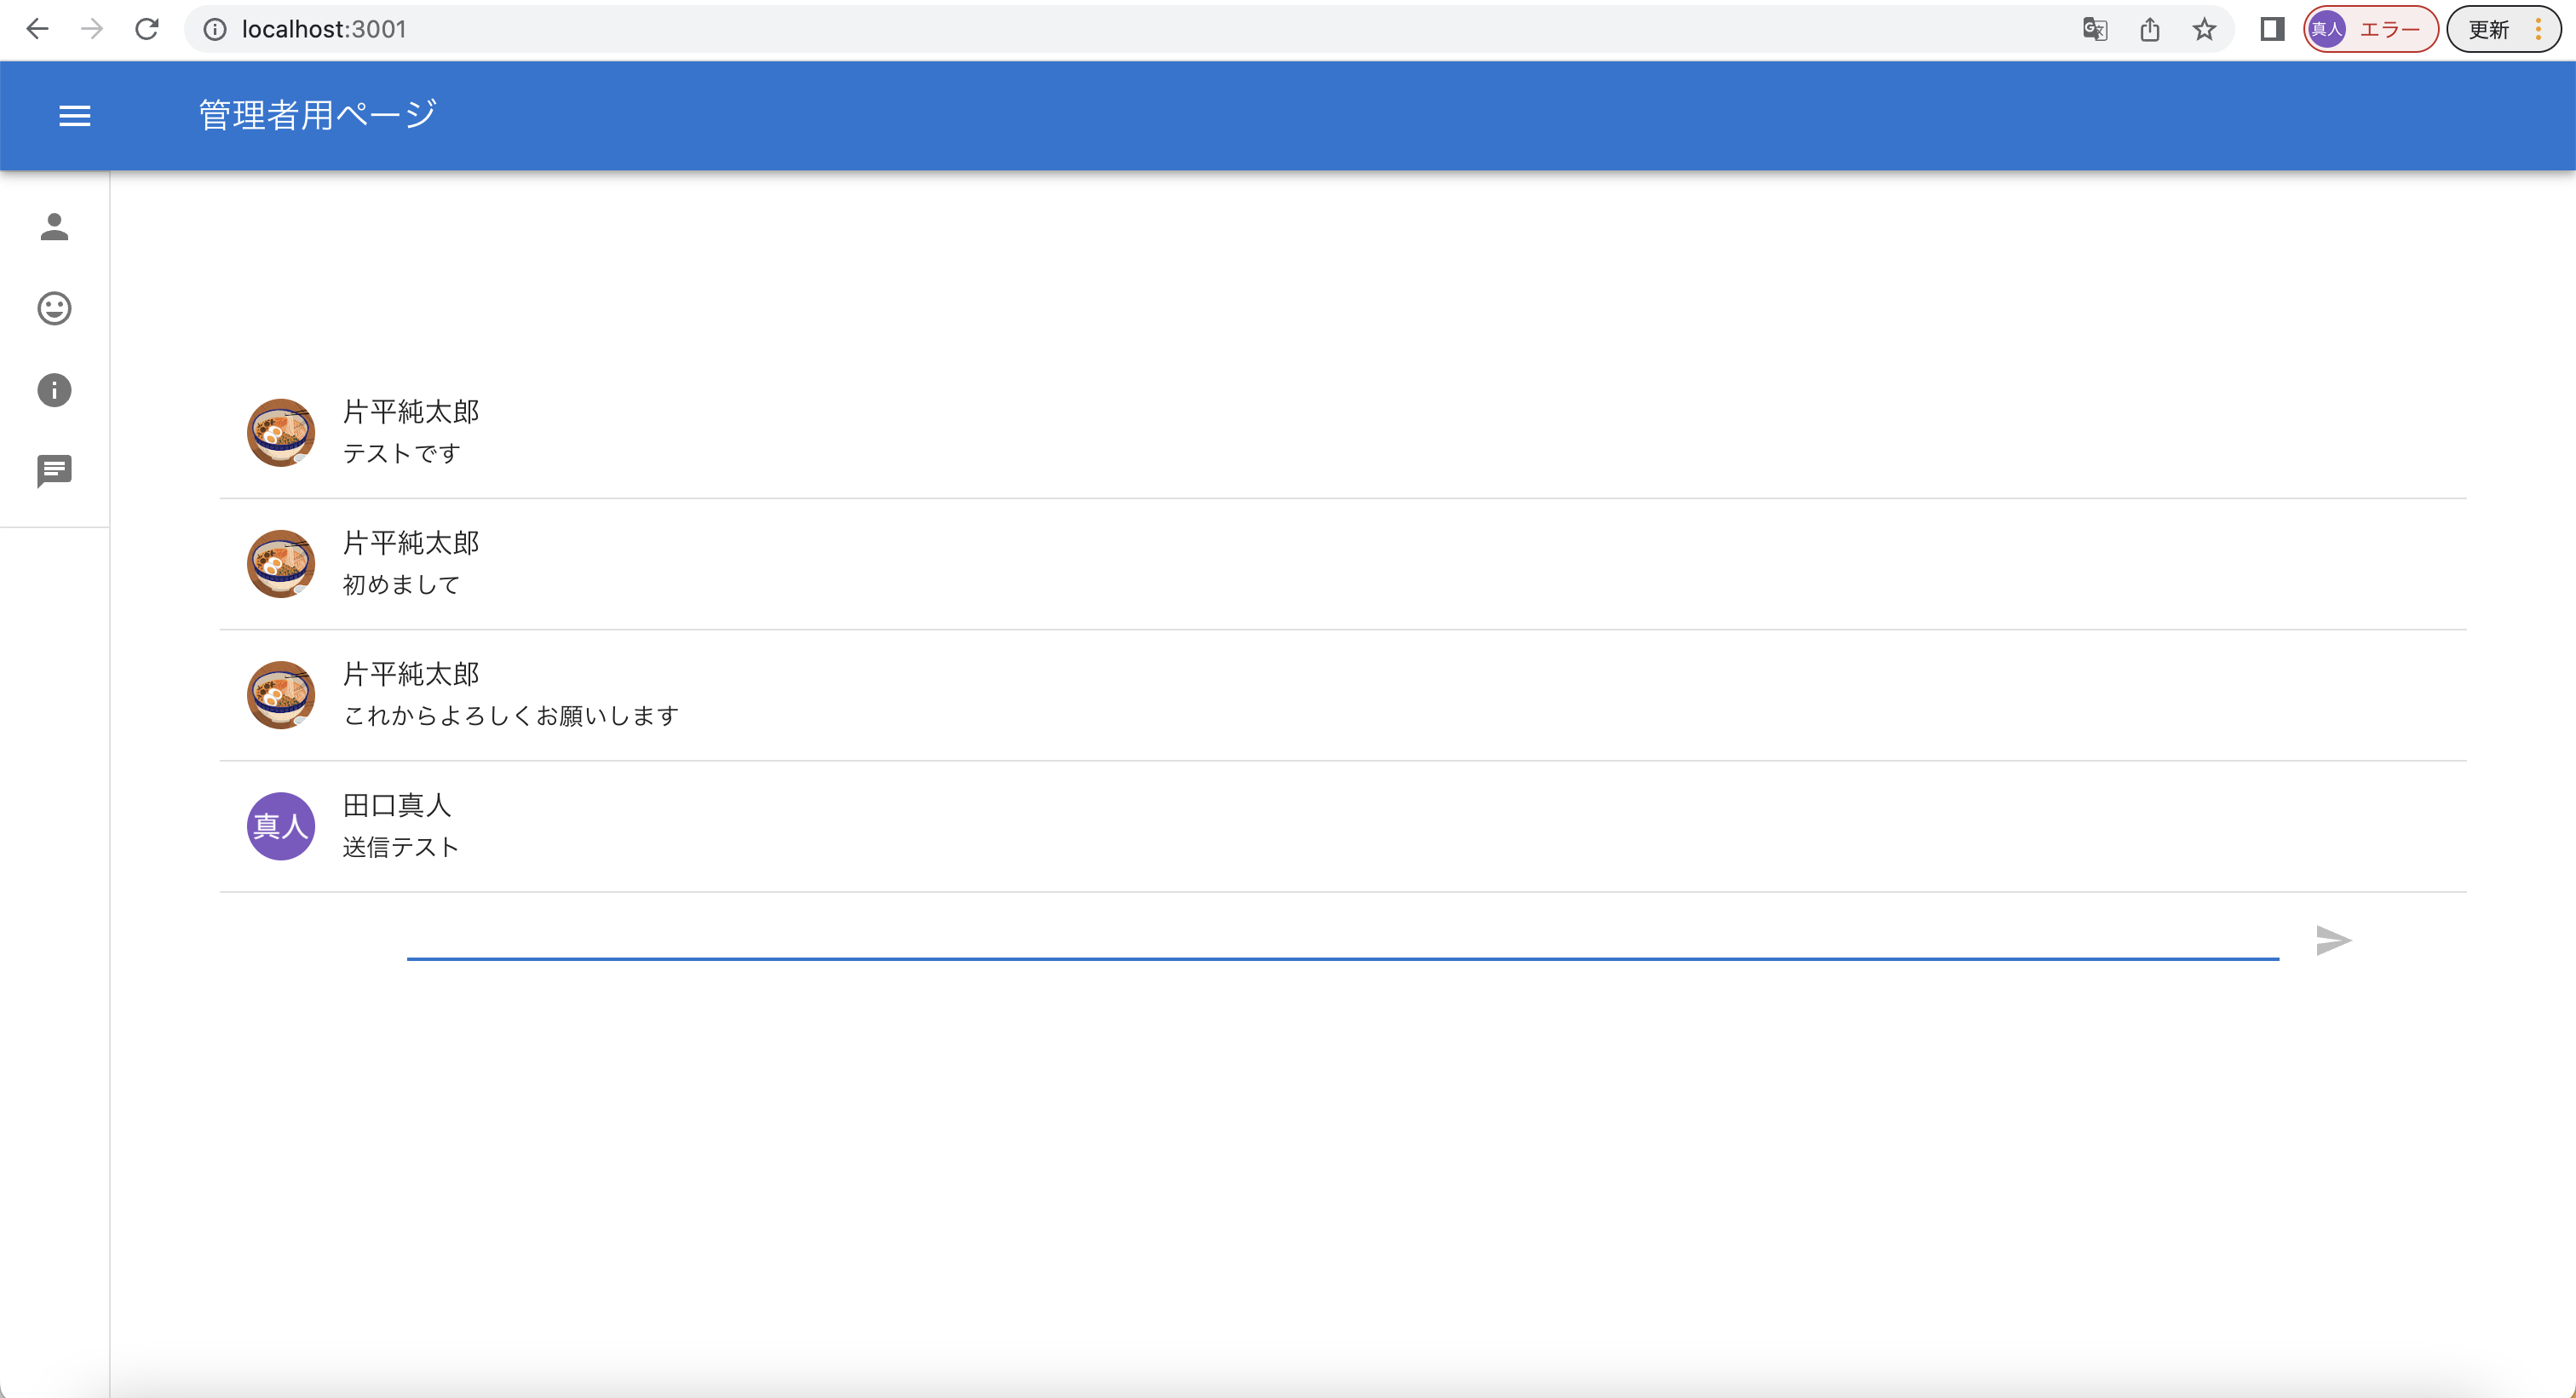
\includegraphics[scale=0.3, clip]{./img/sample16.png}
    \caption{管理者ページから見た掲示板画面}
    \label{fig:図の名前}
  \end{center}
  \end{figure}

  \begin{figure}[!h]
    \begin{center}
      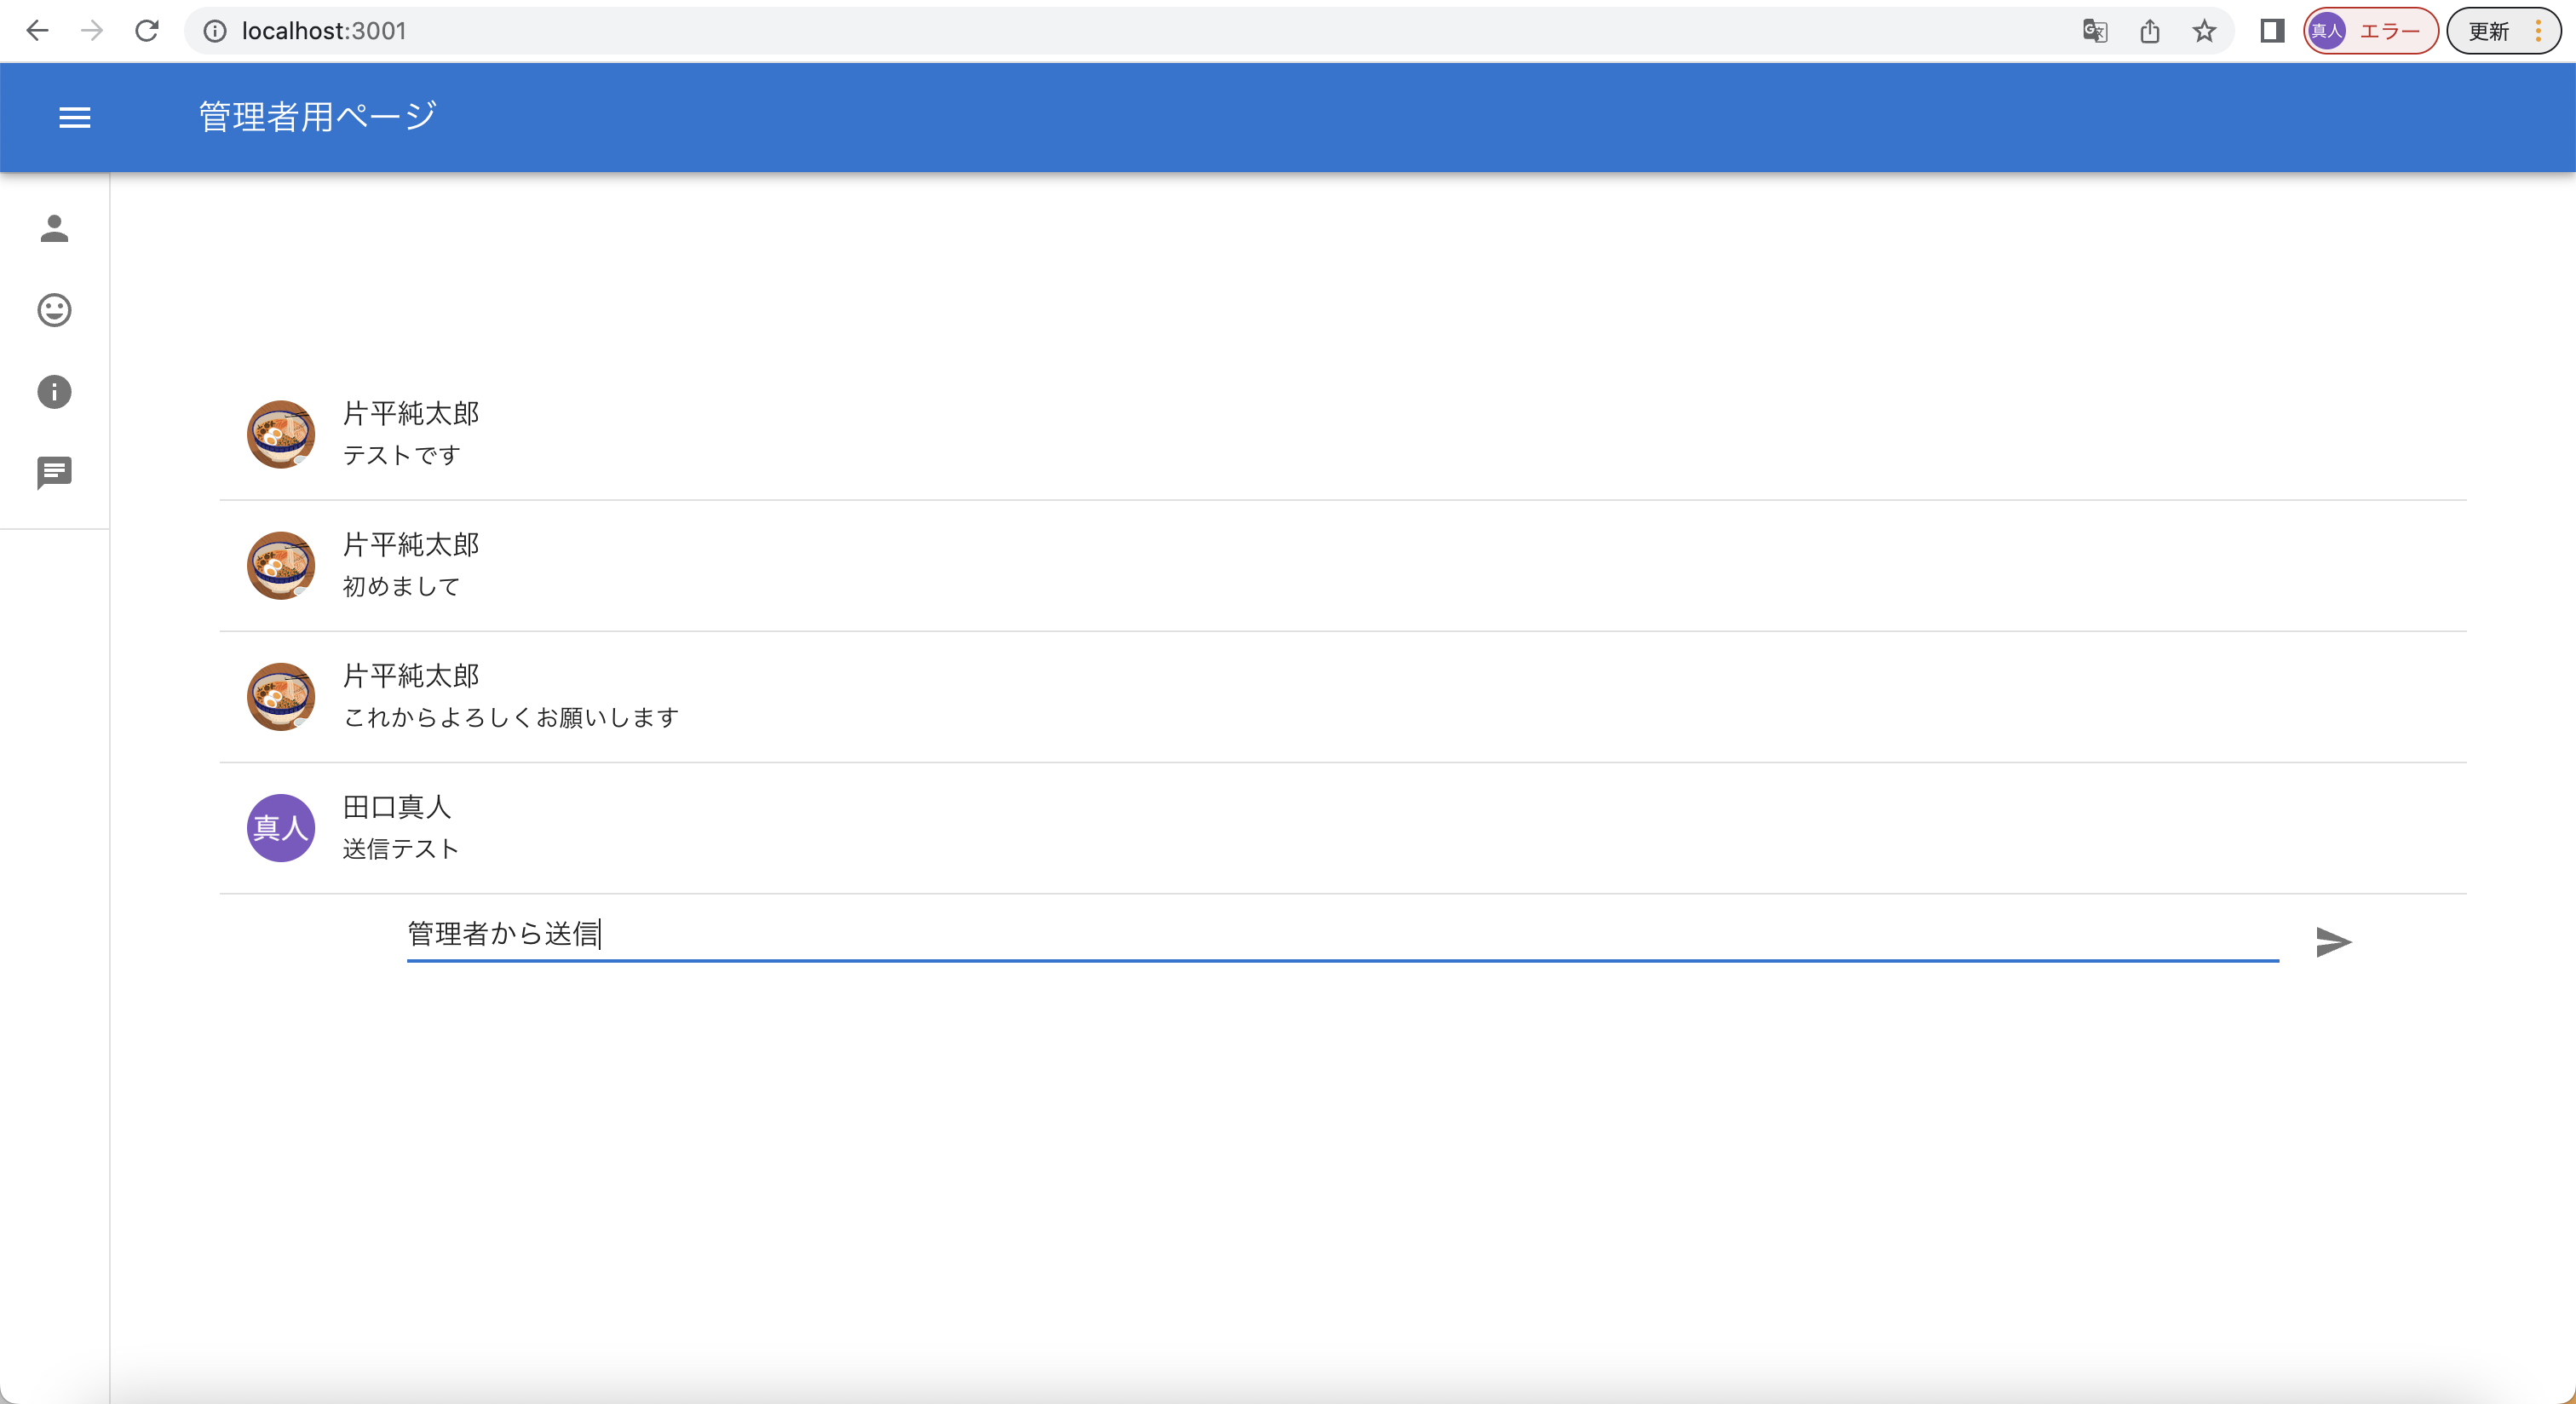
\includegraphics[scale=0.3, clip]{./img/sample17.png}
      \caption{入力画面}
      \label{fig:図の名前}
    \end{center}
    \end{figure}

    \begin{figure}[!h]
      \begin{center}
        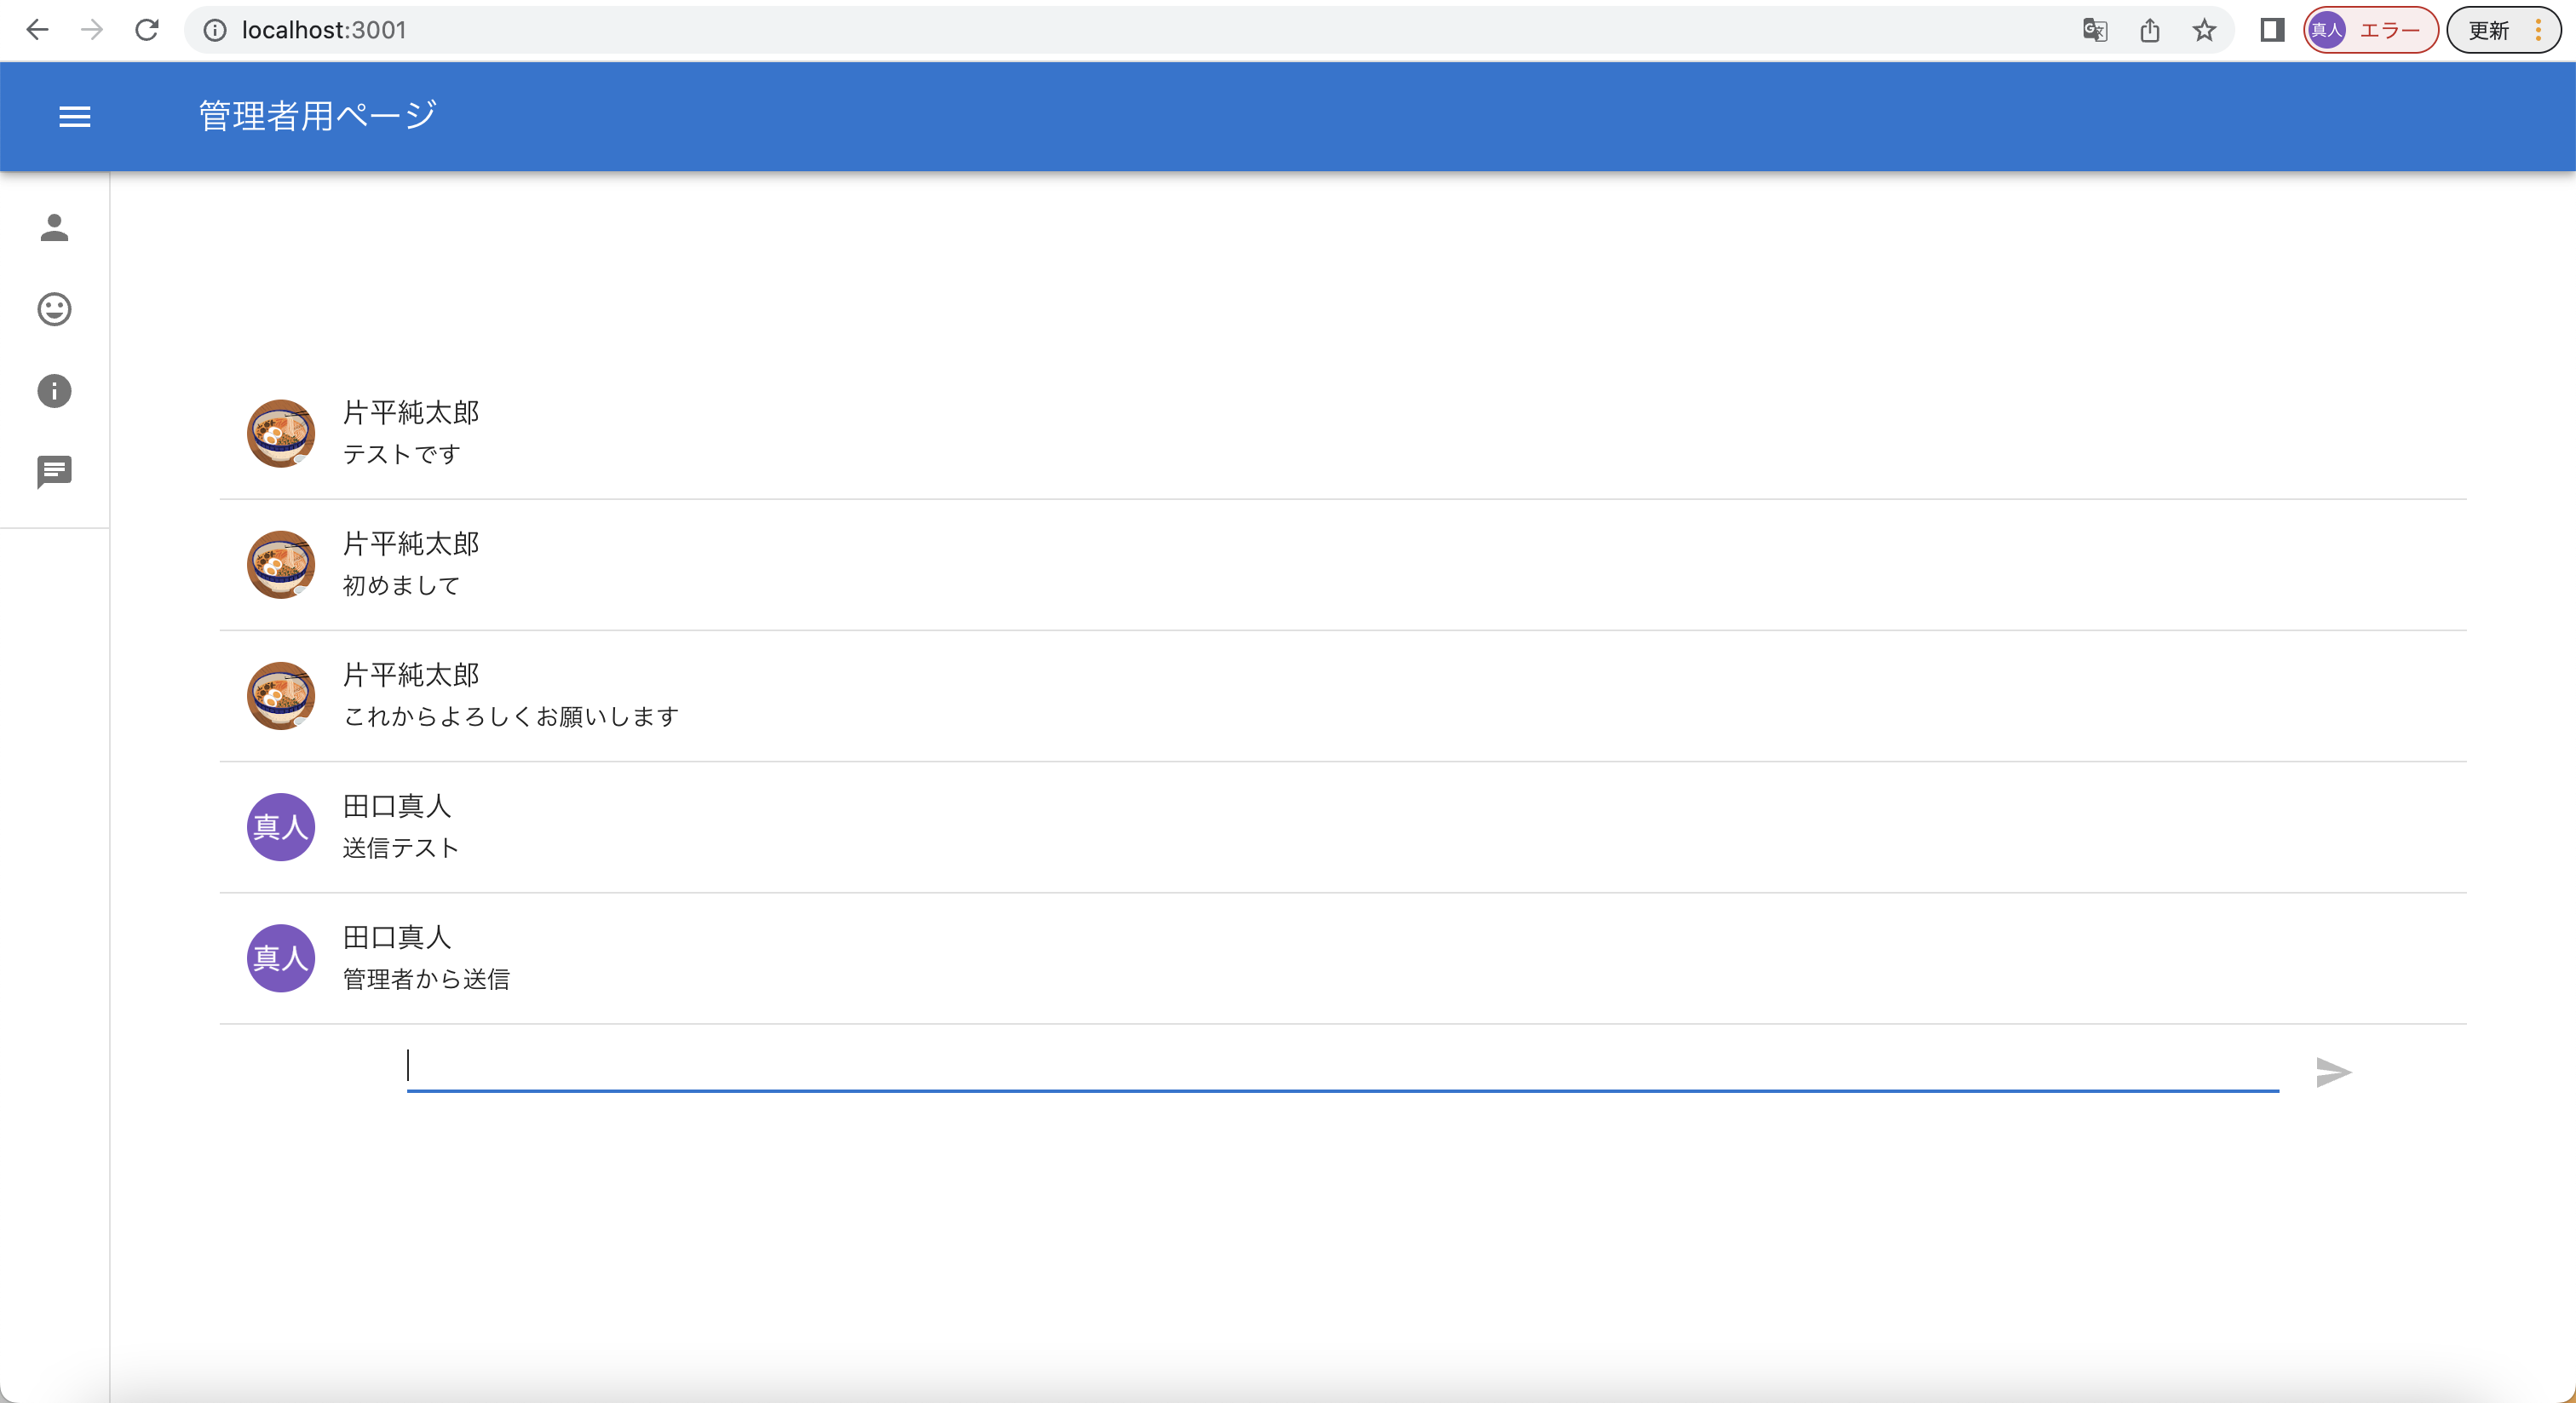
\includegraphics[scale=0.3, clip]{./img/sample18.png}
        \caption{投稿した画面}
        \label{fig:図の名前}
      \end{center}
      \end{figure}

      \begin{figure}[!h]
        \begin{center}
          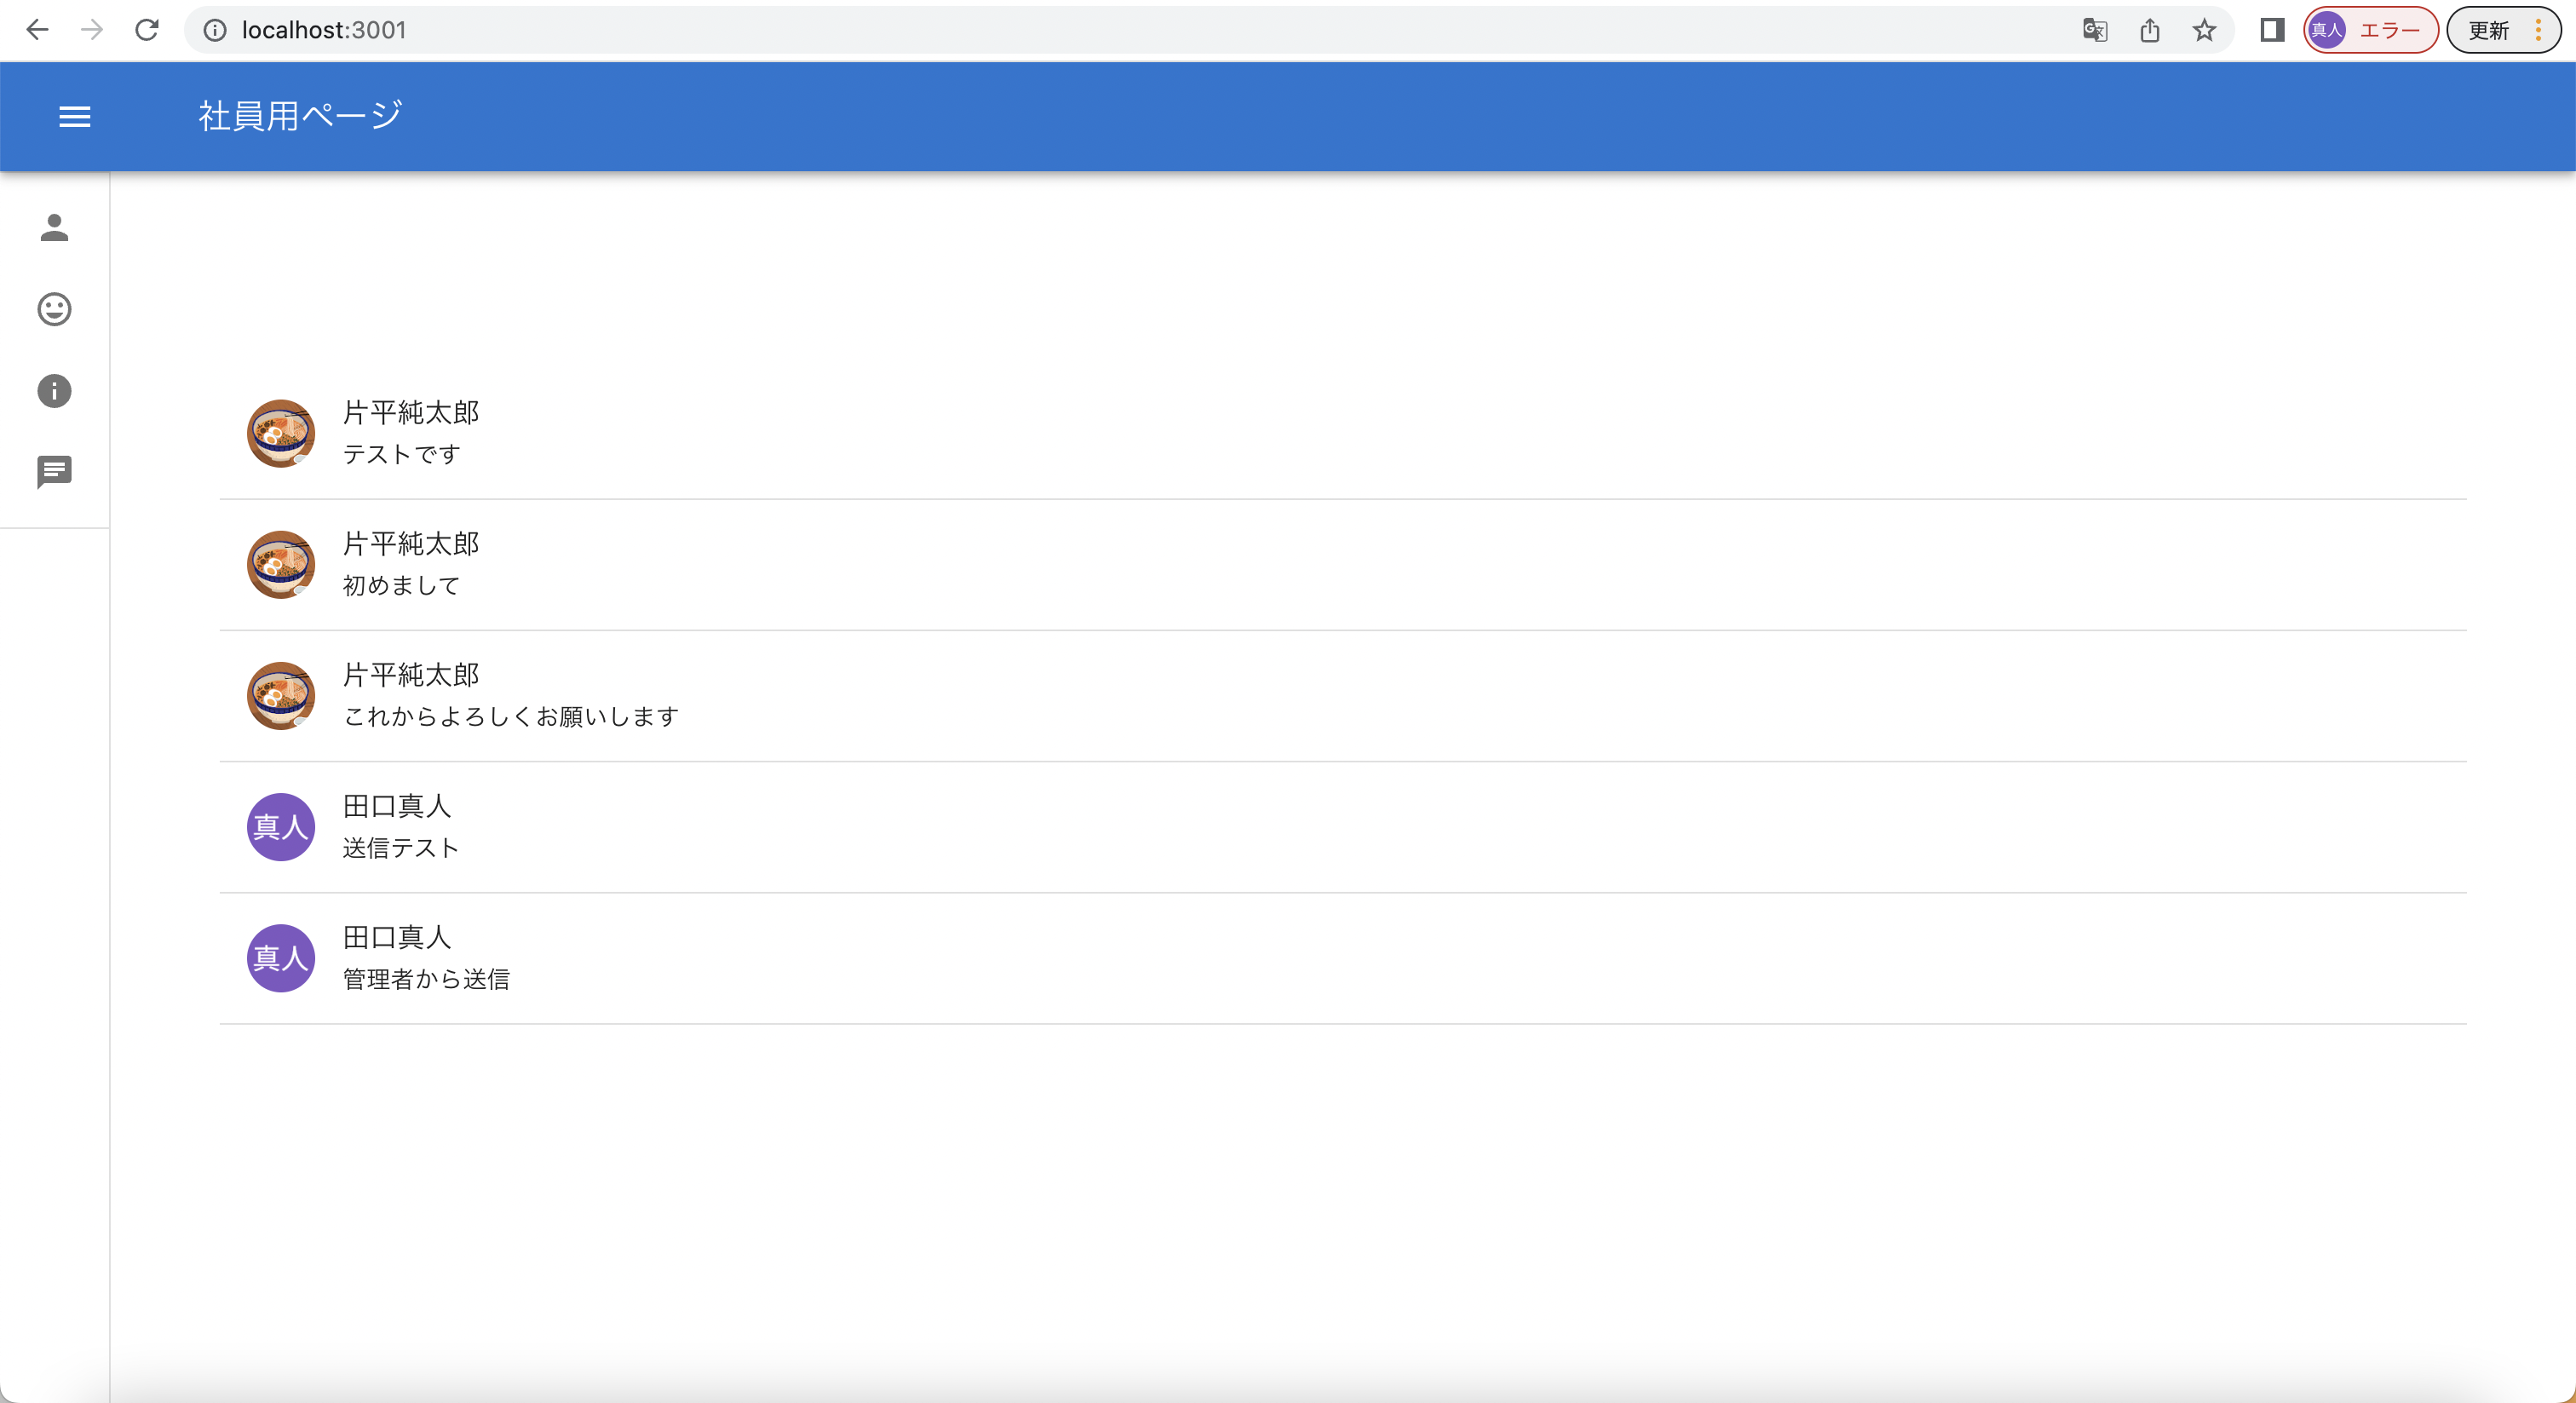
\includegraphics[scale=0.3, clip]{./img/sample19.png}
          \caption{社員ページからの掲示板画面}
          \label{fig:図の名前}
        \end{center}
        \end{figure}

\clearpage

\section{チャット機能}
管理者が社員一人一人にコミュニケーションを取るための機能である.
管理者のみがルームを作成でき,管理者,社員どちらからもメッセージのやり取りができる. \\
図4.20のトークボタンから社員のチャットルームを作成できる.図4.21はトークボタンを押した後の
画面である.図4.22,図4.23はメッセージを入力して,送信した画面である.図4.24は作成されたトークルーム一覧のページである.
図4.25,図4.26は社員用ページのトーク画面である.
管理者が送信した「こんにちは」というメッセージが社員用ページでも見れることが確認できた.
図4.27,図4.28は社員から管理者に向けてメッセージを送信した画面である.
図4.29は管理者から見た社員とのトーク画面である.社員が送信した「こんにちは」
というメッセージが管理者用ページでも見れることが確認できた.


\vspace{15mm}

\begin{figure}[!h]
  \begin{center}
    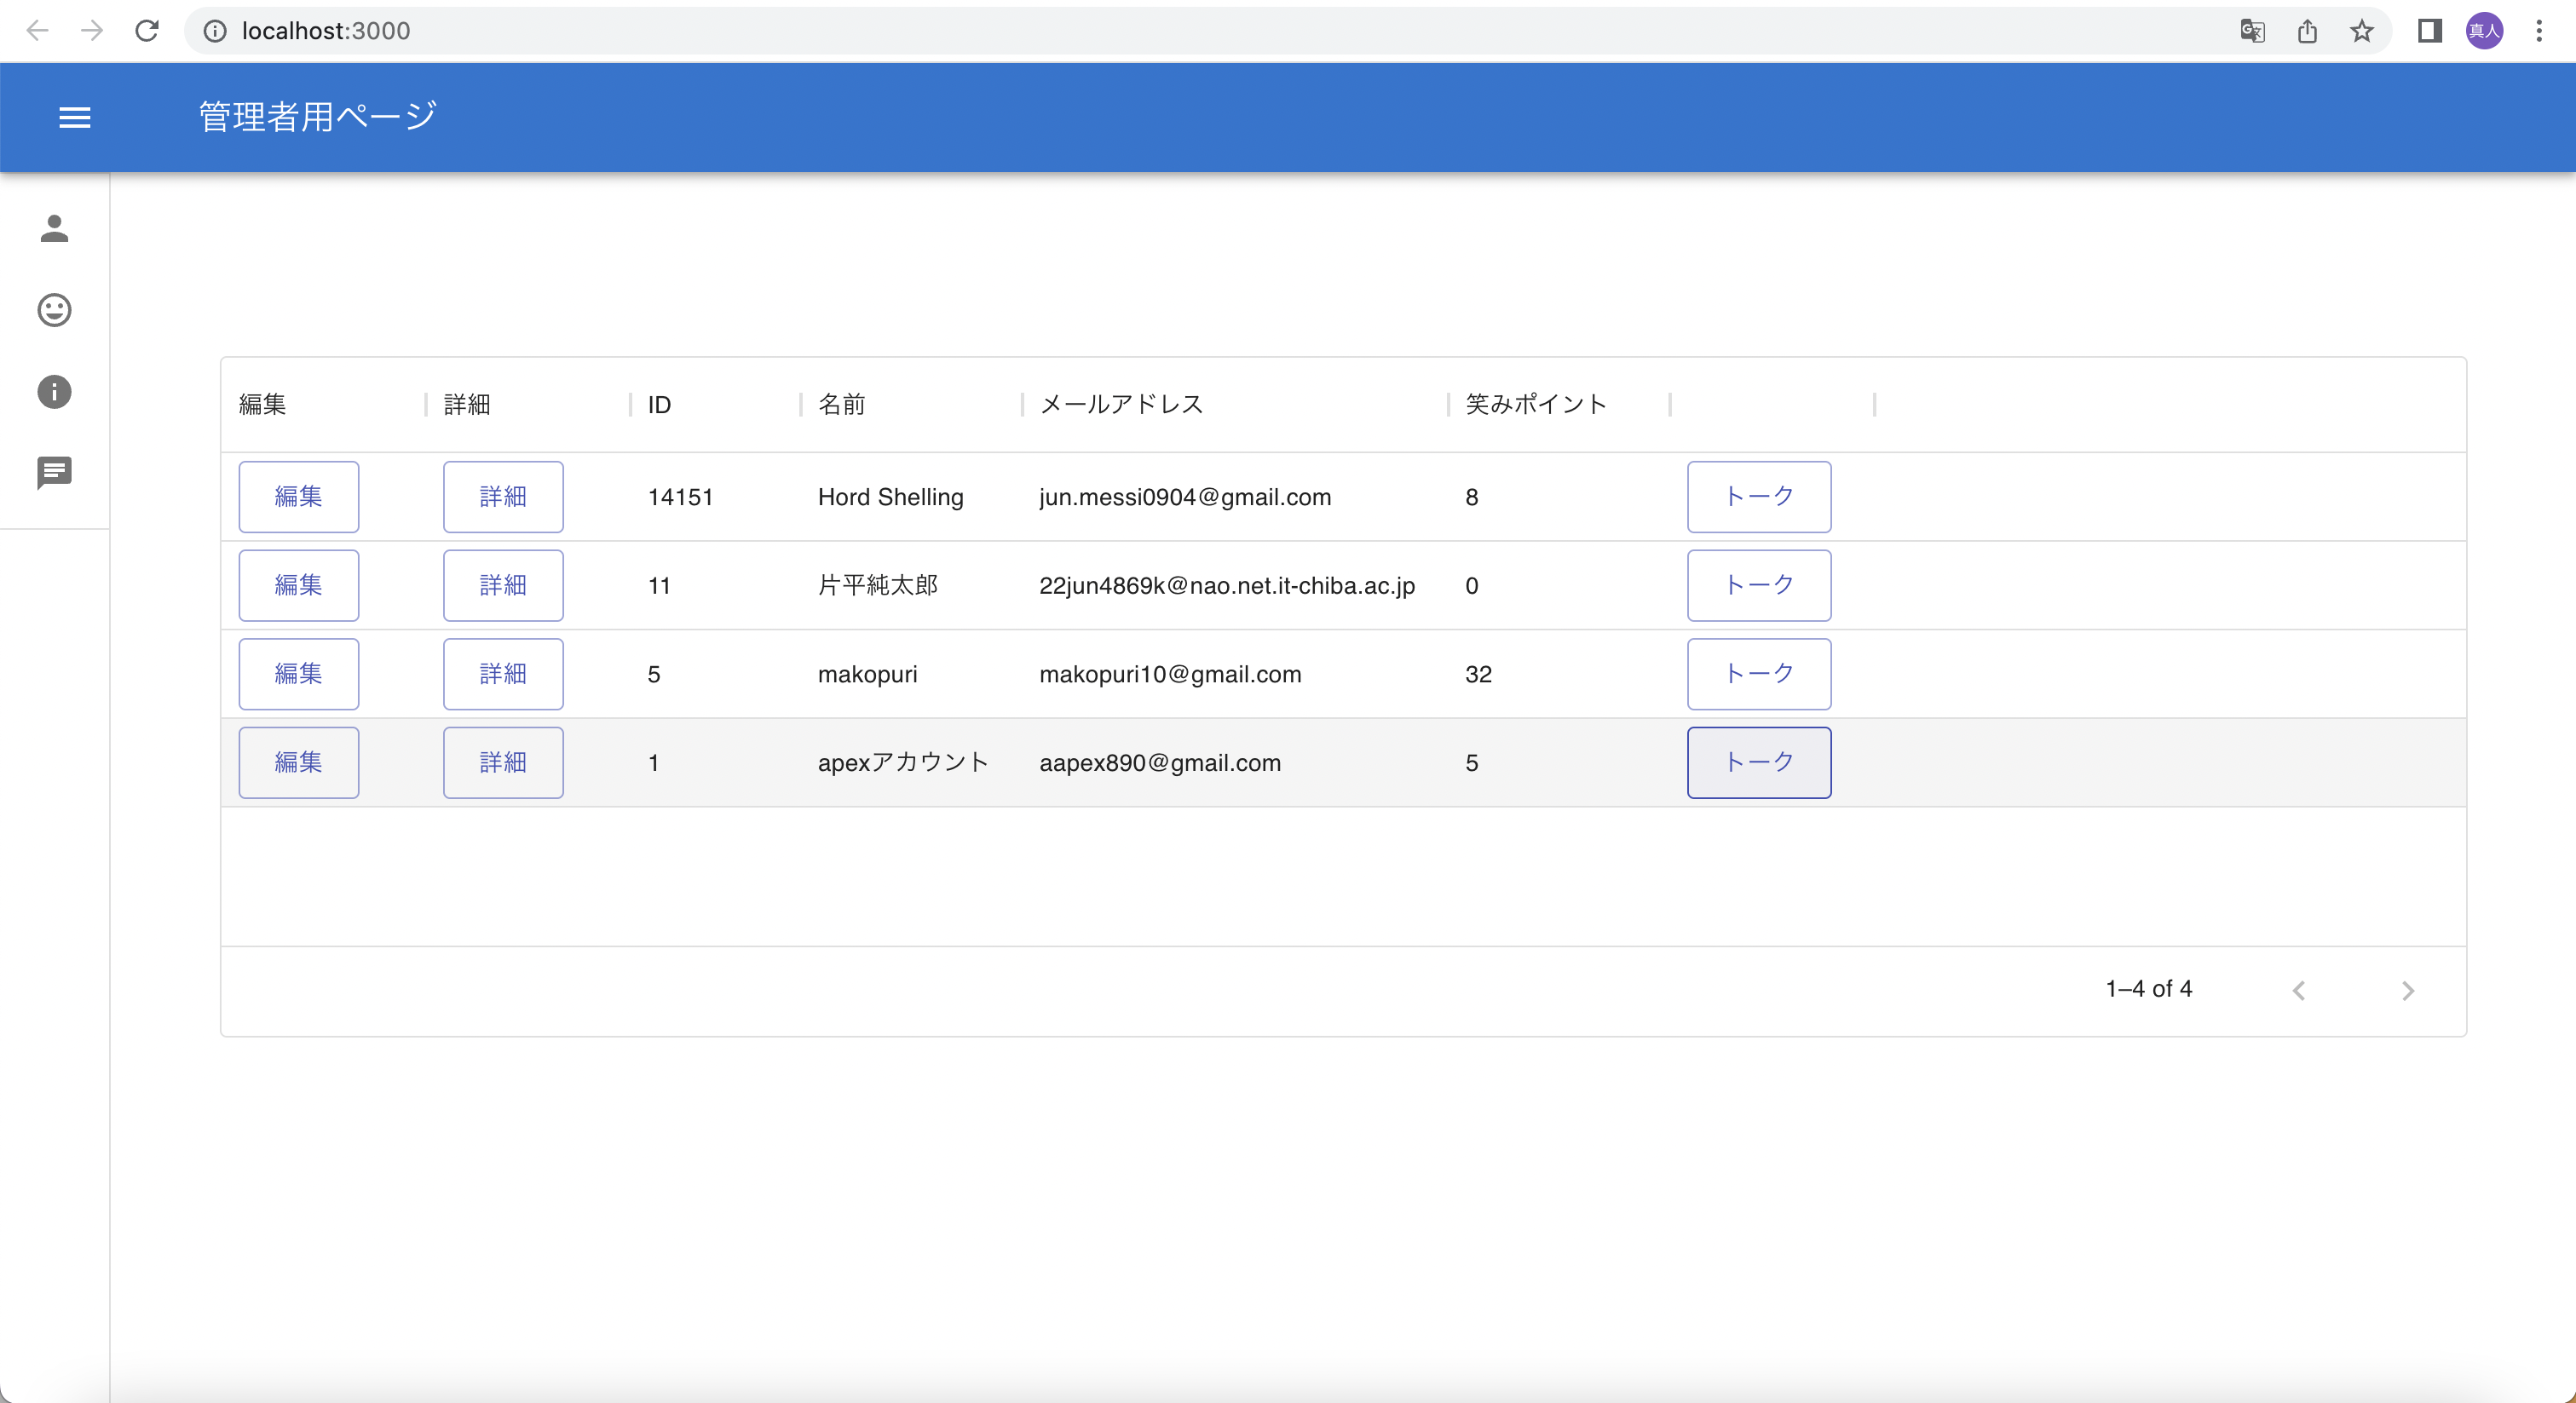
\includegraphics[scale=0.3, clip]{./img/chat1.png}
    \caption{管理者画面}
    \label{fig:図の名前}
  \end{center}
  \end{figure}

  \begin{figure}[!h]
    \begin{center}
      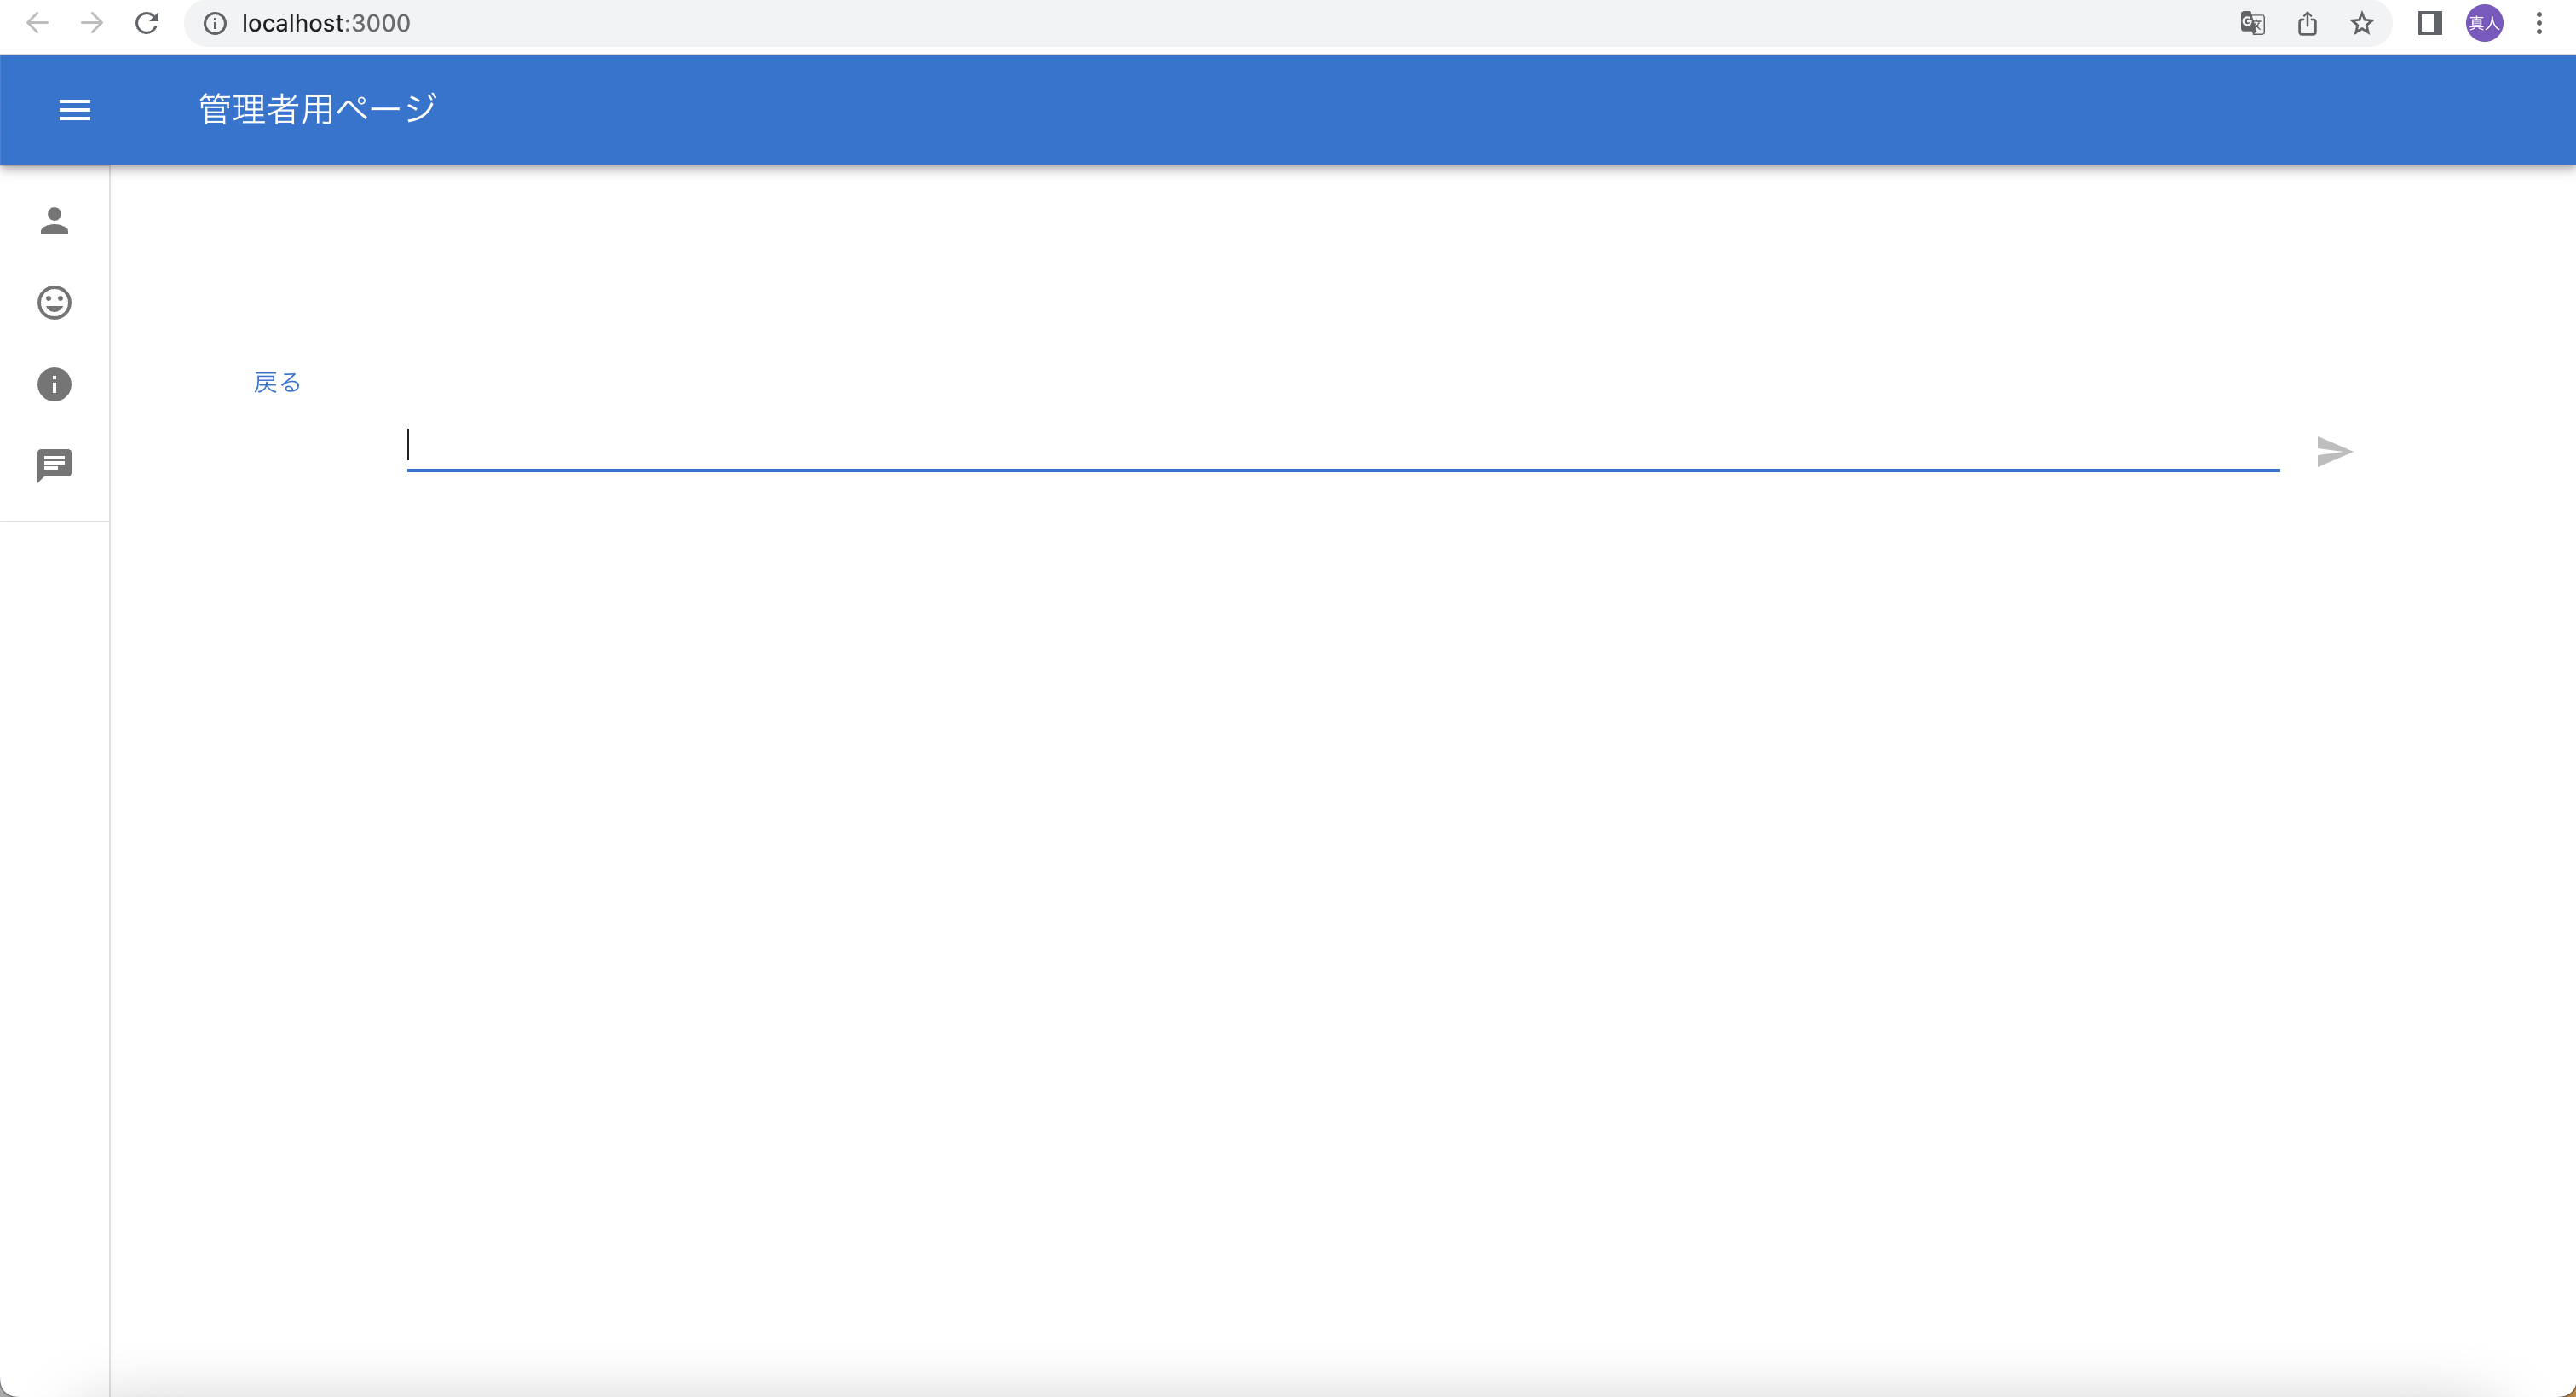
\includegraphics[scale=0.3, clip]{./img/chat2.png}
      \caption{トークボタン押した後の画面}
      \label{fig:図の名前}
    \end{center}
    \end{figure}

    \begin{figure}[!h]
      \begin{center}
        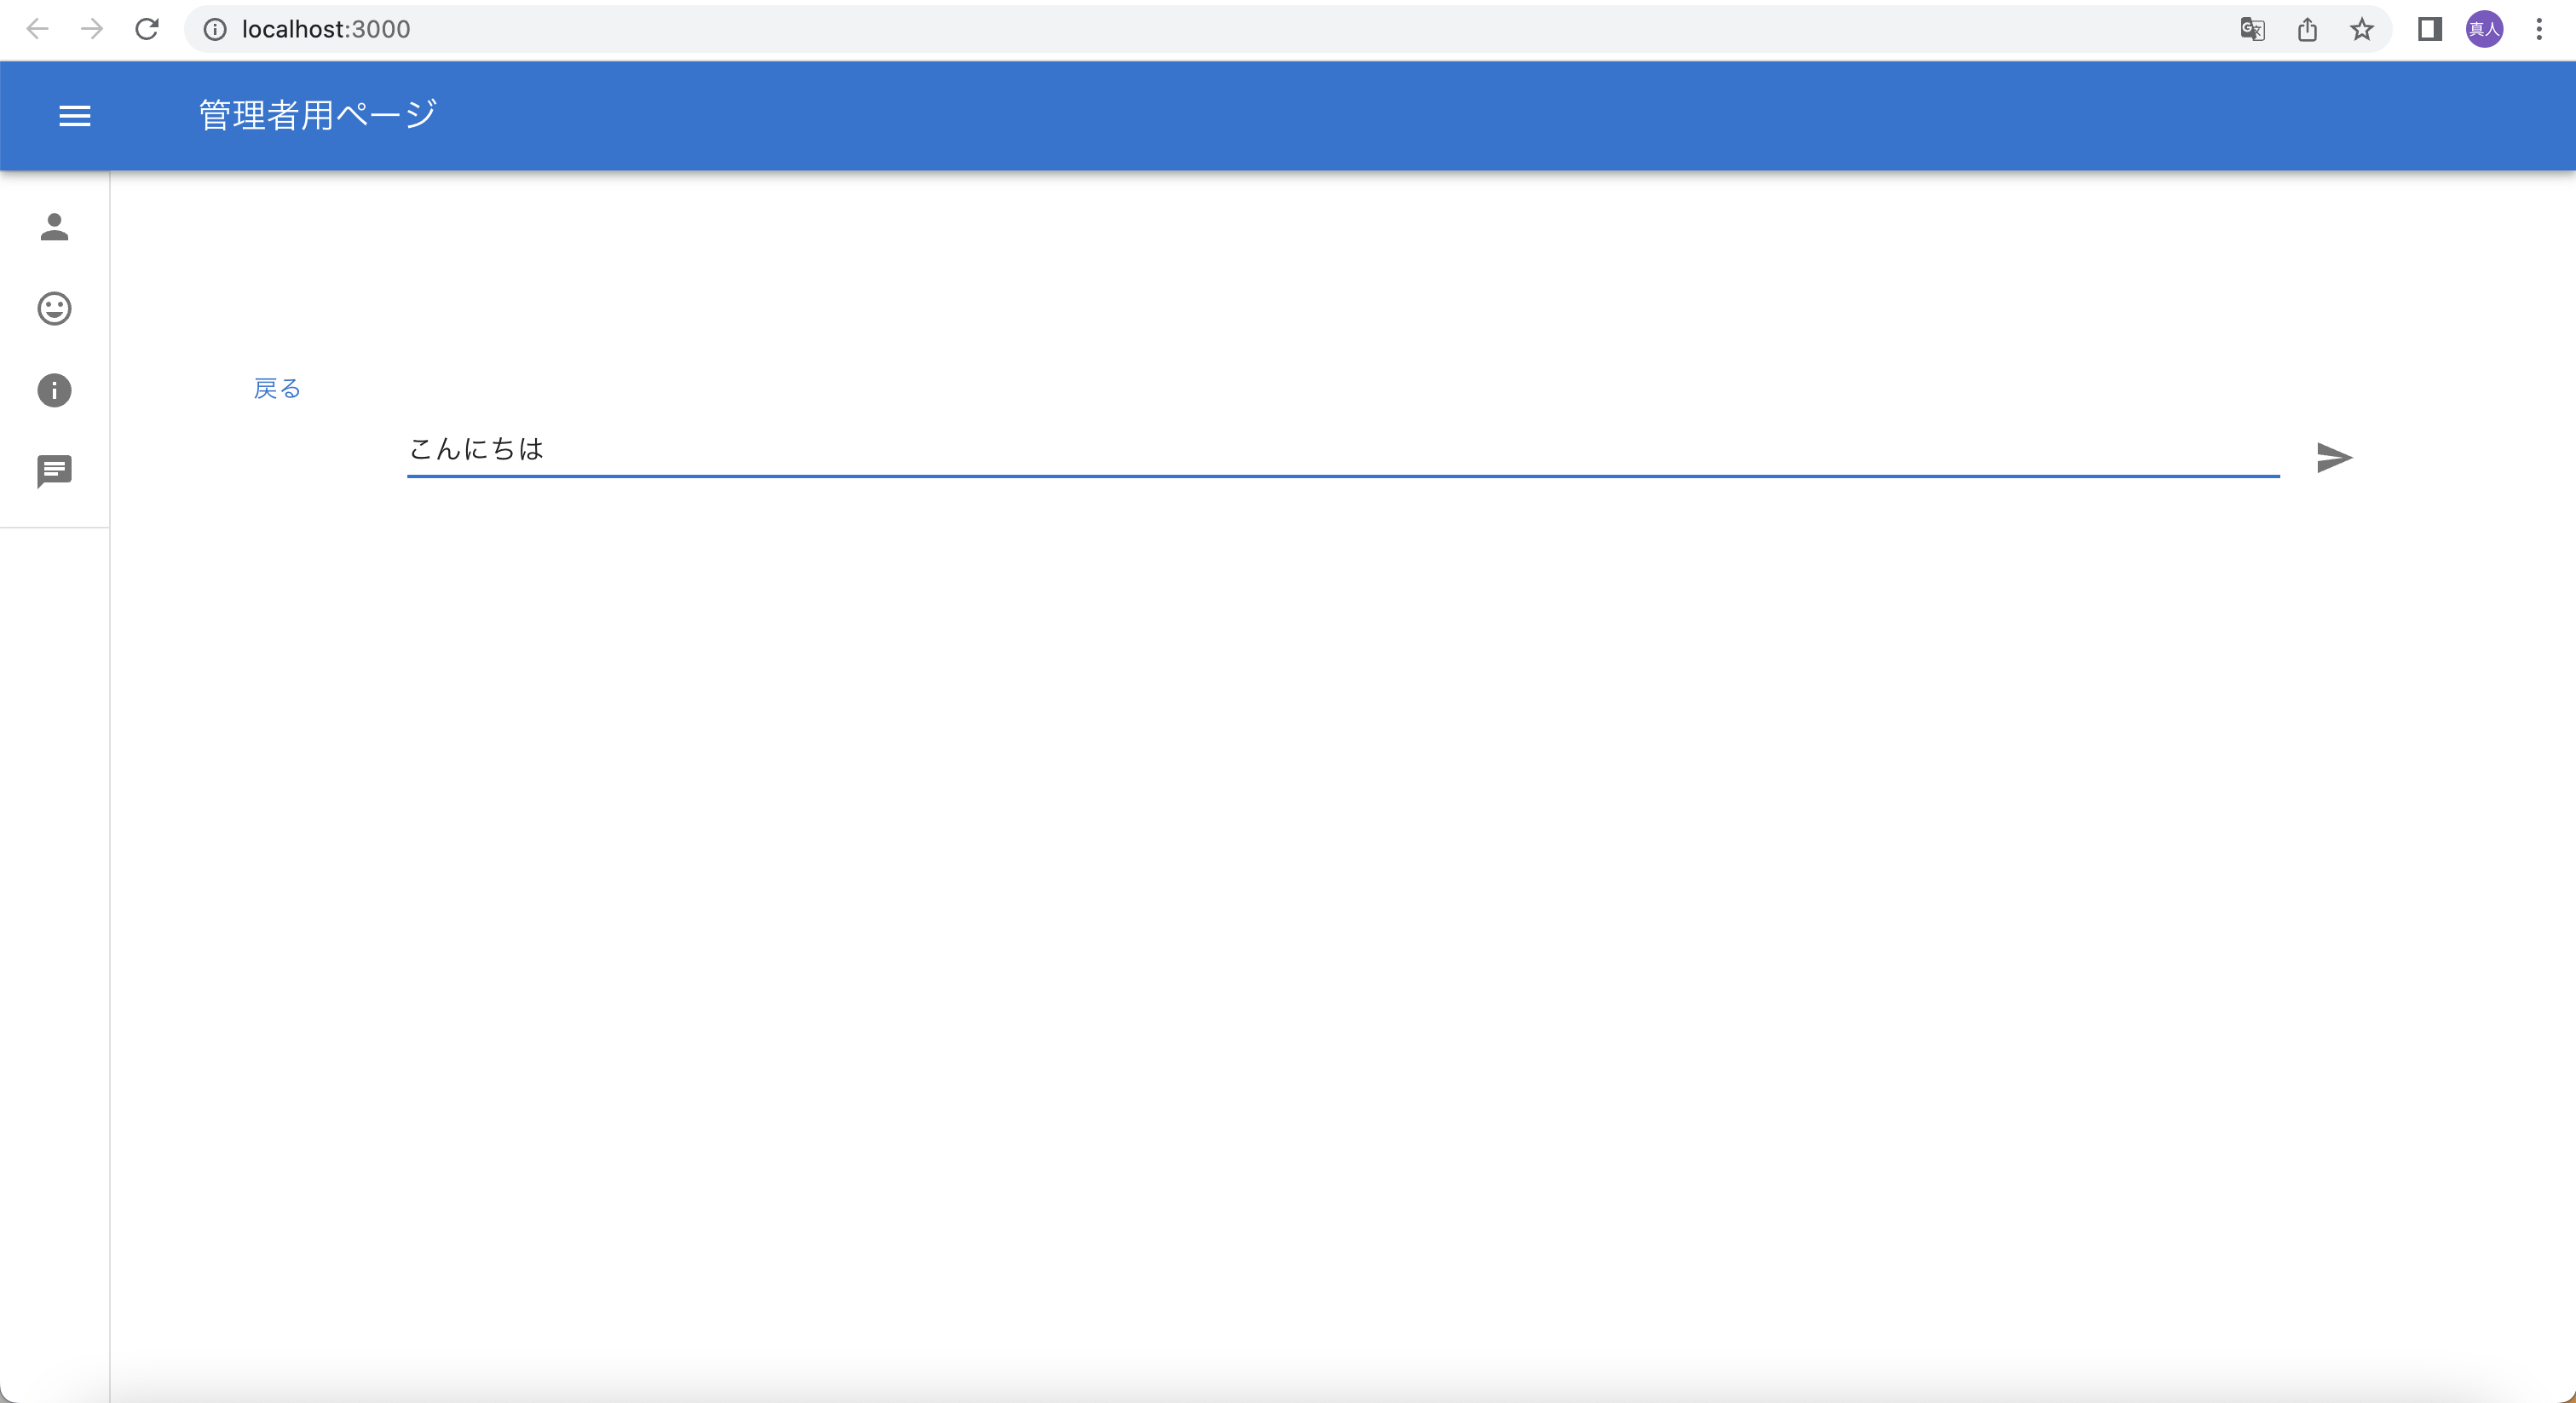
\includegraphics[scale=0.3, clip]{./img/chat3.png}
        \caption{メッセージ入力画面}
        \label{fig:図の名前}
      \end{center}
      \end{figure}

      \begin{figure}[!h]
        \begin{center}
          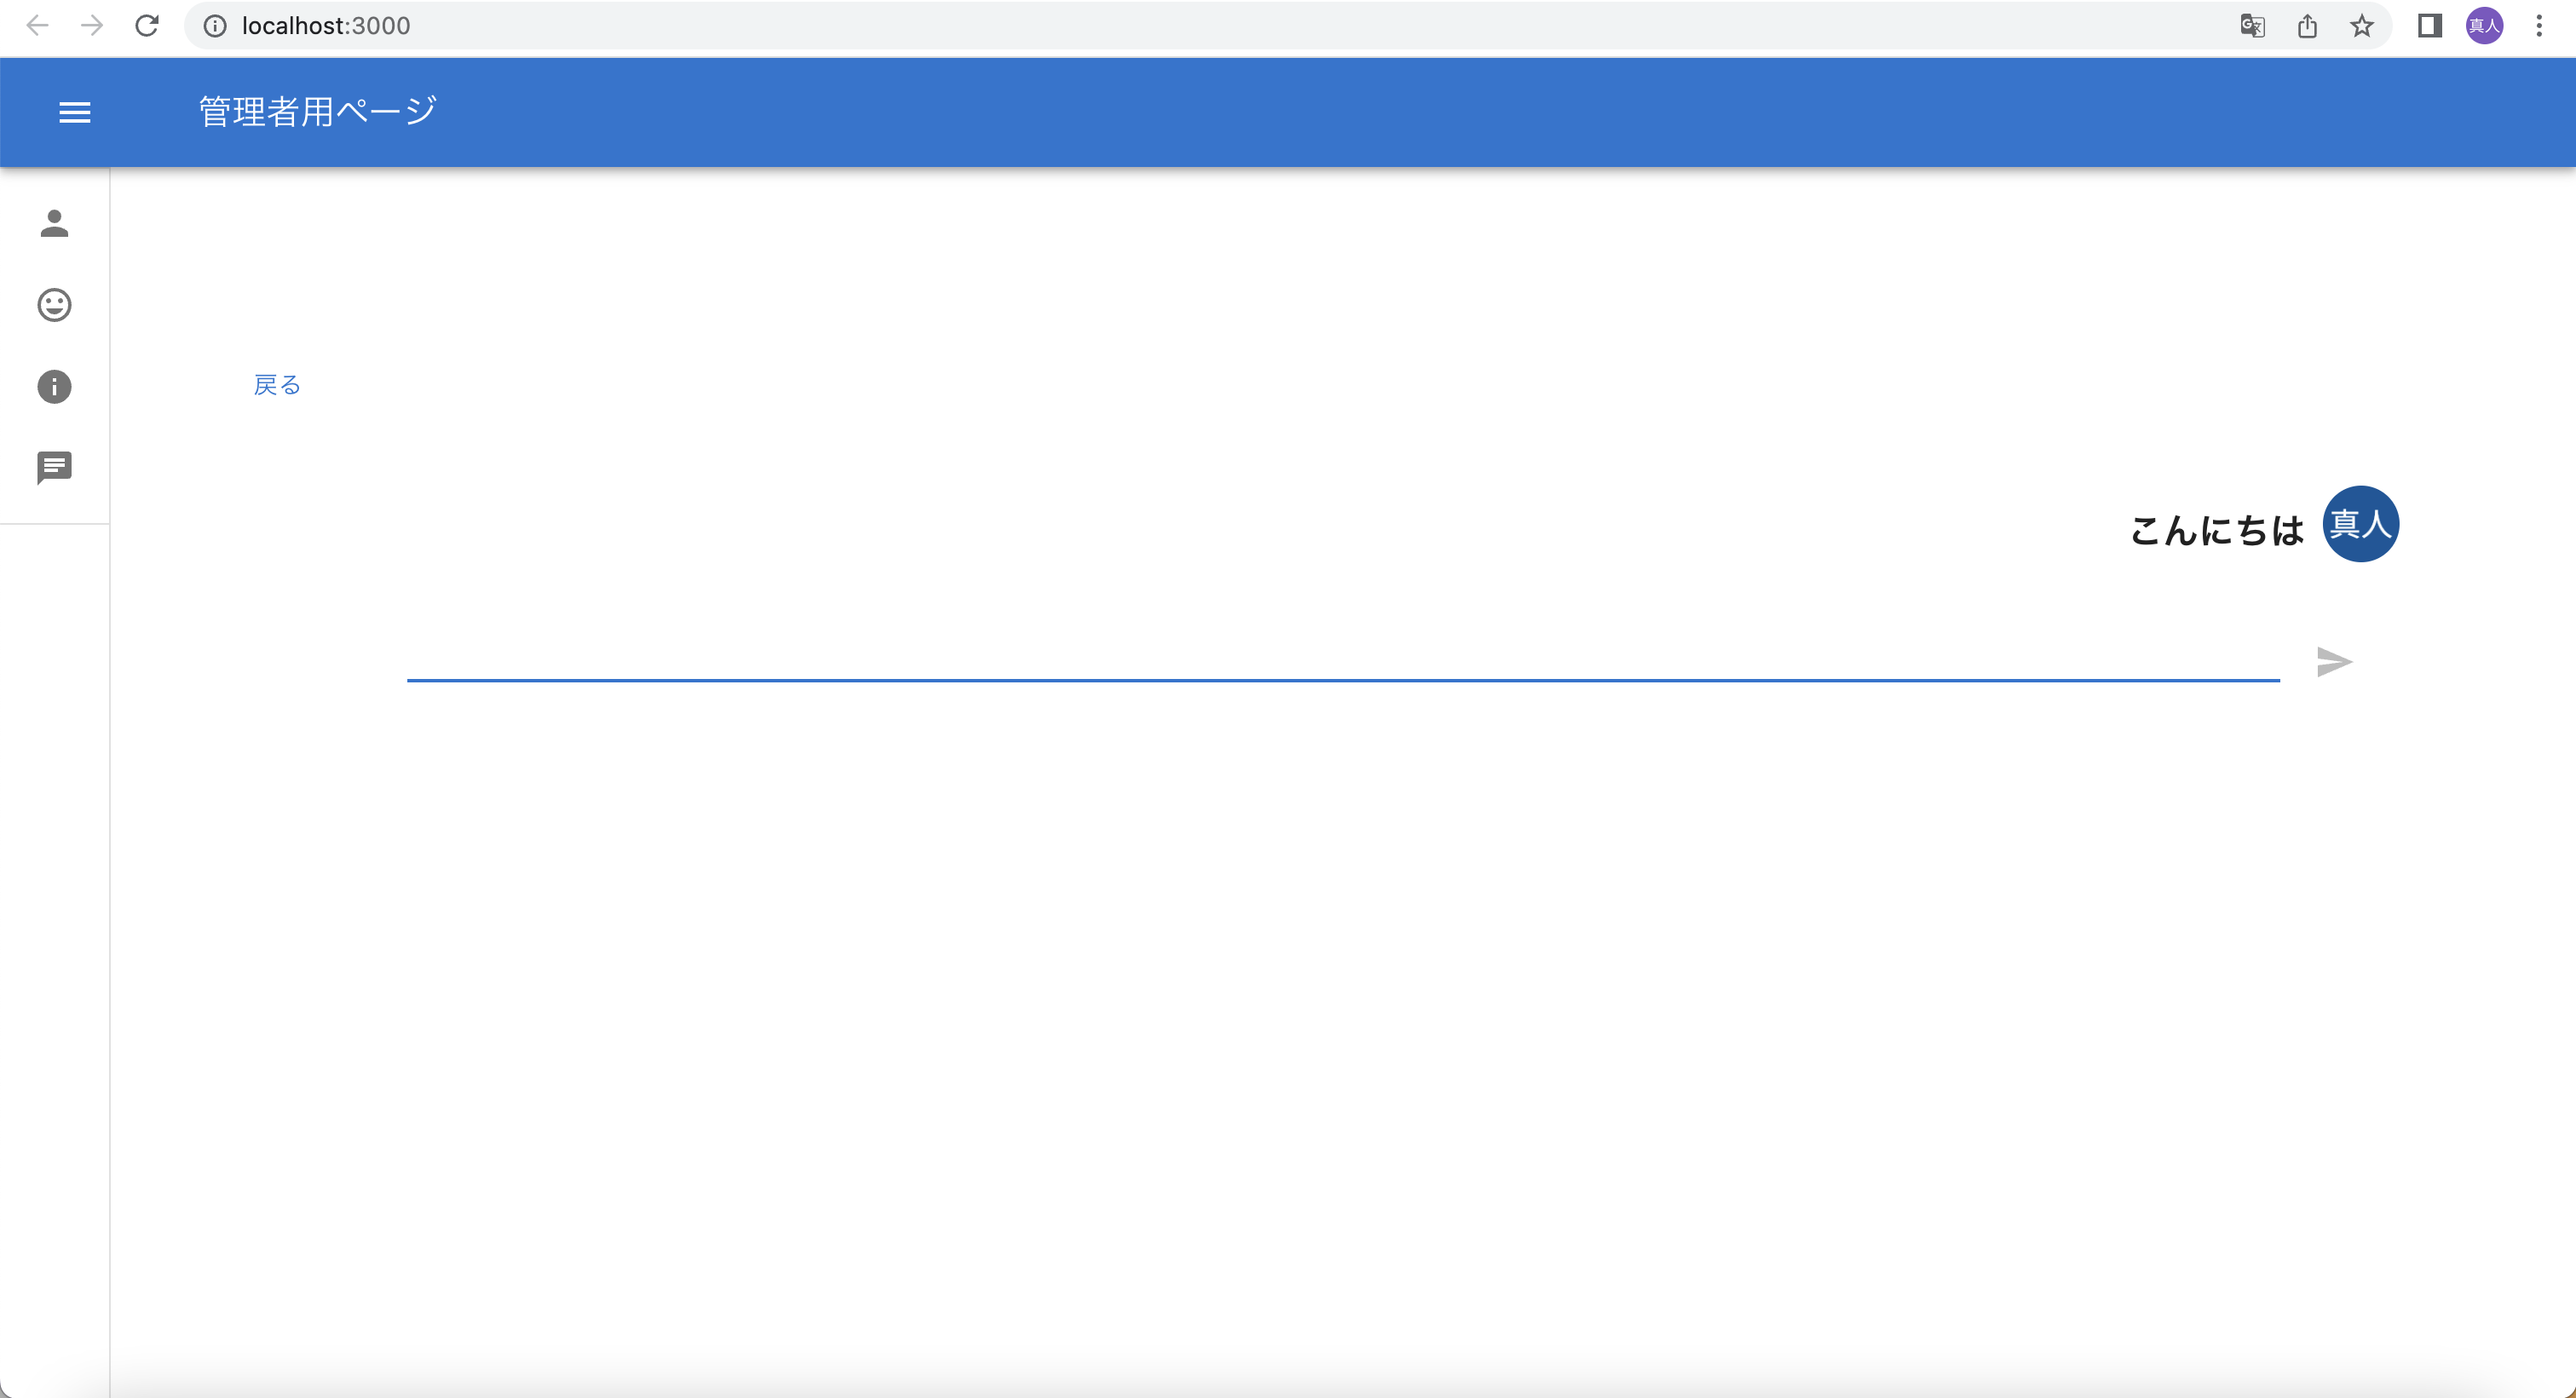
\includegraphics[scale=0.3, clip]{./img/chat4.png}
          \caption{送信した後の画面}
          \label{fig:図の名前}
        \end{center}
        \end{figure}

        \begin{figure}[!h]
          \begin{center}
            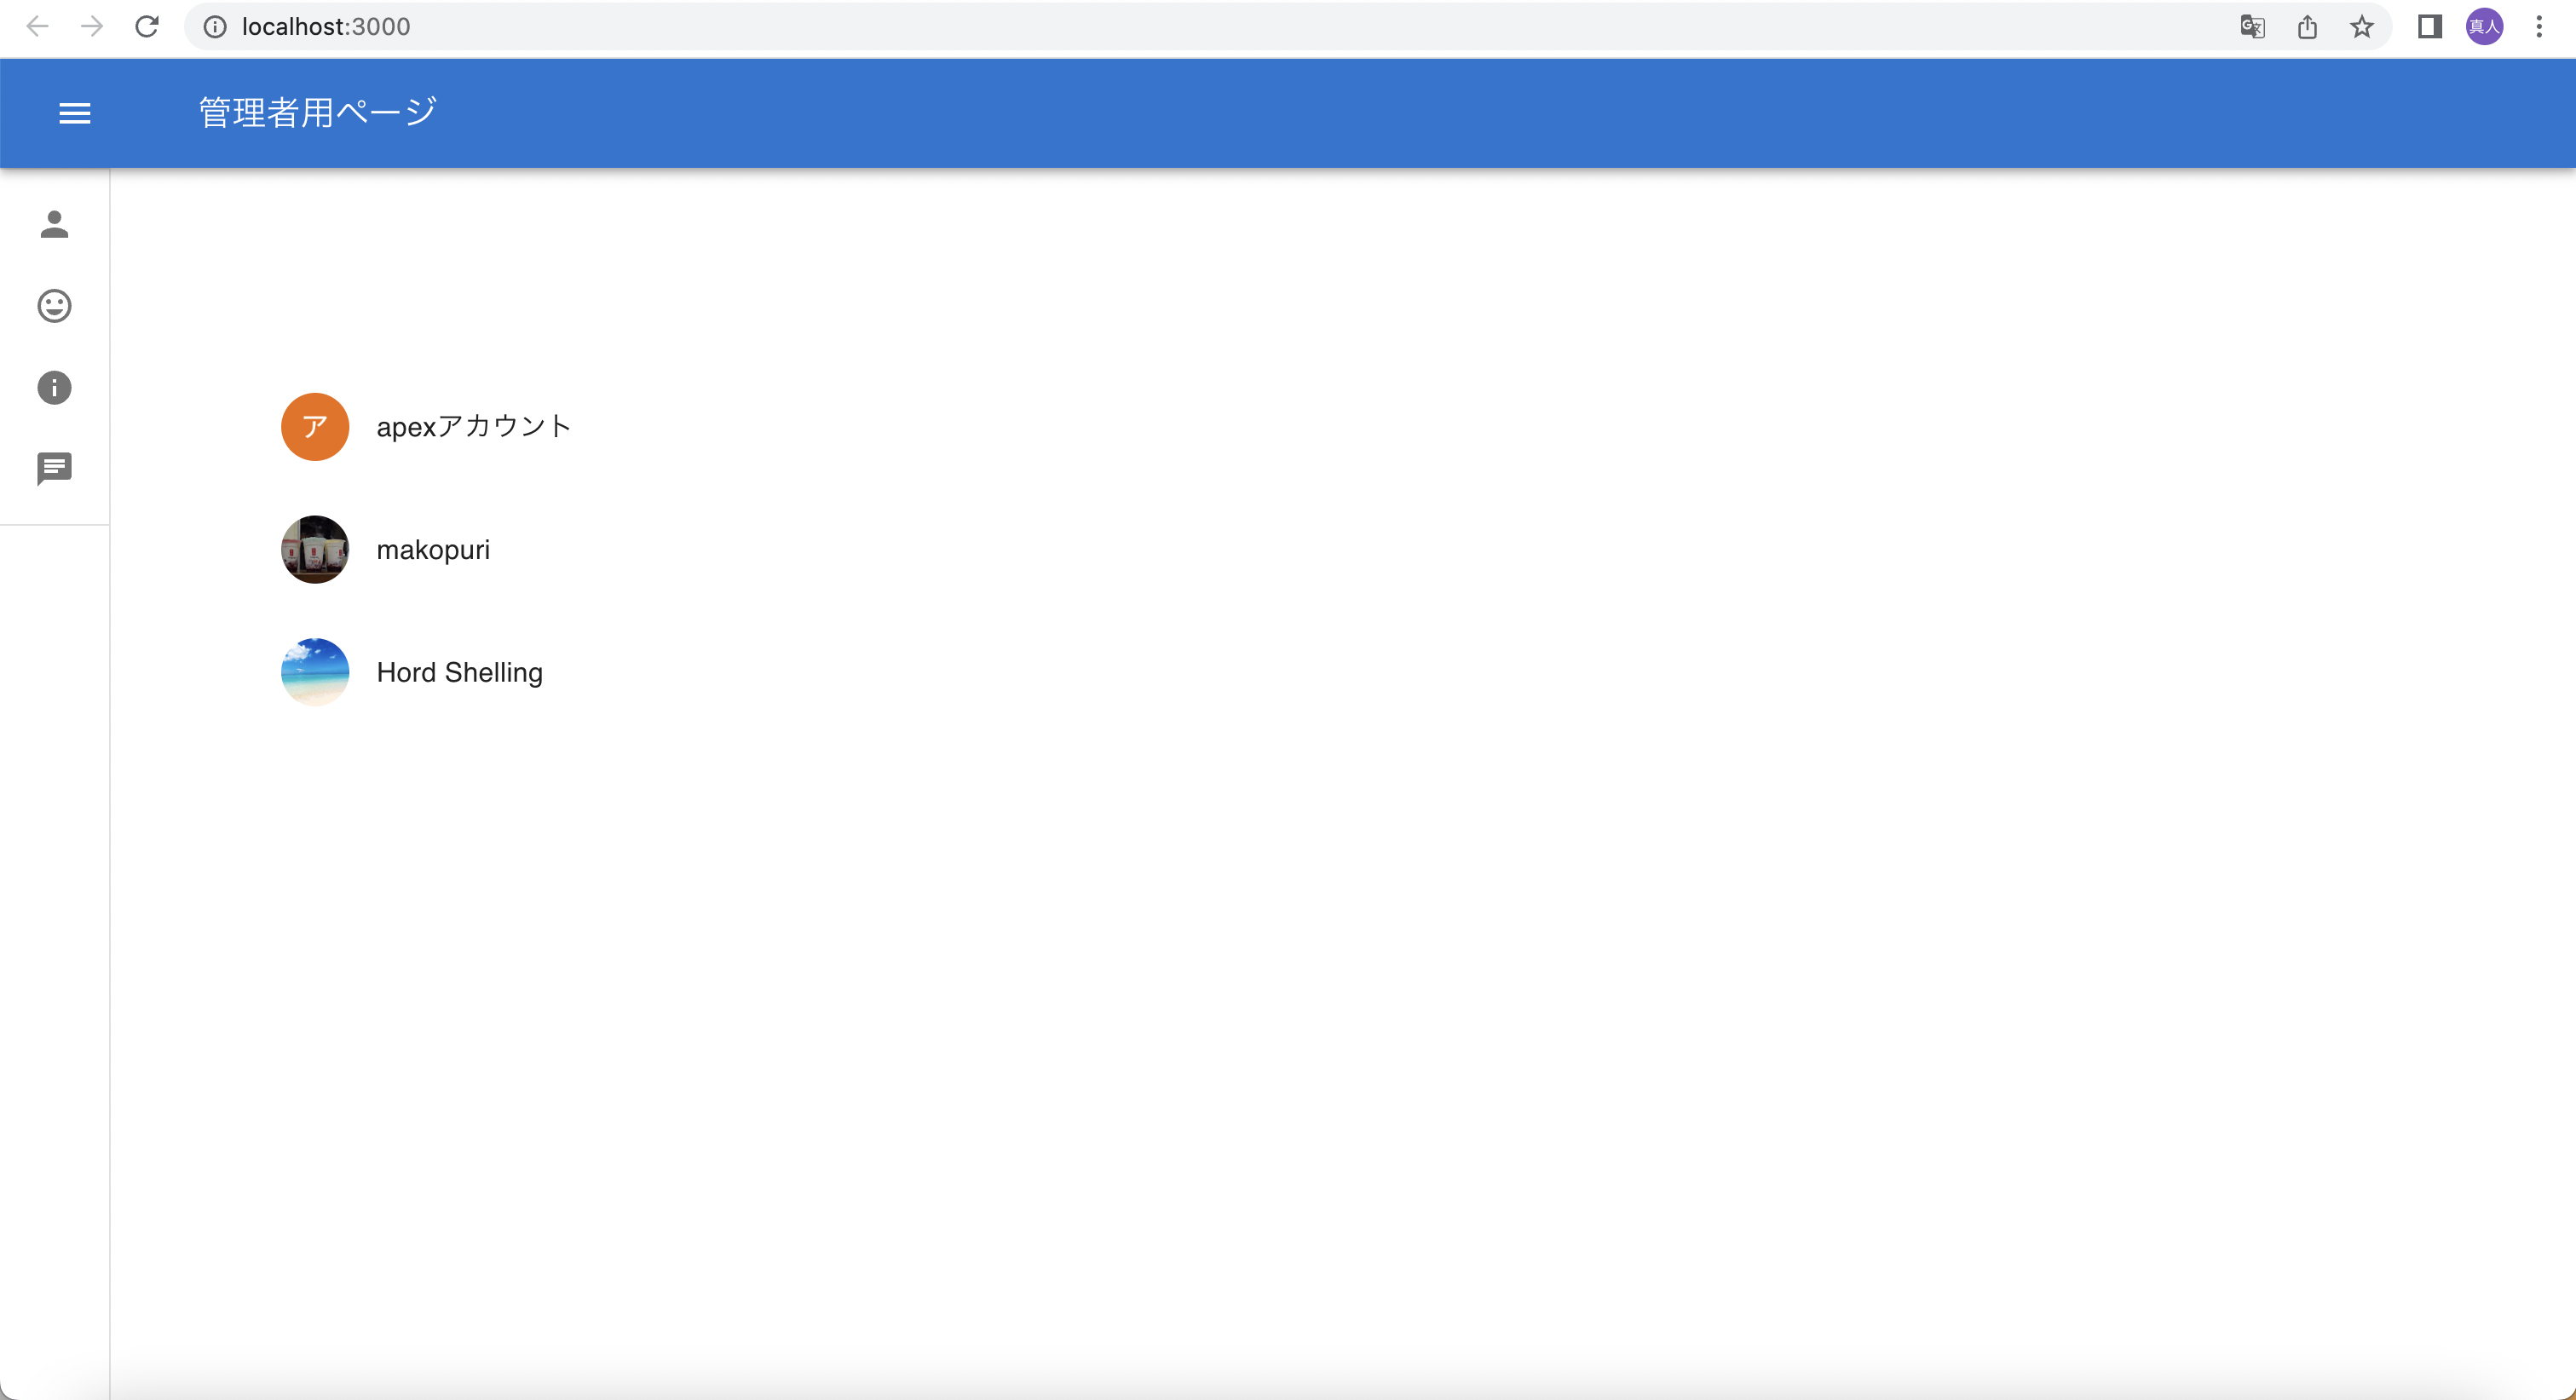
\includegraphics[scale=0.3, clip]{./img/chat5.png}
            \caption{トークリスト画面}
            \label{fig:図の名前}
          \end{center}
          \end{figure}

          \begin{figure}[!h]
            \begin{center}
              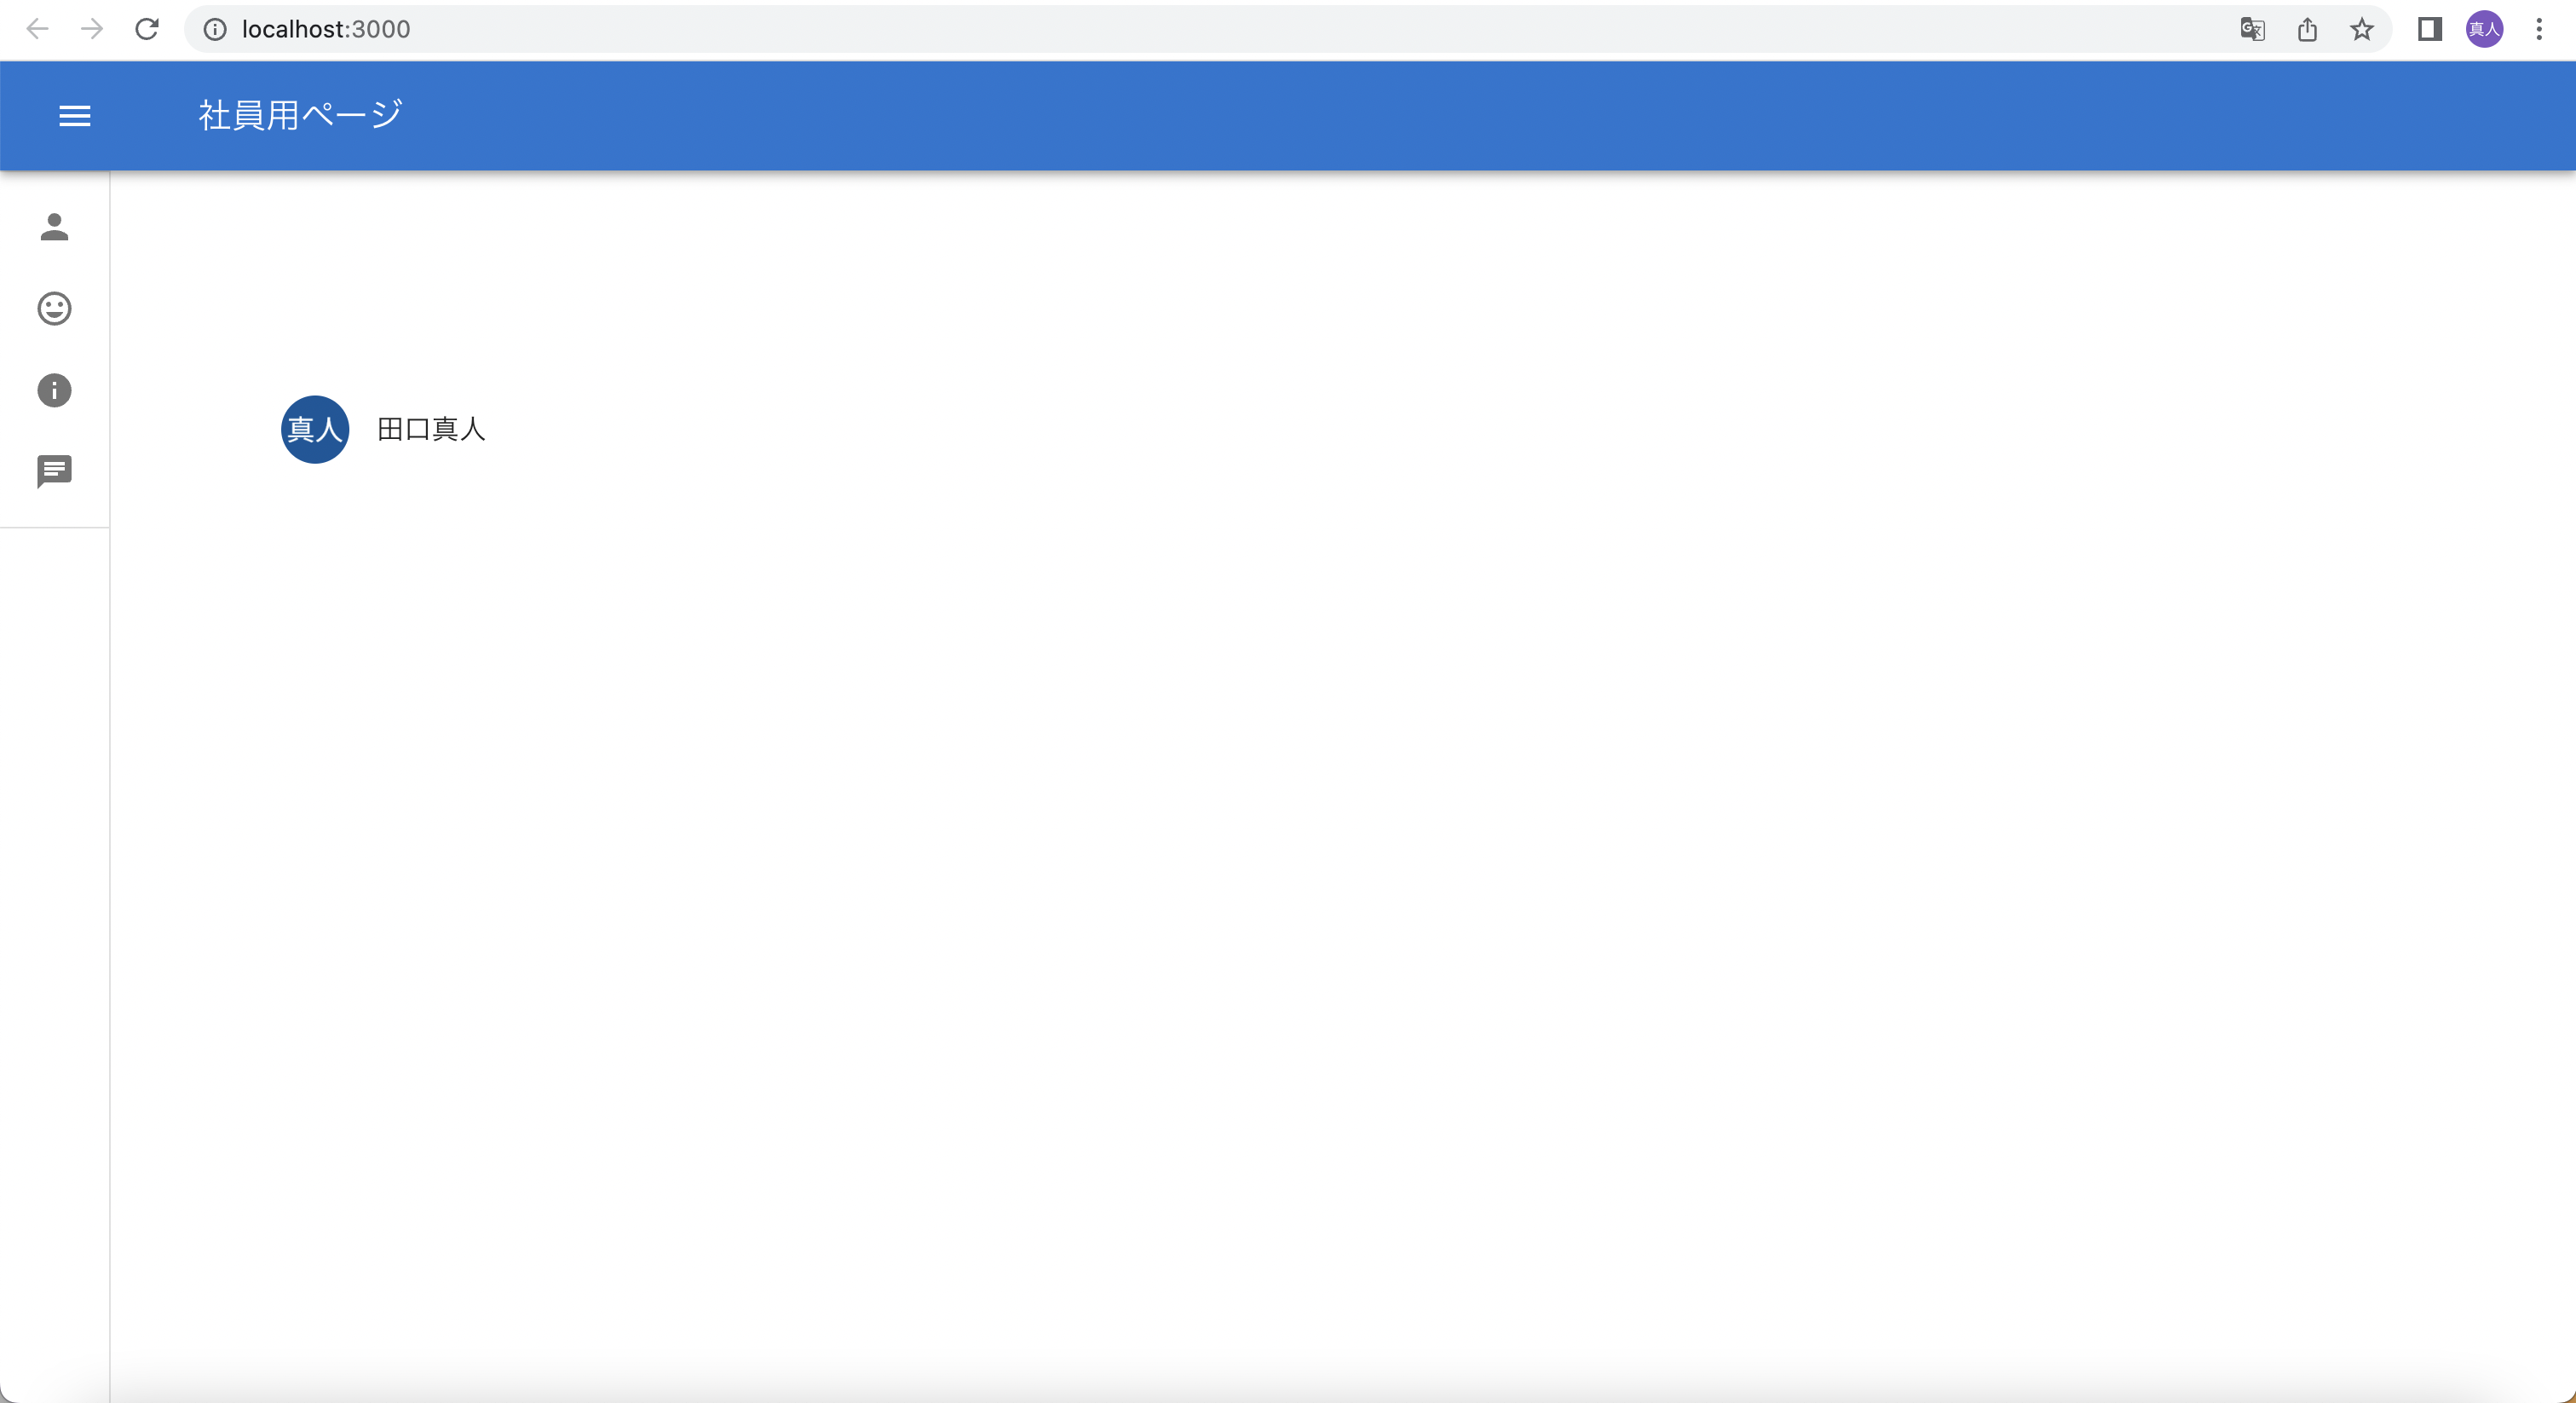
\includegraphics[scale=0.3, clip]{./img/chat6.png}
              \caption{社員用ページのトークリスト画面}
              \label{fig:図の名前}
            \end{center}
            \end{figure}

            \begin{figure}[!h]
              \begin{center}
                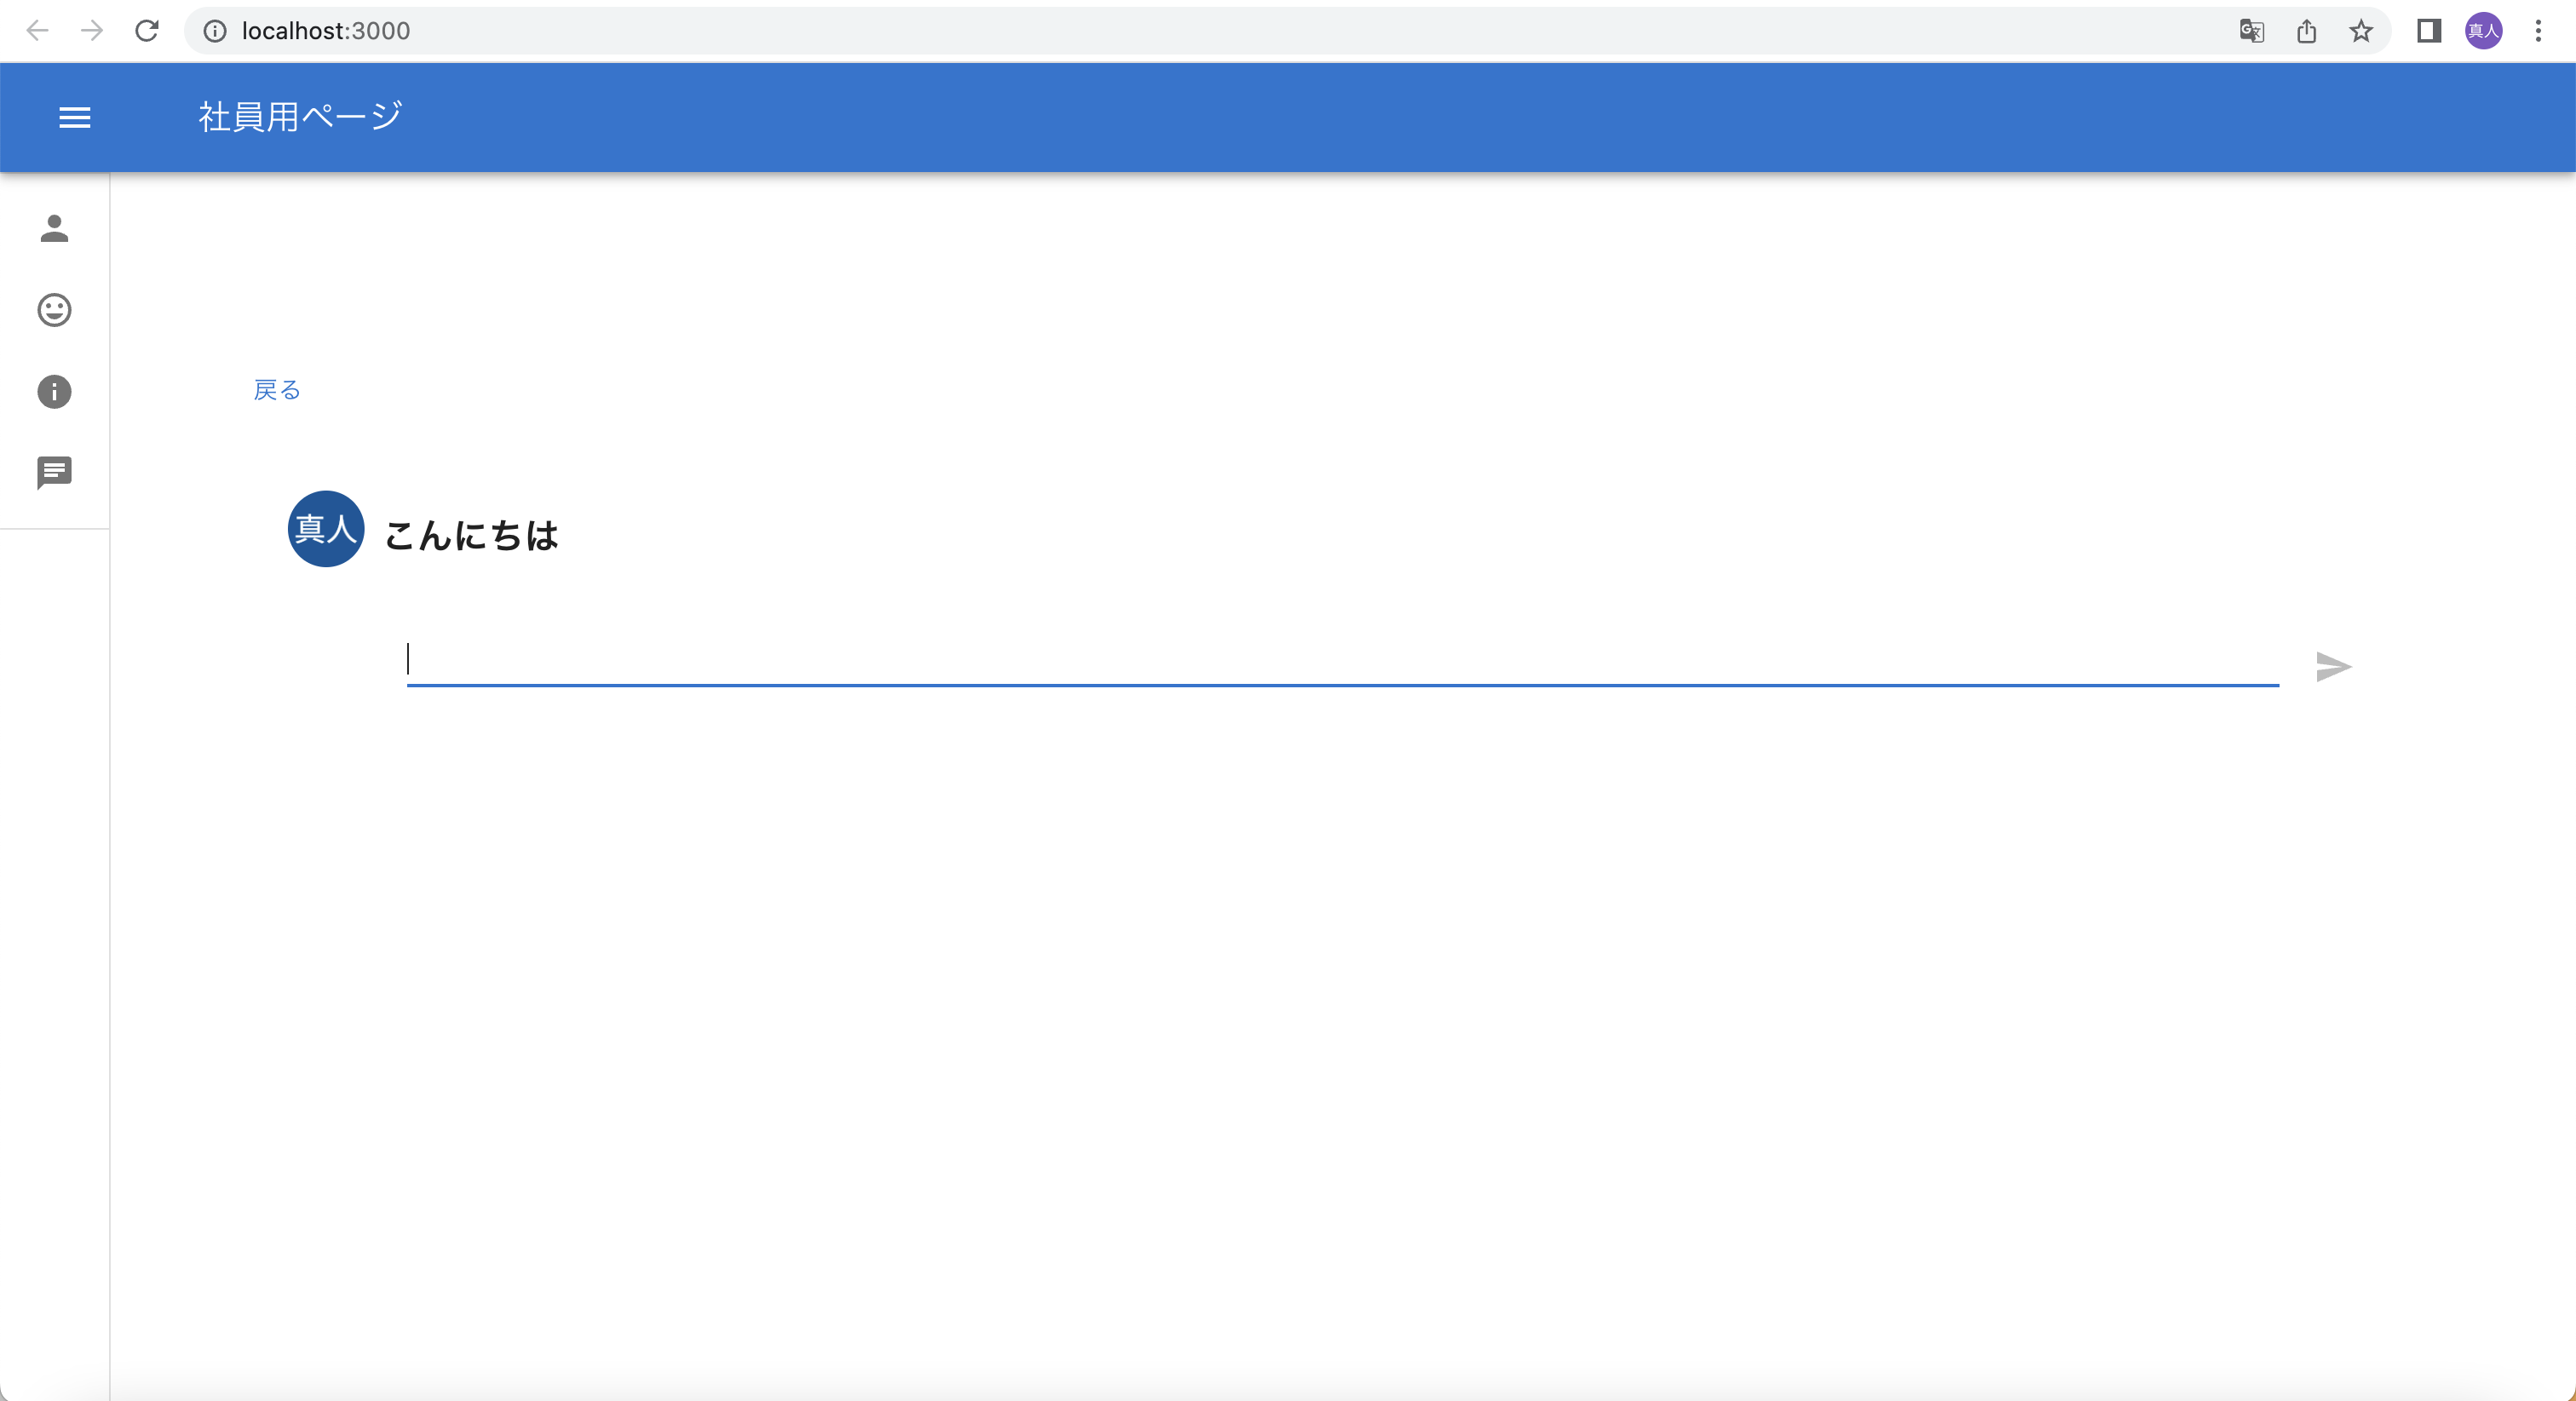
\includegraphics[scale=0.3, clip]{./img/chat7.png}
                \caption{管理者とのトーク画面}
                \label{fig:図の名前}
              \end{center}
              \end{figure}

              \begin{figure}[!h]
                \begin{center}
                  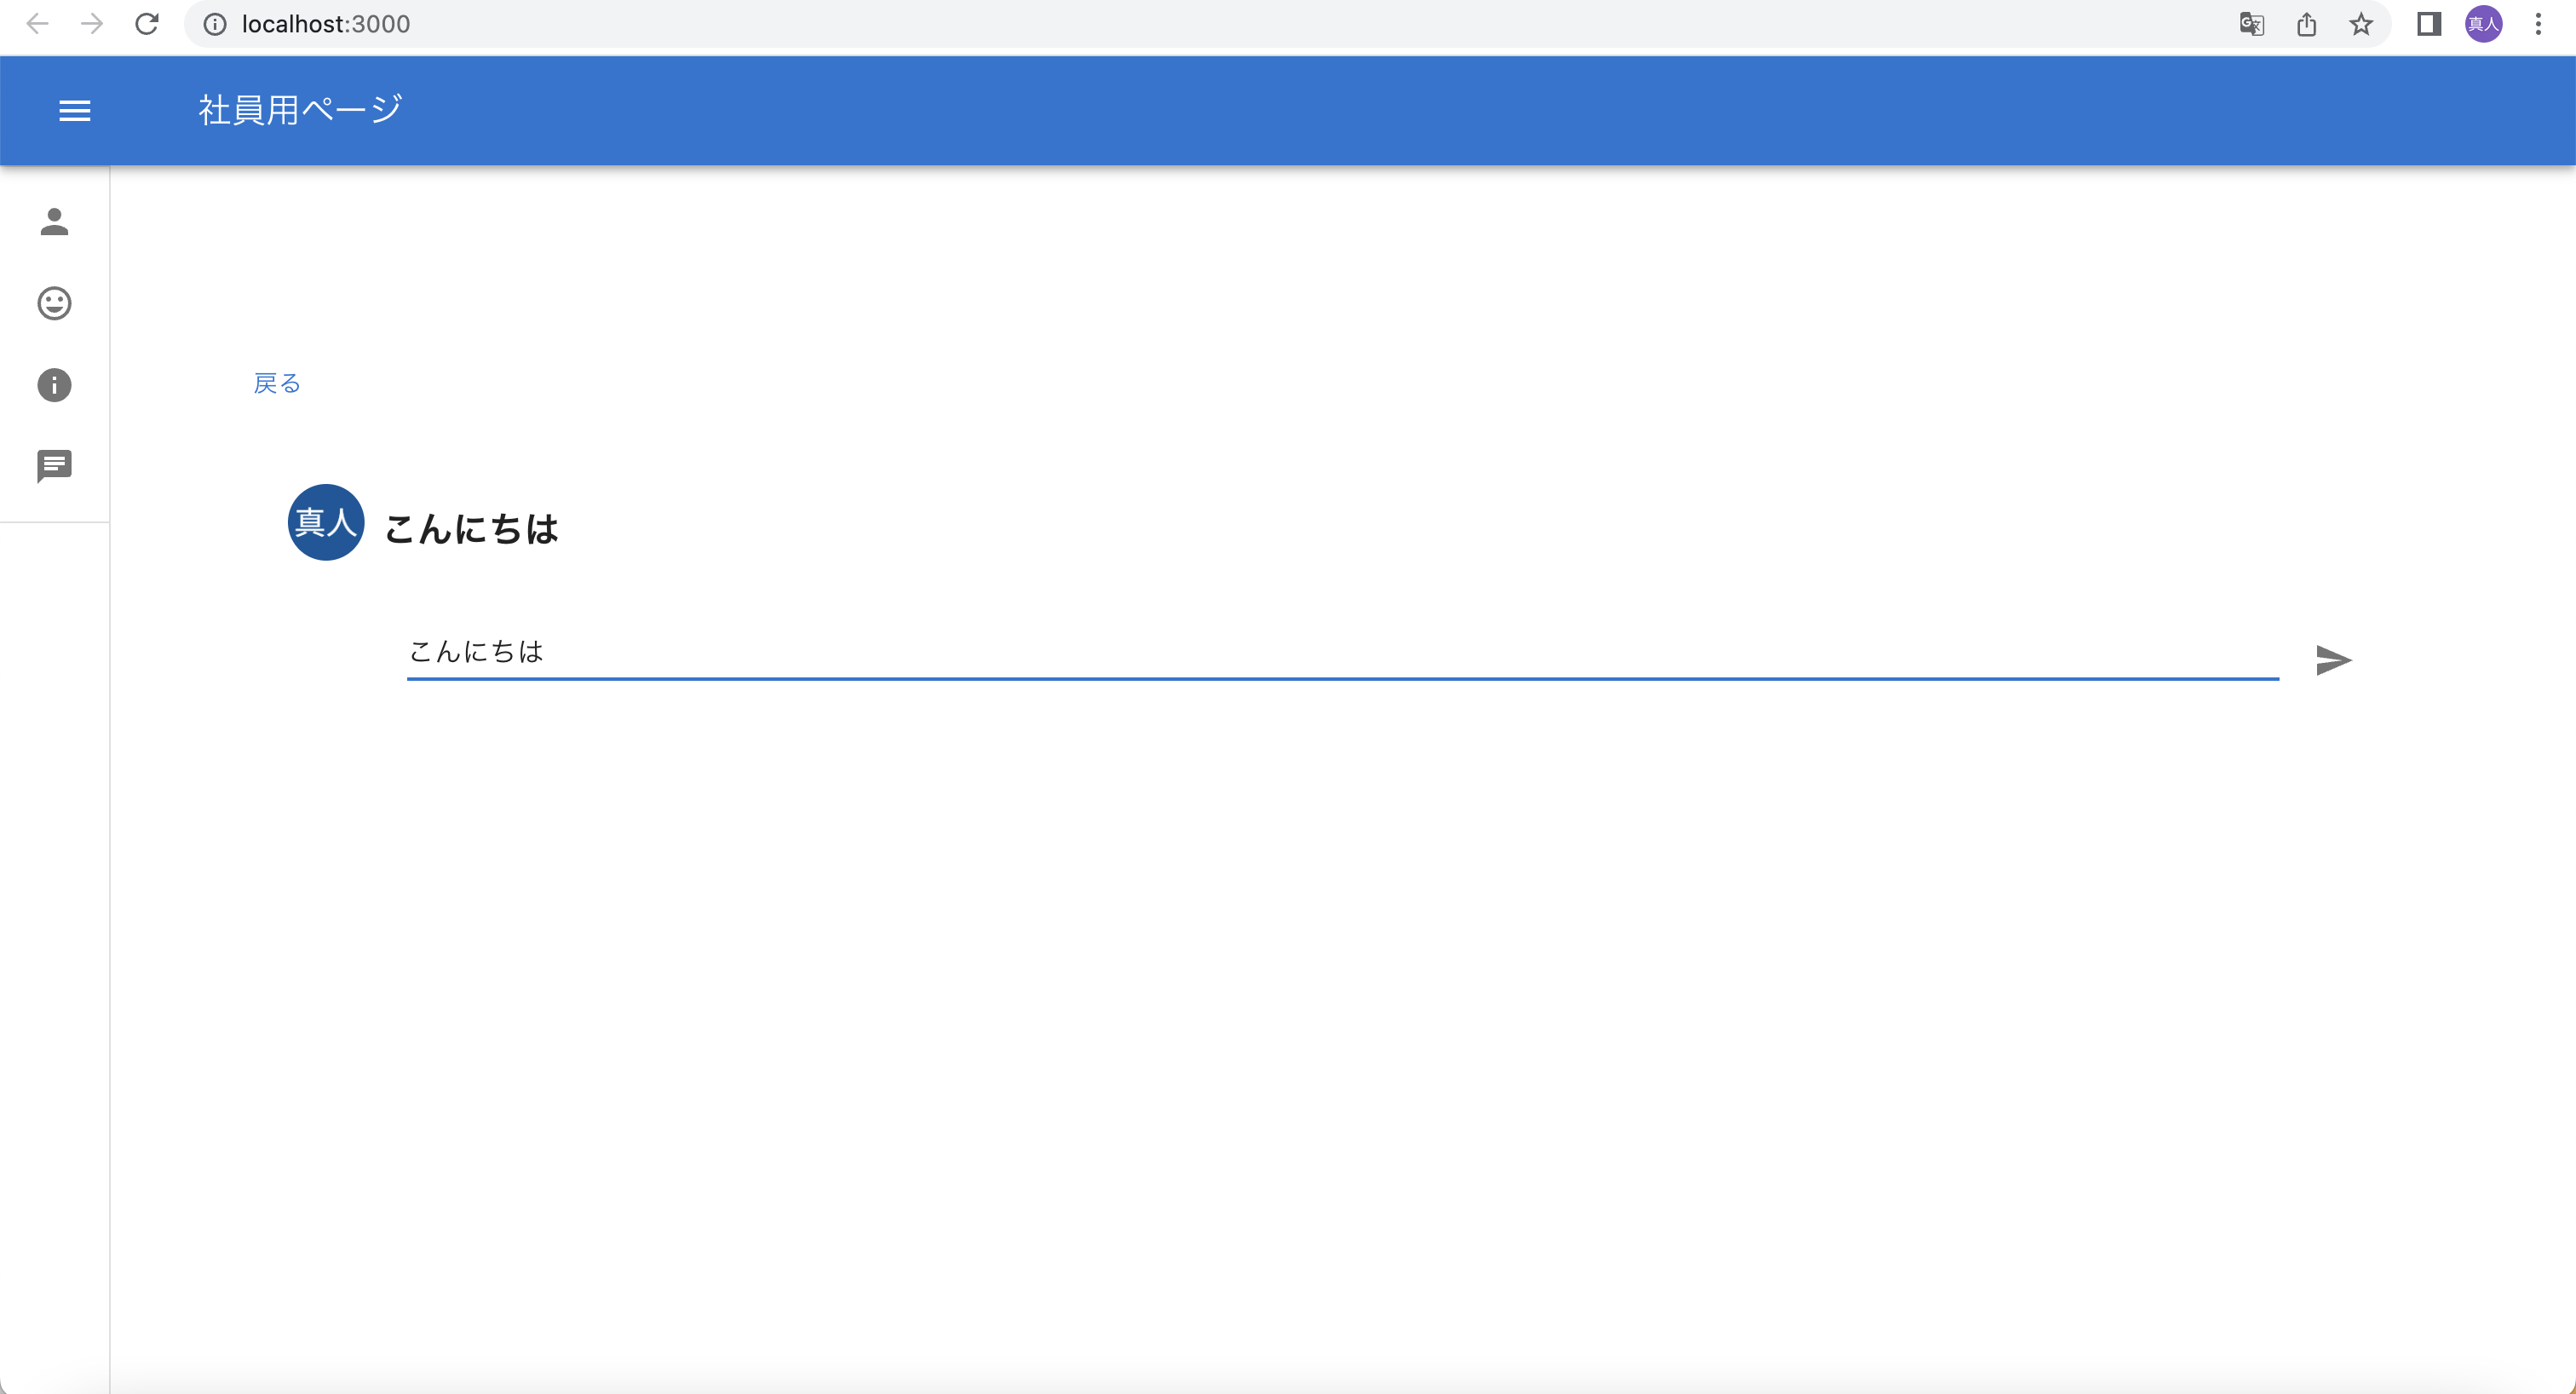
\includegraphics[scale=0.3, clip]{./img/chat8.png}
                  \caption{メッセージ入力画面}
                  \label{fig:図の名前}
                \end{center}
                \end{figure}

                \begin{figure}[!h]
                  \begin{center}
                    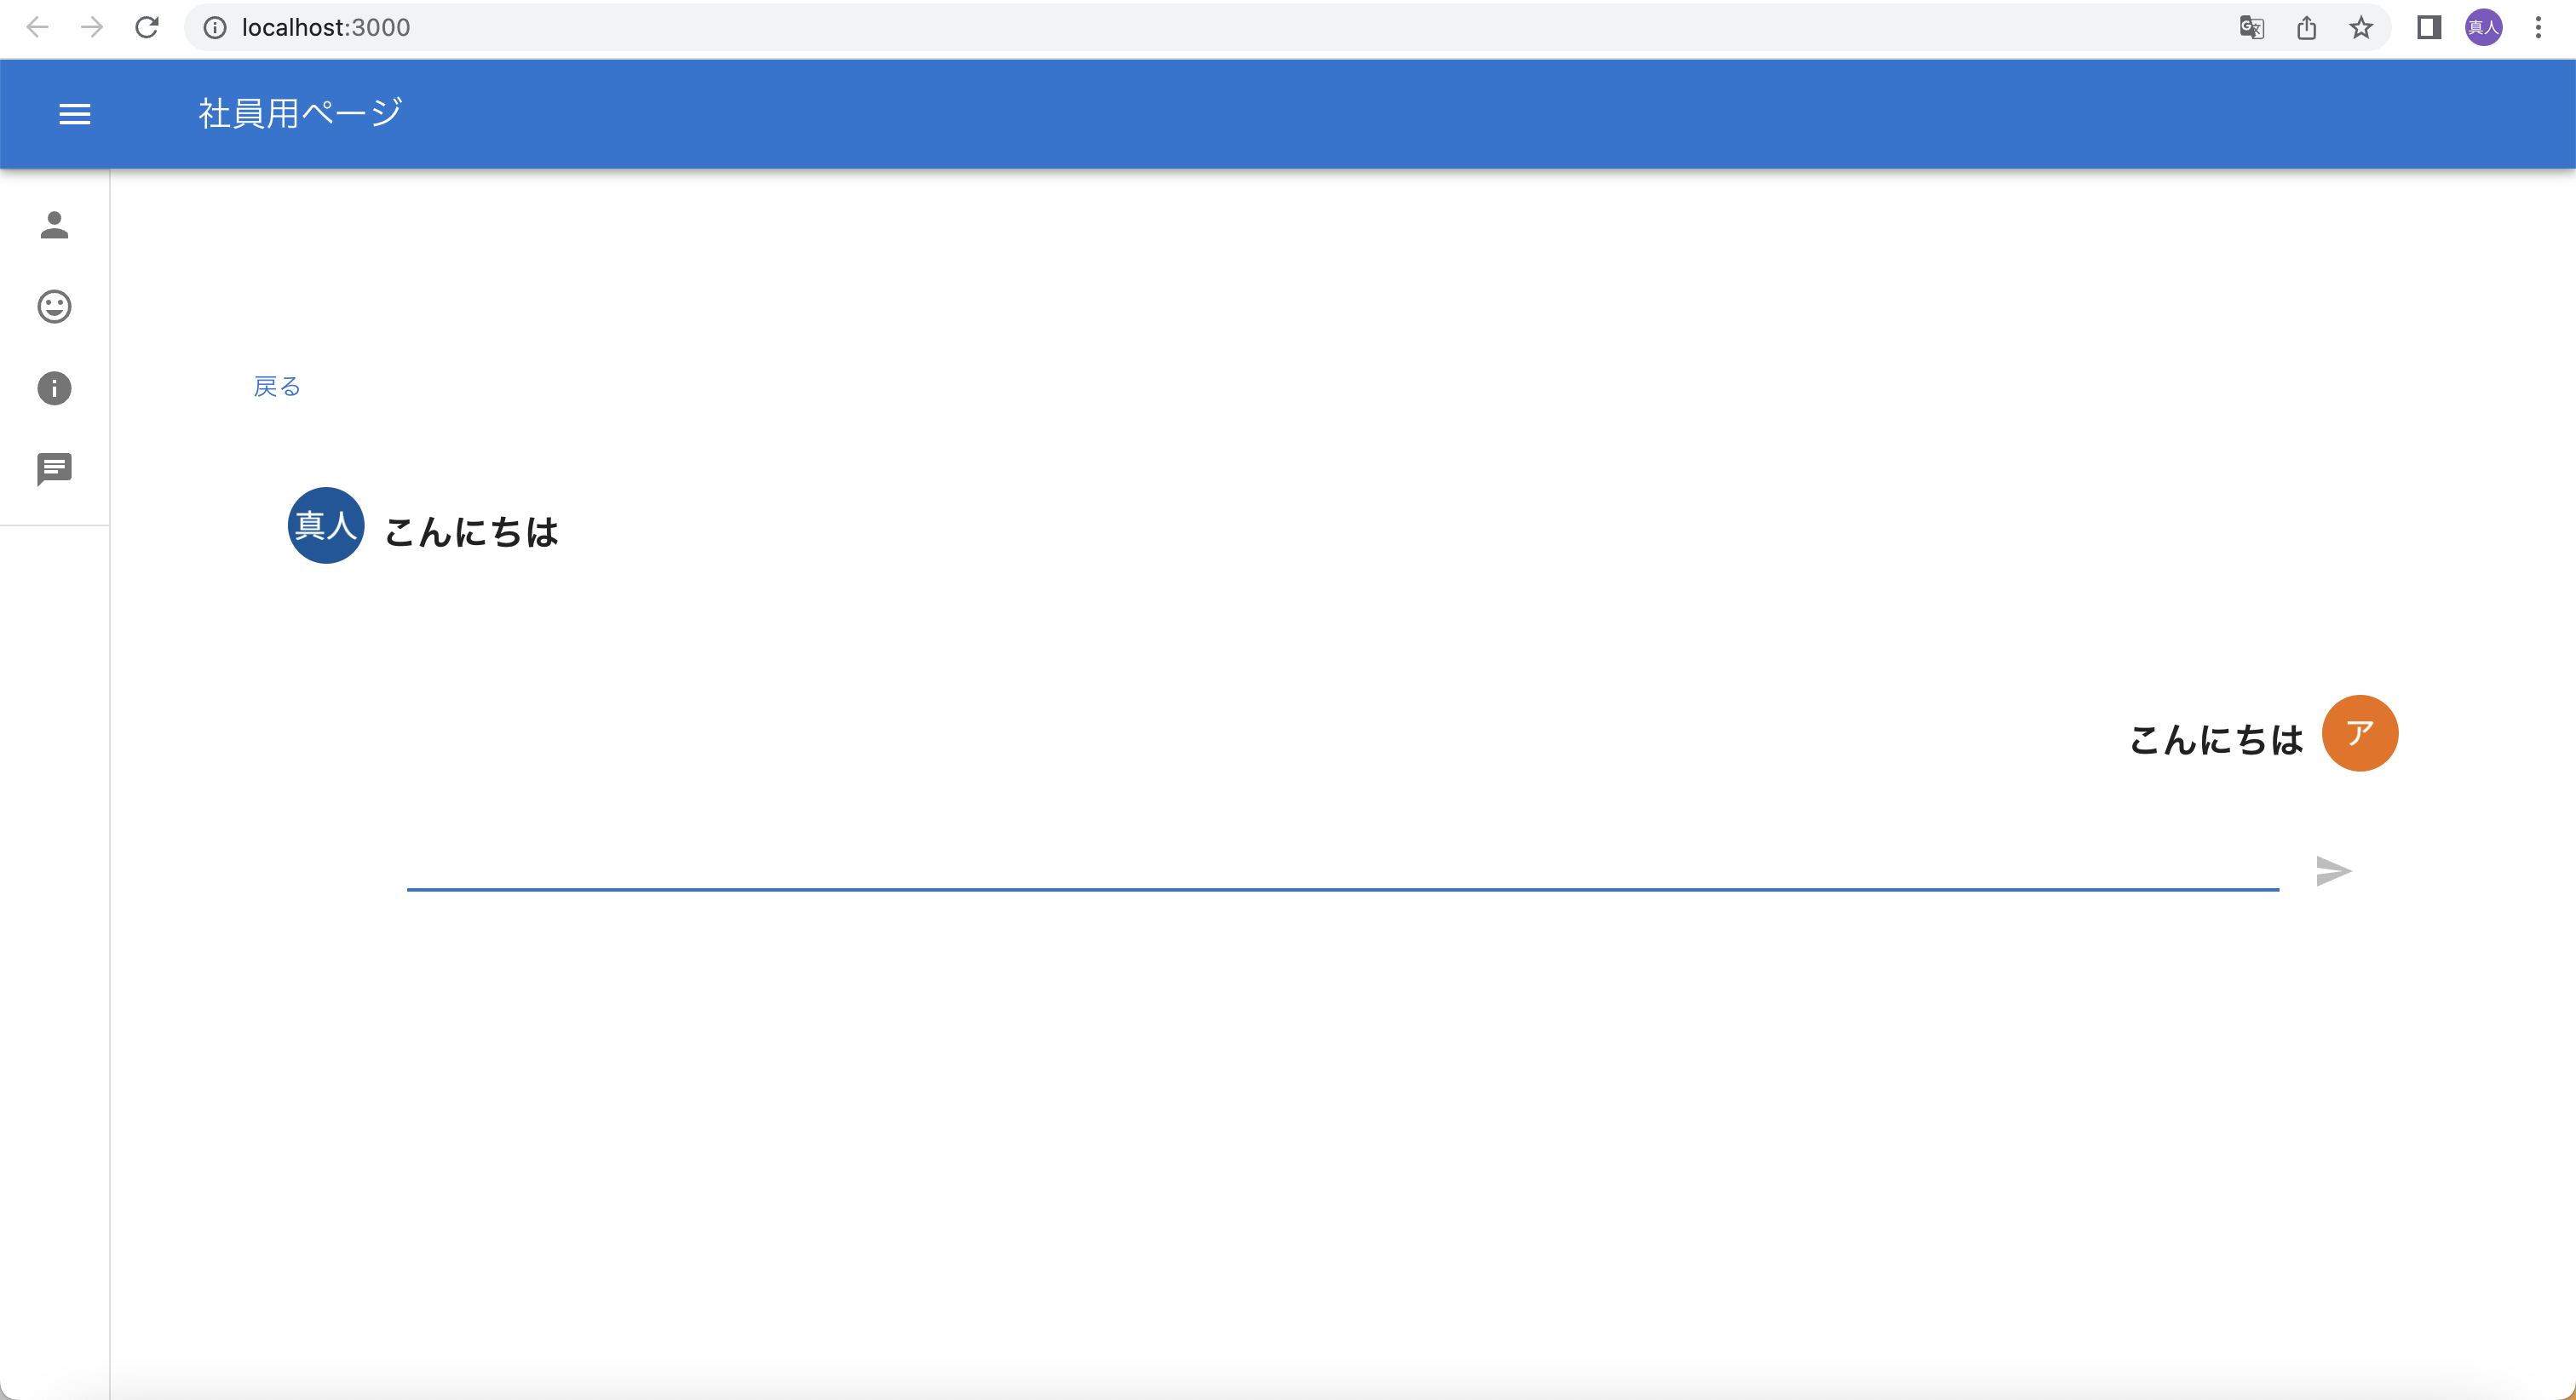
\includegraphics[scale=0.3, clip]{./img/chat9.png}
                    \caption{メッセージ送信した後の画面}
                    \label{fig:図の名前}
                  \end{center}
                  \end{figure}

                  \begin{figure}[!h]
                    \begin{center}
                      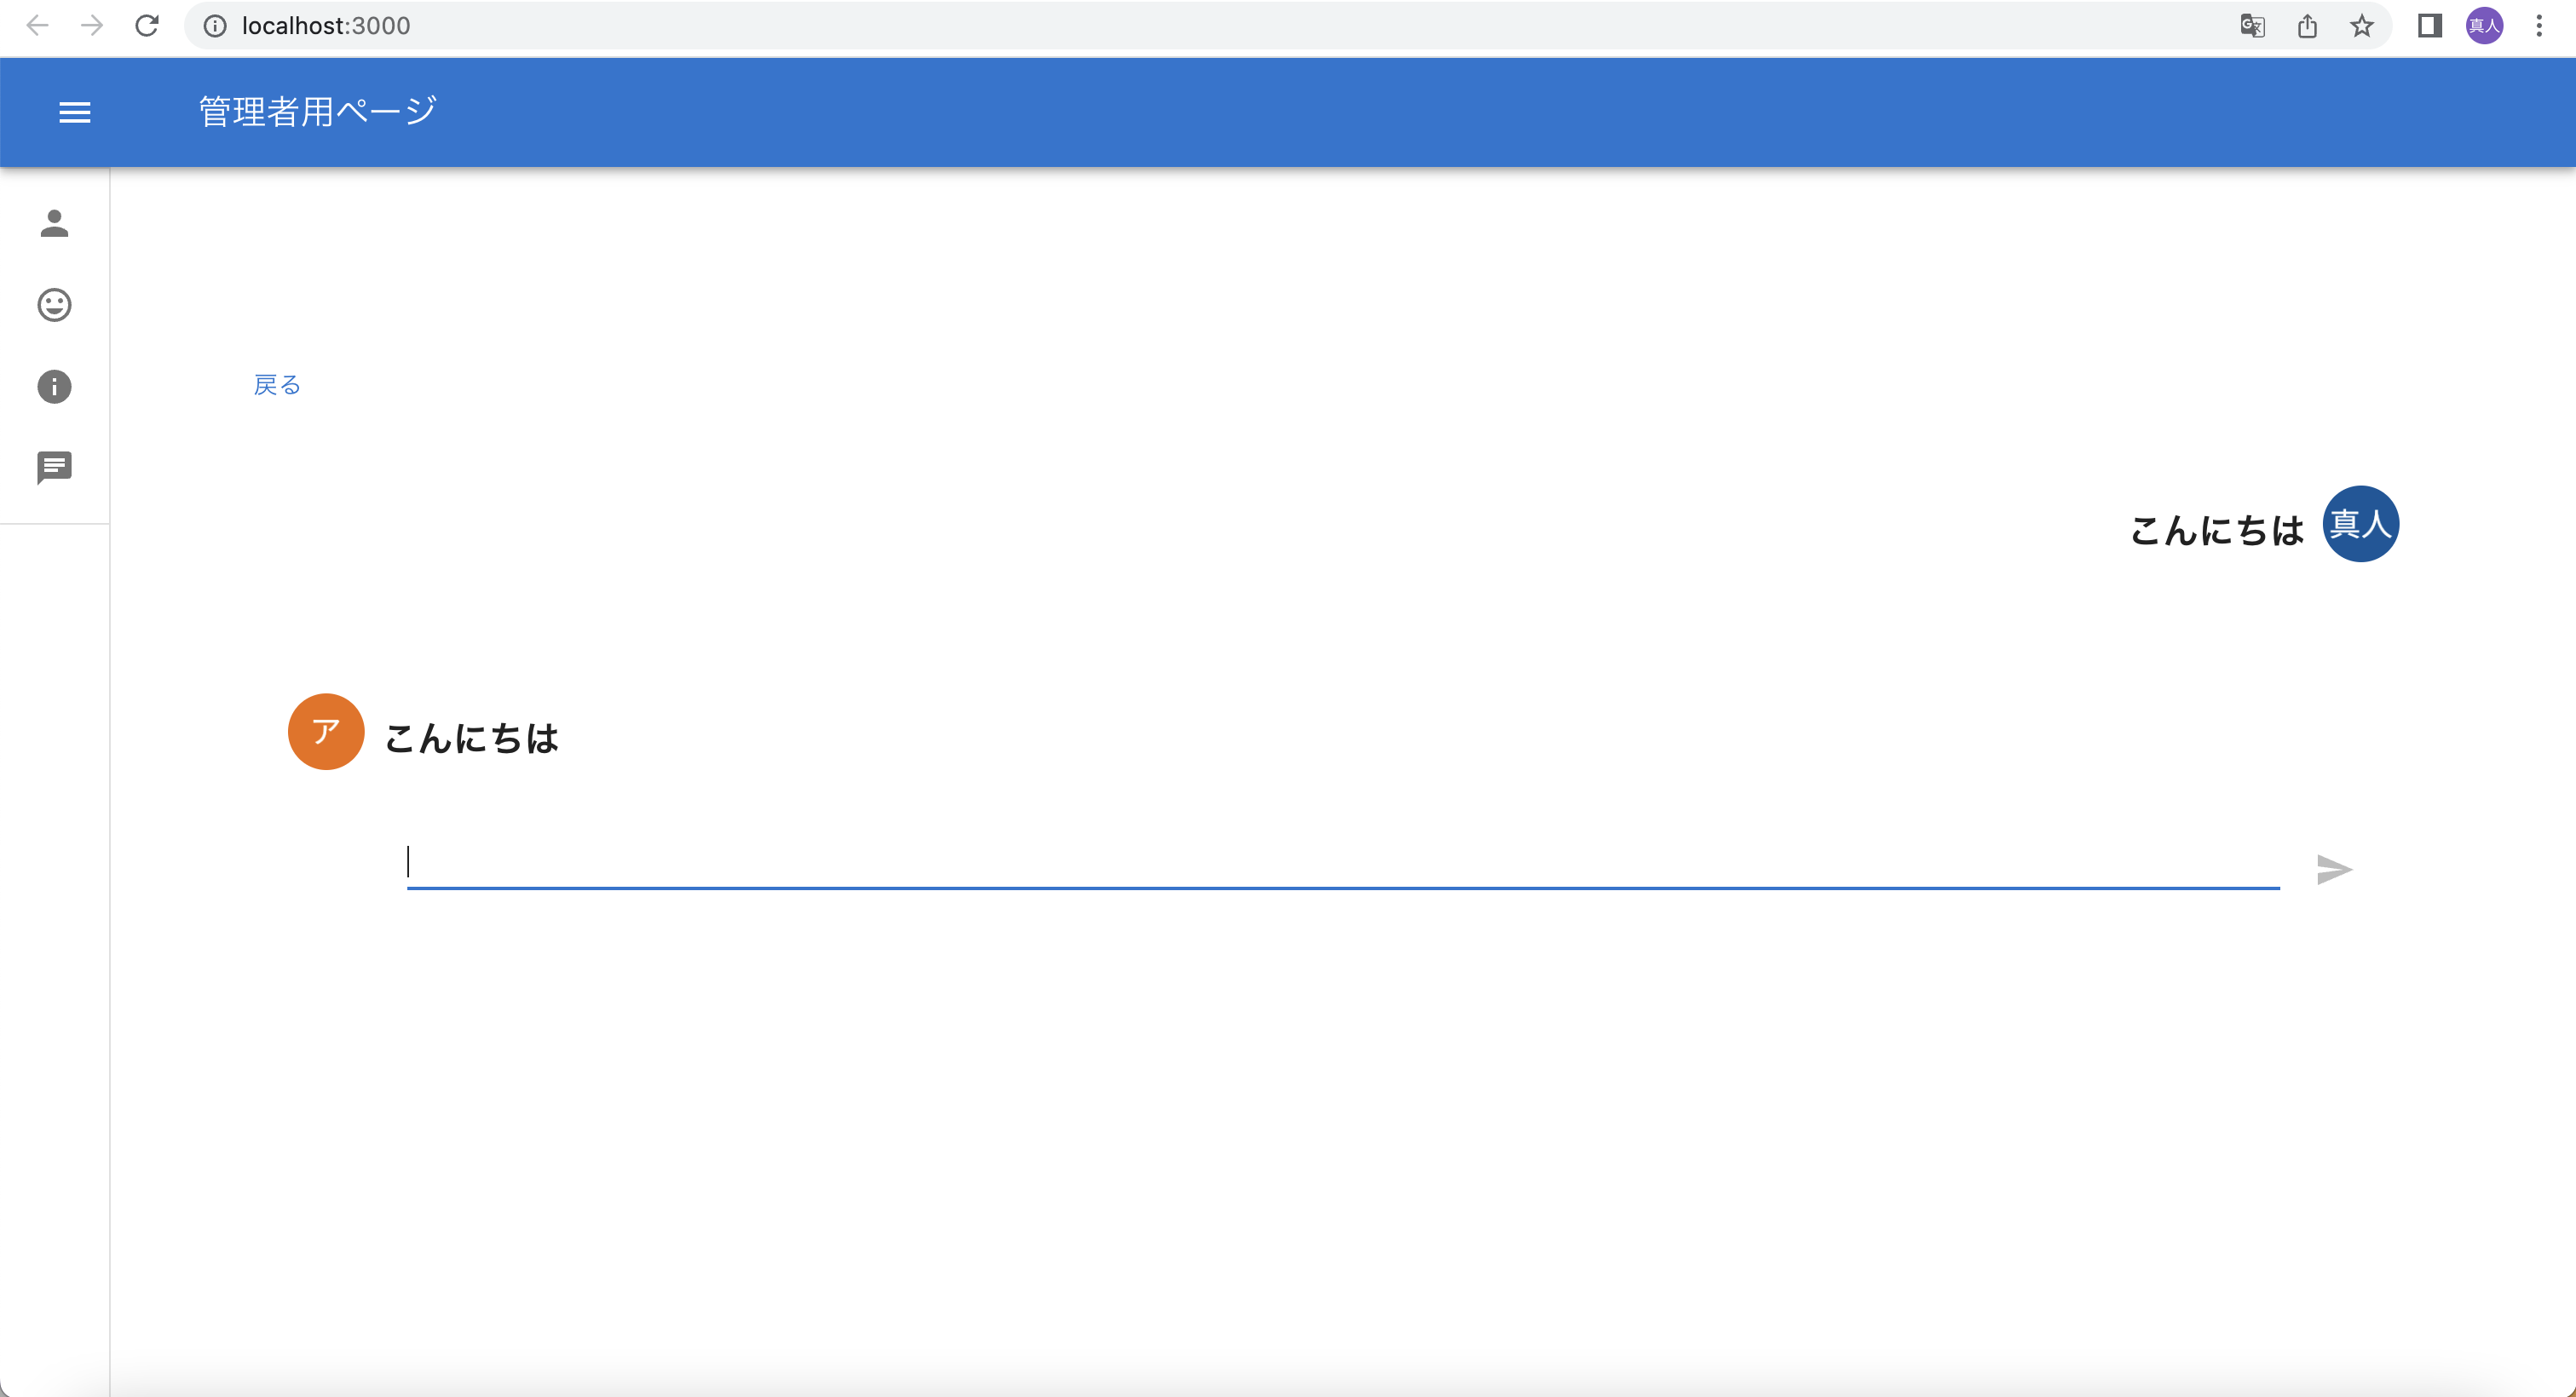
\includegraphics[scale=0.3, clip]{./img/chat10.png}
                      \caption{管理者から見た社員とのトーク画面}
                      \label{fig:図の名前}
                    \end{center}
                    \end{figure}

\newpage

%%%%%%%本文 end%%%%%%%%%%%%%%%%%%%%%%%%%%%%%%%%%%%%%%%%%%%%

%%%%%%%謝辞 start%%%%%%%%%%%%%%%%%%%%%%%%%%%%%%%%%%%%%%%%%%%

\chapter*{ \\謝辞}\addcontentsline{toc}{chapter}{謝辞}
|記述例|

本研究に関しまして,熱心かつ丁寧にご指導いただきました,
千葉工業大学情報科学研究科情報科学専攻中村直人教授に心から御礼申し上げます.
また,修士論文発表における,副査を務めていただきました浮貝雅裕教授,須田宇宙准教授に深謝いたします.
そして,中村研究室博士前期課程,学部生の皆様,および,卒業された博士前期課程,学部生の皆様に心から御礼申し上げます.
皆様のおかげで,これまでの研究生活を充実かつ楽しく送ることが出来ました.
そして,これまで支えてくれた両親をはじめとする親族各位に改めて御礼申し上げます.
ありがとうございました.

%%%%%%%謝辞 end%%%%%%%%%%%%%%%%%%%%%%%%%%%%%%%%%%%%%%%%%%%%

%%%%%%%参考文献 start%%%%%%%%%%%%%%%%%%%%%%%%%%%%%%%%%%%%%%%%%%%
\begin{thebibliography}{99}\addcontentsline{toc}{chapter}{参考文献}

\bibitem{Webデザイン}
Webデザイン編集委員会,“Webデザイン-コンセプトメイキングから運用まで- 改訂版”,CG-ARTS協会(2013).

\bibitem{数値計算法}
三井田惇郎/須田宇宙,“数値計算法 第2版”,森北出版株式会社(2013).


\end{thebibliography}
%%%%%%%参考文献 end%%%%%%%%%%%%%%%%%%%%%%%%%%%%%%%%%%%%%%%%%%%
\end{document}

%%%%%%%コンテンツ end%%%%%%%%%%%%%%%%%%%%%%%%%%%%%%%%%%%%%%%%%%%%